\documentclass{article}

\usepackage{xeCJK}
\usepackage{amsfonts,amssymb}
\usepackage{amsmath}
\usepackage{geometry}
\usepackage{color}
\usepackage{graphicx}

\usepackage{hyperref} 

\usepackage{listings} 
\usepackage{xcolor}
\lstset{
  language=Matlab,  %代码语言使用的是matlab
  frame=shadowbox, %把代码用带有阴影的框圈起来
  rulesepcolor=\color{red!20!green!20!blue!20},%代码块边框为淡青色
  keywordstyle=\color{blue!90}\bfseries, %代码关键字的颜色为蓝色,粗体
  commentstyle=\color{red!10!green!70}\textit,    % 设置代码注释的颜色
  showstringspaces=false,%不显示代码字符串中间的空格标记
  numbers=left, % 显示行号
  numberstyle=\tiny,    % 行号字体
  stringstyle=\ttfamily, % 代码字符串的特殊格式
  breaklines=true, %对过长的代码自动换行
  extendedchars=false,  %解决代码跨页时,章节标题,页眉等汉字不显示的问题
%   escapebegin=\begin{CJK*},escapeend=\end{CJK*},      % 代码中出现中文必须加上,否则报错
  texcl=true}

\geometry{a4paper,scale=0.8}
\geometry{a4paper,left=3.18cm,right=3.18cm,top=2.54cm,bottom=2.54cm}
\linespread{1.5}
\setlength{\parskip}{0.5\baselineskip} % 段落间距

\definecolor{userColor}{RGB}{225,144,52}

\title{Consensus Problems in Networks of Agents\\ with Switching Topology and Time-Delays}
\author{ Jichao Zhao\thanks{E-mail: zhaojichao@imakerlab.cn}}
\date{30-10-2020}

% 正文开始
\begin{document}
\maketitle

% \clearpage
\begin{abstract}
{\color[gray]{0.5}
In this paper, we discuss consensus problems for a network of dynamic agents with fixed and switching topologies. 
We analyze three cases: i) networks with switching topology and no time-delays, ii) networks with fixed topology and communication time-delays, and iii) max-consensus problems (or leader determination) for groups of discrete-time agents. 
In each case, we introduce a linear/nonlinear consensus protocol and provide convergence analysis for the proposed distributed algorithm. 
Moreover, we establish a connection between the Fiedler eigenvalue of the information flow in a network (i.e. algebraic connectivity of the network) and the negotiation speed (or performance) of the corresponding agreement protocol. 
It turns out that balanced digraphs play an important role in addressing average-consensus problems. 
We introduce disagreement functions that play the role of Lyapunov functions in convergence analysis of consensus protocols. 
A distinctive feature of this work is to address consensus problems for networks with directed information flow. 
We provide analytical tools that rely on algebraic graph theory, matrix theory, and control theory. 
Simulations are provided that demonstrate the effectiveness of our theoretical results.
}

这篇文章,我们讨论了动态智能体网络在固定和切换拓扑下的一致性问题。
我们分析了三种情况:i)切换拓扑无时滞网络,ii)固定拓扑有时滞网络,iii)智能体群离散时间下的的最大一致性问题(或领导力问题)。
在每一种情况,我们都介绍了线性/非线性的一致性协议,并且提供了分布式建议算法的收敛性分析。
此外,我们还建立了网络信息流的费德勒特征值(Fiedler eigenvaue)(即网络的代数连通度)和响应一致协议的收敛速度(或性能)之间的联系。
这表明平衡图在解决一致性问题上扮演着重要角色。
我们介绍了在一致性协议的收敛性分析问题中扮演着李雅普诺夫(Lyapunov functions)函数的非一致函数。
这项研究的显著特征是解决了有向信息流网络的一致性问题。
我们提供的分析工具基于代数图论,矩阵论和控制论。
仿真部分提供了我们的理论结果的演示效率。
\end{abstract}

\clearpage
% 生成目录
\tableofcontents

\clearpage
% ------------------------------------------------------------------------------
\section{Introduction}
{\color[gray]{0.5}
Distributed decision-making for coordination of networks of dynamic agents has attracted several researchers in recent years. 
This is partly due to broad applications of multi-agent systems in many areas including cooperative control of unmanned air vehicles (UAVs), flocking of birds [22, 24, 23], schooling for underwater vehicles, distributed sensory networks, attitude alignment of clusters of satellites, and congestion control in communication networks [21].
}

\noindent 这些年,动态智能体网络的分布式决策协调问题吸引了大量的研究者。
部分原因是因为多智能体系统(MAS)在许多领域都有广阔的应用,包括无人协同装置,类鸟集群[22,24,23],水下装置,分布式传感器网络,卫星簇的姿态排列,通信网络的拥挤堵塞控制[21]。

{\color[gray]{0.5}
Agreement problems have a long history in the field of computer science, particularly in automata theory and distributed computation [15]. 
In many applications involving multiagent/multi-vehicle systems, groups of agents need to agree upon certain quantities of interest. 
Such quantities might or might not be related to the motion of the individual agents. 
As a result, it is important to address agreement problems in their general form for networks of dynamic agents with directed information flow under link failure and creation (i.e. variable network topology).
}

一致问题在计算机科学领域具有很长的历史,尤其是在自动控制理论和分布式计算方面[15]。
在很多包含多智能体/复合装置系统和智能体群组的应用需要就大量的利益达成一致。
这些利益也许与单个智能体的运动(不)相关。
至于结果,关于连接失败和新建连接下的定向信息流(即动态网络拓扑),解决动态智能体网络通用形式的一致性问题是非常重要的。

{\color[gray]{0.5}
Our main contribution in this paper is to define and address consensus problems under a variety of assumptions on the network topology (being fixed or variable), presence or lack of communication time-delays, and boundedness of the inputs of dynamic agents. 
In each case, we provide convergence analysis and for linear protocols establish direct connections between performance and robustness of a consensus protocol and the properties of graph Laplacian of the information flow in the network.
}

在这篇文章中,我们主要的贡献是定义和解决了基于许多假设的网络拓扑的一致性问题(固定的和变化的),是否存在通信时滞(time-delays),和输入动态智能体的局限性。
在每种情况,我们都提供了收敛性分析,并且针对线性协议建立了性能和关于图的拉氏变化和一致性协议的鲁棒性之间的定向关系。

{\color[gray]{0.5}
In the past, a number of researchers have worked in problems that are essentially different forms of agreement problems with differences regarding the types of agent dynamics, the properties of the graphs, and the names of the tasks of interest. 
In [25, 7, 6], graph Laplacians are used for the task of formation stabilization for groups of agents with linear dynamics. 
Their method for formation stabilization has not yet been extended to systems with nonlinear dynamics that are not feedback linearizable. 
Special cases of this approach are known as leader-follower type architectures and have been widely used by numerous researchers [19, 4, 14]. 
In [18], graph Laplacians are used in the context of dynamic graph theory. 
In [24, 23], flocking and heading angle alignment for multiple particles is analyzed from the point of view of statistical mechanics and a phase transition phenomenon is observed that occurs the information flow in the network becomes connected. 
The work in [13] focuses on attitude alignment for undirected graphs in which the agents have simple dynamics motivated by the model used in [24]. 
It is claimed that the connectivity of the graph on average is sufficient for convergence of the heading angles of the agents. 
In [20], the authors addressed convergence of linear and nonlinear protocols for networks with undirected graphs in presence or lack of communication time-delays. 
Theoretically, analyzing consensus on directed graphs is more challenging and is considered in the present paper.
}

在过去,大量研究者致力于解决本质上是不同形式的一致性问题,这是智能体是不同类型智能体(异构智能体),图拉普拉斯矩阵的性质,感兴趣任务的命名问题。
在文献[25,7,6]中,图拉普拉斯矩阵被用来解决线性智能体模型的信息稳定问题。
他们的方法没有扩展到非线性智能体系统上,不能反馈线性化。
这种方法的一种熟知的特殊情况是领导者-跟随类型,并且已经被广泛应用在大量的研究中[19,4,14]。
在文献[18],图拉普拉斯矩阵被在动态图论中。
文献[24,23]中,多重粒子的群集问题和航向角问题从统计力学的角度进行了分析,并且观察到发生在网络中的信息流的相转换现象变的相互连接。
文献[13]的工作集中在无向图的姿态对齐问题,这里的智能体采用的文献[24]中的简单动态模型。
可以断定,图的平均连通性对于智能体的航向角收敛是有效的。
文献[20]解决了有(无)时滞的无向图系统的线性和非线性系统模型一致性问题。
理论上,有向图的一致性分析更具有挑战性,并且在接下来的文献中进行讨论。

{\color[gray]{0.5}
In this paper, we provide convergence analysis of consensus protocol for a network of integrators with a directed information flow and fixed or switching topology. 
Our analysis relies on several tools from algebraic graph theory [1, 11] and matrix theory [12]. 
We establish a connection between the performance of the linear consensus protocol and the Fiedler eigenvalue of graph Laplacian of a graph called the mirror graph (that is closely-related to the original directed graph).
}

本文,我们提供了有向信息流固定和切换拓扑网络的一致性协议收敛分析。
我们的分析依赖于一些代数图论[1,11]和矩阵论[12]的工具。
我们建立了线性一致性协议的性能和镜像图拉普拉斯矩阵的费德勒特征值之间的联系(镜像图与原来的有向图密切相关)。

{\color[gray]{0.5}
It turns out that a class of directed graphs called balanced graphs have a crucial role in derivation of an invariant quantity and a Lyapunov function for convergence analysis of average-consensus problems on directed graphs. 
This Lyapunov function is a measure of group disagreement in the network. 
We show that a directed graph solves the average-consensus problem using a certain protocol if and only if it is balanced. 
Furthermore, we use properties of balanced networks to analyze the convergence of an agreement protocol for networks with switching topology. 
This variation of the network topology is usually due to link failures or creations in networks with mobile nodes. 
We introduce a common Lyapunov function that guarantees asymptotic convergence to a group decision value in a network with switching information flow.
}

结果表明,一类称为平衡图的有向图在求导不变量和李雅普诺夫(Lyapunov)函数对有向图上平均一致问题的收敛性分析中起着至关重要的作用。
这个李亚普诺夫函数是对网络中群组非一致性的衡量。
我们证明了当且仅当图是平衡图时,有向图可以使用一个确定的协议解决平均一致性问题。
进一步,我们使用图的性质分析了切换拓扑网络的一致性收敛协议。
网络拓扑图的变化通常是由于网络中模型节点之间连接的失败或重新建立造成的。
我们介绍了一个常用的李亚普诺夫函数,来保证切换信息流网络能够渐进收敛到群组决策值(decision value)。

{\color[gray]{0.5}
Building on these basic results, we provide a number of extensions. 
We discuss the effects of communication time-delays in solving consensus problems. 
For undirected graphs, we address average-consensus problem under the constraint that the inputs of all agents are bounded. 
This leads to analyzing a nonlinear protocol. 
Using a example of a network with three nodes, we demonstrate that analyzing the convergence of this protocol for general digraphs is a challenging open problem. 
Finally, we pose and address the max-consensus problem that is useful for determining a superior or leader in a group of agents in a distributed way.
}

在这些基本结果的基础上,我们提出了一些扩展。
我们讨论了通信时滞在解决一致性问题中的影响。
对于无向图,我们基于所有智能体的输入都是有界的约束下解决了平均一致性问题。
这引导分析了非线性协议。
使用一个三节点的例子,我们演示了分析该协议对于一般有向图的收敛性是一个具有挑战性的开放问题。
最后,我们提出并解决了最大一致性问题,这对以分布式方式决定智能体群中的先导者(superior)或领导者(leader)是有用的。

{\color[gray]{0.5}
Simulation results are provided that demonstrate our theoretical predictions and show the novel analytical tools that we propose are effective.
}

我们提供了仿真结果,演示了我们的理论预测,并演示了我们提出的新的分析工具的有效性。

{\color[gray]{0.5}
An outline of this paper is as follows. 
In Section 2, we define consensus problems. 
In Section 3, we give two protocols. 
Some background on algebraic graph theory and properties of graph Laplacians are provided in Section 4. 
A counterexample is given in Section 5 that shows not every digraph solves an average-consensus problem. 
In Section 6, our main results on networks with switching topology are presented. 
Average-consensus problems for networks with communication time-delays is discussed in Section 7. 
In Section 8, our result on max-consensus problem is given. 
The simulation results are presented in Section 9. 
Finally, in Section 10, concluding remarks are stated.
}

本文大纲如下。
第2部分,我们定义了一致性问题。
第3部分,我们给出了两个协议。
第4部分,展示了代数图论的一些背景知识和图拉普拉斯矩阵的一些性质。
第5部分,给出了一个反例,表明不是所有的图都能解决平均一致性问题。
第6部分,是我们在切换拓扑方面的主要结果。
第7部分,讨论了网络有通信时滞的平均一致性问题分析。
第8部分,给出了我们对最大一致性问题的结果。
第9部分,展示了仿真结果。
最后,第10部分,展示了结论和总结。

% ------------------------------------------------------------------------------
\section{Consensus Problems}
{\color[gray]{0.5}
Let $G=(\mathcal{V},\mathcal{E},\mathcal{A})$ be a weighted directed graph (or digraph) with $n$ nodes and a weighted adjacency matrix $\mathcal{A}=[a_{ij}]$ where $a_{ij} \ge 0$ for all $i,j \in \mathcal{I}={1,2,…,n}$ with $i \ne j$. 
Here, $\mathcal{V}$ denotes the set of vertices $v_i$ and $\mathcal{E}$ denotes the set of edges $ij$ (or ($v_i,v_j$)) of the graph $G$. 
The set of neighbors of node $i$ is denoted by $N_i=\{ij\in \mathcal{E}:a_{ij}>0\}$. 
We call any subset of nodes $J$ a cluster. 
The set of neighbors of a cluster $J\subset \mathcal{I}$ is defined by
}

\noindent 定义$G=(\mathcal{V},\mathcal{E},\mathcal{A})$具有$n$个节点,和一个加权邻接矩阵$\mathcal{A}=[a_{ij}]$的加权有向图(或普通图),$\mathcal{A}$矩阵的所有元素$a_{ij} \ge 0$且所有的$i,j \in \mathcal{I}={1,2,…,n},i \ne j$。
这里,$\mathcal{V}$表示所有向量$v_i$的集合,$\mathcal{E}$表示图中所有边$ij$(或$v_i,v_j$)的集合。
节点$i$的邻居集合表示为$N_i=\{ij\in \mathcal{E}:a_{ij}>0\}$。
我们称节点$J$的任意子集为一个簇。
簇$J\subset \mathcal{I}$的集合定义为
\begin{equation}
    N_J:=\cup_{i\in J}N_i=\{j\in \mathcal{I}:i\in J, ij\in \mathcal{E}\}
    \tag{1}
    \label{1}
\end{equation}

{\color[gray]{0.5}
Let $x_i\in \mathbb{R}$ denote the value of node $i$. 
We refer to $G_x=(\mathcal{V},\mathcal{E},\mathcal{A},x)$ with $x=(x_1,...,x_n)^T$ as an algebraic graph or (static) network with value $x\in \mathbb{R}^n$ and information flow $G=(\mathcal{V},\mathcal{E},\mathcal{A})$. 
The value of a node might represent physical quantities including attitude, position, temperature, voltage, and so on. 
We say nodes $i$ and $j$ in a network agree if and only $x_i=x_j$. 
We say all the nodes in a network have reached a consensus if and only if $x_i=x_j$ for all $i,j\in \mathcal{I}, i\ne j$. 
Whenever the nodes of a network are in agreement, the common value of all nodes is called the (group) decision value.
}

定义$x_i\in \mathbb{R}$表示节点$i$的值。
我们将具有$x=(x_1,...,x_n)^T$的$G_x=(\mathcal{V},\mathcal{E},\mathcal{A},x)$,称作是一个代数图,或具有$x\in \mathbb{R}^n$的信息流(静态)网络$G=(\mathcal{V},\mathcal{E},\mathcal{A})$。
节点的值表示物理特性,例如姿态,位置,温度,电压等等。
我们认为当且仅当$x_i=x_j$时,节点$i$和$j$在网络中达到一致(agree)。
我们认为网络中所有的节点当且仅当所有的$x_i=x_j$时达到一致(consensus),此时$i,j\in \mathcal{I}, i\ne j$。
当网络中的节点达到一致时,此时所有节点的公共值叫做(群组)决策值。

{\color[gray]{0.5}
Suppose each node of a graph is a dynamic agent with dynamics
}

假设图的每一个节点都是一个具有动态性能的动态智能体

\begin{equation}
    \dot{x}_i = f(x_i, u_i), i\in \mathcal{I}
    \tag{2}
    \label{2}
\end{equation}

{\color[gray]{0.5}
\noindent A dynamic graph (or dynamic network) is defined as a 4-tuple $G_{x(t)} = (\mathcal{V},\mathcal{E},\mathcal{A},x(t))$ together with dynamics $\dot{x}=F(x,u)$ where $x$ denotes the state of the dynamic graph and $F(x,u)$ is the column-wise concatenation of the elements $F_i(x,u)=f(x_i,u_i)$.
}

\noindent 一个动态图或(动态网络)定义为随着$\dot{x}=F(x,u)$动态变化的的4元组$G_{x(t)} = (\mathcal{V},\mathcal{E},\mathcal{A},x(t))$,其中$x$表示动态图的状态,$F(x,u)$是$F_i(x,u)=f(x_i,u_i)$中元素的列合并。

{\color[gray]{0.5}
Let $\chi: \mathbb{R}^n \rightarrow \mathbb{R}$ be a function of $n$ variables $x_1,\dots,x_n$. 
The $\chi$-consensus problem in a dynamic graph is a distributed way to calculate $\chi(x(0))$ by applying inputs $u_i$ that only depend on the values of node $i$ and its neighbors. 
We say a protocol
}

定义$\chi: \mathbb{R}^n \rightarrow \mathbb{R}$是一个包含$n$个变量$x_1,\dots,x_n$的函数。
在一个动态图中的$\chi$-一致性问题,是通过利用输入$u_i$以一种分布式的方式来计算$\chi(x(0))$,其中输入$u_i$仅依赖于节点$i$的和它的邻居的值。
我们定义一个协议

\begin{equation}
    u_i = k_i(x_{j_1},\dots,x_{j_{m_i}})
    \tag{3}
    \label{3}
\end{equation}

{\color[gray]{0.5}
\noindent with $j_1,\dots,j_{m_i}\in \{i\} \cup N_i$ and $m_i\leq n$ asymptotically solves the $\chi$ -consensus problem if and only if there exists an asymptotically stable equilibrium $x^*$ of $\dot{x}=F(x,k(x))$ such that $x^*=\chi(x(0))$ for all $i\in \mathcal{I}$. 
We are interested in solving the $\chi$ -consensus problem in a distributed fashion in which no node is connected to all other nodes (i.e. $m_i < n$ for all $i$).
}

\noindent 其中$j_1,\dots,j_{m_i}\in \{i\} \cup N_i$和$m_i\leq n$渐进的解决了$\chi$-一致性问题,当且仅当存在一个渐进稳定的平衡$x^*$属于$\dot{x}=F(x,k(x))$对于所有的$i\in \mathcal{I}$满足$x^*=\chi(x(0))$。
我们致力于以一种流行的分布式方式解决$\chi$-一致性问题,这里没有节点与其他任何节点相连(i.e. 即$m_i < n$ for all $i$)。

{\color[gray]{0.5}
The special cases with $\chi(x)=Ave(x)=\frac{1}{n}(\sum_{i=1}^{n}x_i)$, $\chi(x)=Max(x)=\max_ix_i$ , and $\chi(x)=Min(x)=\min_ix_i$ are called average-consensus, max-consensus, and min-consensus, respectively due to their broad applications in distributed decision-making for multi-agent systems.
}

特殊的,$\chi(x)=Ave(x)=\frac{1}{n}(\sum_{i=1}^{n}x_i)$,$\chi(x)=Max(x)=\max_ix_i$,$\chi(x)=Min(x)=\min_ix_i$分别称作平均一致性(average-consensus),最大一致性(max-consensus)和最小一致性(min-consensus),分别由于他们在多智能体系统分布式决策方面广阔的应用。

% {\color{userColor}
% 平均一致性(average-consensus)
% $\chi(x)=Ave(x)=\frac{1}{n}(\sum_{i=1}^{n}x_i)$;

% 最大一致性(max-consensus)
% $\chi(x)=Max(x)=max_ix_i$;

% 最小一致性(min-consensus)
% $\chi(x)=Min(x)=min_ix_i$。
% }
{\color[gray]{0.5}
Solving average-consensus problem is an example of distributed computation of a linear function $\chi(x)=Ave(x)$ using a network of dynamic systems. 
This is more challenging than just reaching a general agreement.
}

解决一个线性函数$\chi(x)=Ave(x)$动态系统网络的平均一致性问题是一个分布式计算的典型例子。
这比仅达成普通一致性更加具有挑战性。

% ------------------------------------------------------------------------------
\section{Consensus Protocols}
{\color[gray]{0.5}
\noindent In this section, we present three consensus protocols that solve agreement problems in a network of continuous-time (CT) integrator agents with dynamics
}

\noindent 这一部分,我们介绍了三种一致性协议,分别用来解决连续时间(continuous-time,CT)动态积分器智能体

\begin{equation}
    \dot{x}_i(t) = u_i(t)
    \tag{4}
    \label{4}
\end{equation}

% \begin{equation}
%     \text{\color{userColor}位置状态的一阶导数 = 输入}
%     \notag
% \end{equation}

{\color[gray]{0.5}
\noindent or agents with discrete-time (DT) model
}

\noindent 和离散时间(discrete-time,DT)动态智能体模型的网络一致性问题,

\begin{equation}
    x_i(k+1) = x_i(k)+\epsilon u_i(k)
    \tag{5}
    \label{5}
\end{equation}

% \begin{equation}
%     \color{userColor}\text{ 下一时刻的状态 = 此刻的状态 + }\epsilon \text{ * 此时的输入}
%     \notag
% \end{equation}

{\color[gray]{0.5}
\noindent and step-size $\epsilon>0$. 
In this paper, we consider three scenarios:
}

\noindent 其中步长尺寸$\epsilon>0$。
在这篇文章,我们考虑了三种脚本:

{\color[gray]{0.5}
i) Fixed or switching topology and zero communication time-delay: We use the following linear consensus protocol:
}

i)固定或切换拓扑的零通信时滞:我们使用下边的线性一致性协议:

\begin{equation}
    u_i = \sum_{j\in N_i}a_{ij}(x_j-x_i)
    \tag{A1}
    \label{A1}
\end{equation}

% \begin{equation}
%     \color{userColor}\text{控制输入 = 对所有的\ 节点j和i的位置差值 * 两节点的权重\ 求和,其中j是所有i的邻居节点}
%     \notag
% \end{equation}

{\color[gray]{0.5}
\noindent where the set of neighbors $N_i=N_i(G)$ of node $i$ is variable in networks with switching topology.
}

\noindent 这里,节点$i$的邻居集合$N_i=N_i(G)$在切换拓扑网络中是一个变量。

{\color[gray]{0.5}
ii) Fixed topology $G=(\mathcal{V}, \mathcal{E}, \mathcal{A})$ and communication time-delay $\tau_{ij}>0$ corresponding to the edge $ij\in \mathcal{E}$: We use the following linear time-delayed consensus protocol:
}

ii)固定拓扑$G=(\mathcal{V}, \mathcal{E}, \mathcal{A})$和对应于边$ij\in \mathcal{E}$的通信时滞$\tau_{ij}>0$:我们使用下边的线性时滞一致性协议:

\begin{equation}
    u_i(t) = \sum_{j\in N_i}a_{ij}[x_j(t-\tau_{ij})-x_i(t-\tau_{ij})]
    \tag{A2}
    \label{A2}
\end{equation}

% \begin{equation}
%     \color{userColor}\text{控制输入 = 对所有的\ 节点j和i的位置差值(减去时滞) * 两节点的权重\ 求和,其中j是所有i的邻居节点}
%     \notag
% \end{equation}

{\color[gray]{0.5}
The derivation of each of the aforementioned two protocols (A1) and (A2) becomes apparent during the convergence analysis that will be presented for each protocol later on. 
We show that in each case, consensus can is asymptotically reached. 
Moreover, we provide sufficient and necessary conditions on the directed information flow in the network so that average-consensus, max-consensus, and min-consensus can be achieved. 
Furthermore, we provide results on performance and algorithmic robustness of these consensus protocols.
}

在收敛分析期间,上述两个协议(A1)和(A2)中每个协议的派生变得显而易见,之后将为每个协议介绍收敛分析。
我们证明了了在每一种情况下,一致性都是渐进到达的。
此外,我们提供了网络中的有向信息流可以实现平均一致性,最大一致性和最小一致性的充分必要条件。
更进一步的,我们提供了这些一致性协议的性能表现和算法的鲁棒性分析。

{\color[gray]{0.5}
\noindent{\em Remark} 1. For an undirected network with fixed topology, both protocols solve the averageconsensus problem with appropriate technical conditions on delays. 
The challenge is to address similar consensus problems for networks with directed graphs and switching topology. 
In multi-agent flocking [22], the information flow is usually directed and the topology of the network goes through changes that are discrete-event type in the nature.
}

\noindent{\em Remark} 1. 针对一个固定拓扑的无向网络,两个协议都可以通过适当的延迟技术来解决一致性问题。
具有挑战性的是解决有向图网络和切换拓扑网络的相似一致性问题。
在多智能体集群方面[22],信息流通常是有向的,并且网络的拓扑会经历自然界中本质上是离散状况的变化。

{\color[gray]{0.5}
Given Protocol (A1), the state of a network of continuous-time integrator agents evolves according to the following linear system
}

所给的协议(A1),连续时间网络的智能体状态会随着下面的线性系统进行变化

\begin{equation}
    \dot{x}(t) = -Lx(t) 
    \tag{6}
    \label{6}
\end{equation}

% \begin{equation}
%     \color{userColor}\text{位置状态的一阶导数 = 拉普拉斯矩阵 * 位置状态值}
%     \notag
% \end{equation}

{\color[gray]{0.5}
\noindent where L is called the graph Laplacian induced by the information flow G and is defined by
}

\noindent 这里,$L$是信息流网络$G$的图拉普拉斯矩阵,并且定义如下

\begin{equation}
l_{ij} = \left\{
    \begin{array}{ll}
        \sum_{k=1,k\ne i}^n a_{ik}, & j=i\\
        -a_{ij}, & j\ne i
    \end{array}\right.
    \tag{7}
    \label{7}
\end{equation}

{\color[gray]{0.5}
\noindent The properties of graph Laplacian is one of the main areas of research in algebraic graph theory and is discussed in Section 4.
}

\noindent 图拉普拉斯矩阵的性质是代数图论中重要研究领域之一,将在第4部分详细讨论。

% {\color{userColor} 关于图拉普拉斯的定义,还可查看文献[2013\_多智能体系统的协调控制研究综述-苗国英]
% 拉普拉斯矩阵定义为:$L=D-A$,
% $D$是度矩阵,$A$是邻接矩阵。
% }
{\color[gray]{0.5}
In a network with switching topology, convergence analysis of Protocol (A1) is equivalent to stability analysis for a hybrid system
}

在一个切换拓扑(switching topology)网络中,协议(\ref{A1})的收敛性分析等价于混合系统(hybrid system)的稳定性分析

\begin{equation}
    \dot{x}(t) = -L_kx(t),\ k=s(t) 
    \tag{8}
    \label{8}
\end{equation}

% \begin{equation}
%     \color{userColor}\text{位置状态的一阶导数 = 拉普拉斯矩阵(关于切换信号变换) * 位置状态值}
%     \notag
% \end{equation}

{\color[gray]{0.5}
\noindent where $L_k = \mathcal{L}(G_k)$ is the Laplacian of $G_k$, $s(t)$ : $\mathbb{R}\rightarrow \mathcal{I} \subset \mathbb{Z}$ is a switching signal, and $\Gamma\ni G_k$ is a finite collection of digraphs (of order $n$) with the index set $\mathcal{I}_\Gamma$. 
Later, we will see that $\Gamma$ is a relatively large set for $n\gg 1$. 
The task of stability analysis for the hybrid system in (8) is rather challenging partly because, in general, the product of two Laplacian matrices do not commute.
}

\noindent 这里,$L_k = \mathcal{L}(G_k)$是$G_k$的拉普拉斯矩阵,$s(t)$:$\mathbb{R}\rightarrow \mathcal{I} \subset \mathbb{Z}$是切换信号,$\Gamma\ni G_k$是图($n$个节点)的有序集合$\mathcal{I}_\Gamma$的有限集合。
之后,我们将会看到$\Gamma$是一个相较于$n\gg 1$非常大的集合。
在公式(\ref{8})中,混合系统的稳定性分析是一个更加具有挑战性的任务,总的来说,部分原因是因为两个拉普拉斯矩阵的乘积并不匹配。

{\color[gray]{0.5}
For agents with discrete-time models, applying protocol (A1) gives the following discretetime network dynamics
}

对于离散时间的智能体模型,应用协议(\ref{A1})给出了如下的动态离散网络

\begin{equation}
    x(k+1) = P_\epsilon x(k)
    \tag{9}
    \label{9}
\end{equation}

% \begin{equation}
%     \color{userColor}\text{ 下一时刻的状态 = 非负随机矩阵 * 此刻的状态}
%     \notag
% \end{equation}

{\color[gray]{0.5}
\noindent with
}

\noindent 其中

\begin{equation}
    P_\epsilon = I - \epsilon L
    \tag{10}
    \label{10}
\end{equation}

% \begin{equation}
%     \color{userColor}\text{ 非负随机矩阵 = 单位矩阵 - }\epsilon \text{ * 拉普拉斯矩阵}
%     \notag
% \end{equation}

\noindent Let $d_{max} = \max_il_{ii}$, then for $\epsilon\in (0,1/d_{max})$, $P_\epsilon$ is a nonnegative and stochastic matrix that we call Perron matrix, i.e. $P_\epsilon$ in element-wise nonnegative and all of its row sums are 1.

\noindent 定义$d_{max} = \max_il_{ii}$,那么对于$\epsilon\in (0,1/d_{max})$,$P_\epsilon$是一个非负随机矩阵,我们称之为门阶矩阵(Perron matrix),即$P_\epsilon$所有元素非负且所有的行和为1。

{\color[gray]{0.5}
The convergence analysis of Protocol (A1) for discrete-time agents heavily relies on the theory of nonnegative matrices [10, 12, 16] and will be discussed in a separate paper. 
Our approach presents a Lyapunov-based convergence analysis for agreement in networks with discrete-time models. 
This is different than the approach pursued in the work by Jadbabaie et al. which strongly relies on matrix theoretic properties and infinite right-convergent products (RCP) of stochastic matrices [2, 3].
}

智能体离散时间协议(\ref{A1})的收敛性分析严重依赖于非负矩阵理论[10, 12, 16],并且将会在一个单独的文章中讨论。
我们的方法提出了一个基于离散时间模型网络收敛分析的李亚普诺夫(Lyapunov)函数。
这是不同于Jadbabaie等人从事的方法,他们非常依赖于矩阵论的性质和随机矩阵的无穷收敛级数(right-convergence product,RCP)[2, 3]。

% ------------------------------------------------------------------------------
\section{Algebraic Graph Theory: Properties of Laplacians}
{\color[gray]{0.5}
\noindent In this section, we introduce some basic concepts and notation in graph theory that will be used throughout the paper. 
More information is available in [11, 5]. 
A comprehensive survey on properties of Laplacians of undirected graphs can be found in [17]. 
However, we need to work with Laplacians of directed graphs that the basic properties cannot be found in graph theory literature and will be stated here.
}

\noindent 在这一部分,我们介绍了一些图论的基本概念和注解,这些知识都将在文章的后边被用到。
更多的信息请参考文献[11,5]。
更加复杂全面的关于无向图的拉普拉斯矩阵研究请参考文献[17]。
然而,我们需要用到的关于无向图的拉普拉斯矩阵的基本概念无法在图论的文献中找到,因此我们罗列在这里。

{\color[gray]{0.5}
Let $G=(\mathcal{V}, \mathcal{E}, \mathcal{A})$ be a weighted directed graph (or digraph) with $n$ nodes. 
The in-degree and out-degree of node $v_i$ are, respectively, defined as follows:
}

定义$G=(\mathcal{V}, \mathcal{E}, \mathcal{A})$为一个具有$n$个节点的加权有向图(或有向图)。
节点$v_i$的入度和出度分别定义如下:

\begin{equation}
    \deg_{in}(v_i) = \sum_{j=1}^{n}a_{ji},\quad \deg_{out}(v_i) = \sum_{j=1}^{n}a_{ij}
    \tag{11}
    \label{11}
\end{equation}

{\color[gray]{0.5}
\noindent For an ordinary graph with adjacency matrix $\mathcal{A}$ that has binary elements in the set \{0, 1\} , $\deg_{out}(v_i) = |N_i|$. 
The degree matrix of $G$ is a diagonal matrix denoted by $\Delta=[\Delta_{ij}]$ where $\Delta_{ij}=0$ for all $i\ne j$ and $\Delta_{ii}=\deg_{out}(v_i)$. 
The (weighted) graph Laplacian matrix associated with $G$ is defined as
}

\noindent 对于一个普通图,其邻接矩阵$\mathcal{A}$只有集合\{0,1\}中的这两种元素,出度$\deg_{out}(v_i) = |N_i|$等于邻居元素的数量。
图$G$的度矩阵(degree matrix)是一个对角矩阵,记为$\Delta=[\Delta_{ij}]$,其中对于所有的$i\ne j$,$\Delta_{ij}=0$和$\Delta_{ii}=\deg_{out}(v_i)$。
加权图拉普拉斯矩阵矩阵(graph Laplacian matrix)和图$G$之间的联系定义如下

\begin{equation}
    L = \mathcal{L}(G) = \Delta-\mathcal{A}
    \tag{12}
    \label{12}
\end{equation}

% \begin{equation}
%     \color{userColor}\text{这和之前参考的文献中的关于拉氏矩阵定义的阐述一致} L = D - A
%     \notag
% \end{equation}

{\color[gray]{0.5}
\noindent This is consistent with the definition of the elements of $L$ in (7).
}

\noindent 这和公式(\ref{7})中关于$L$中元素的定义是一致的。

{\color[gray]{0.5}
\noindent{\em Remark} 2. The graph Laplacian $L$ does not depend of the diagonal elements $a_{ii}$ of the adjacency matrix of $G$ corresponding to the weights of loops ($v_i$, $v_i$) (i.e. cycles of length one). 
Depending on the context, without loss of generality we might assume $a_{ii}=0$ for all $i$. 
In a restricted part of this work that makes use of graphs with loops that their weight cannot be discarded.
}

\noindent{\em Remark} 2. 图拉普拉斯矩阵$L$并不取决于对应$G$的邻接矩阵中的对角元素的封闭环形权重$a_{ii}$(即cycles of length one)。
根据上下文,在不失一般性的前提下,我们可以假设所有对于$i$的$a_{ii}=0$。
这项工作的一个局限性是,使用了带有封闭环形的图,这些图的权重无法舍弃。

{\color[gray]{0.5}
We sometimes use $\mathcal{L}(\mathcal{A}) = \mathcal{L}(G)$ to denote the Laplacian of graph $G$. 
By definition, every row sum of the Laplacian matrix is zero. 
Therefore, graph Laplacian always has a zero eigenvalue (i.e. $rank(L)\le n-1$) corresponding to a right eigenvector
}

我们有时使用$\mathcal{L}(\mathcal{A}) = \mathcal{L}(G)$表示图$G$的拉普拉斯矩阵。
根据定义,拉普拉斯矩阵的每一行的和为0。
因此,图拉普拉斯矩阵总是有一个为0的特征值(即$rank(L)\le n-1$)对应于一个右特征向量

\begin{equation}
    w_r = \mathbf{1} = (1,1,\dots,1)^T \notag
\end{equation}

{\color[gray]{0.5}
\noindent with identical nonzero elements.
}

\noindent 具有相同的非零元素1。

{\color[gray]{0.5}
A digraph is called strongly connected if and only if any two distinct nodes of the graph can be connected via a path that respects the orientation of the edges of the digraph. 
The following theorem establishes a direct relation between the SC property of a digraph and the rank of its Laplacian.
}

当且仅当任意的两个完全分开的节点,能够通过一个关于有向图的有向边进行定向连接,那么这样的图称作强连通图。
之后的定理建立了定向图的SC性质和拉普拉斯矩阵的秩之间的直接联系。

{\color[gray]{0.5}
\noindent \textbf{Theorem 1.} Let $G=(\mathcal{V},\mathcal{E},\mathcal{A})$ be a weighted digraph with Laplacian $L$. 
Then, $G$ is strongly connected if and only if $\text{rank}(L)=n-1$.
}

\noindent \textbf{Theorem 1.} 定义$G=(\mathcal{V},\mathcal{E},\mathcal{A})$是关于拉普拉斯矩阵$L$的加权有向图。
那么,当且仅当$\text{rank}(L)=n-1$时,$G$就是强连接的。

{\color[gray]{0.5}
\noindent \textbf{Proof.} See Section A.1 in the Appendix.
}

\noindent \textbf{Proof.} 证明详见附录A.1

{\color[gray]{0.5}
\noindent {\em Remark} 3. For an undirected graph $G$, the proof of Theorem 1 is easy and can be found in [1, 11].
}

\noindent {\em Remark} 3. 对于一个无向图$G$,Theorem 1的证明很容易,详见文献[1,11]。

{\color[gray]{0.5}
\noindent {\em Remark} 4. For an undirected graph $G$ with a symmetric adjacency matrix $\mathcal{A}$ , the graph Laplacian $L$ is symmetric and positive semidefinite. 
The Laplacian potential associated with $G$ is defined in [20] as follows
}

\noindent {\em Remark} 4. 对一个具有对称邻接矩阵$\mathcal{A}$的无向图$G$,图拉普拉斯矩阵$L$是对称半正定的。
拉普拉斯矩阵与图$G$的潜在联系定义在文献[20]中如下

\begin{equation}
    \Phi_G(x) = x^T Lx = \frac{1}{2} \sum_{ij\in \mathcal{E}}(x_j - x_i)^2
    \tag{13}
    \label{13}
\end{equation}

{\color[gray]{0.5}
\noindent Here is a short proof of Theorem for an undirected graph: Assume $Lx=0$ for $x\in \mathbb{R}$ . 
Then $x^TLx=0$ and $x_j=x_i$ for all the edges $ij\in \mathcal{E}$. 
If the graph is connected, this means that all nodes agree and $x_1=\dots=x_n$. 
Thus, $\text{rank}(L)=n-1$. 
Since $\Phi_G(x)=0$ for a connected graph implies all nodes are in agreement, $\Phi_G(x)$ provides a meaningful quantification of disagreement in a group of agents.
}

\noindent 这是一个简单的关于无向图定理的证明:假设$Lx=0$,其中$x\in \mathbb{R}$。
那么,对于所有的边$ij\in \mathcal{E}$,都有$x^TLx=0$且$x_j=x_i$。
如果图是连通的,这就意味着所有的节点都一致且相等$x_1=\dots=x_n$。
因此,$\text{rank}(L)=n-1$。
对于一个所有节点都一致的连通图而言,由于$\Phi_G(x)=0$,所以$\Phi_G(x)$提供了关于智能体组不一致性的有意义量化。

{\color[gray]{0.5}
For an undirected graph $G$ that is connected the following well-known property holds [11]:
}

对于一个无向图$G$,它具有以下众所周知的性质[11]

\begin{equation}
    \min_{\substack{x\ne 0\\   \mathbf{1}^Tx=0}} \frac{x^T Lx}{||x||^2}=\lambda_2(L)
    \tag{14}
    \label{14}
\end{equation}

{\color[gray]{0.5}
\noindent The proof follows from a special case of Courant–Fischer Theorem in [12]. 
We will later establish a connection between $\lambda_2(\hat{L})$ with $\hat{L}=(L+L^T)/2$, called the Fiedler eigenvalue of $\hat{L}$[8, 9], and the performance (i.e. worst-case negotiation speed) of a linear agreement protocol.
}

\noindent 公式的证明是基于Courant-Fischer定理的特例,参考文献[12]。
之后我们将建立$\lambda_2(\hat{L})$和$\hat{L}=(L+L^T)/2$之间的联系,这称作$\hat{L}$的费德勒特征值(Fiedler eigenvalue)[8,9],和线性一致性协议的性能(即最坏情况下的协商速度)。

{\color[gray]{0.5}
The key in the stability analysis of system (6) is in the spectral properties of graph Laplacian. 
The following result is well-known (e.g. see [17]) and is based on Ger\v sgorin disk theorem [12].
}

系统(\ref{6})稳定性分析的关键是拉普拉斯图的谱图特性。
接下来的结果已经众所周知(例如,文献[17]),它是基于Gesgorin圆盘定理(Ger\v sgorin disk theorem),参考文献[12]。

{\color[gray]{0.5}
\noindent \textbf{Theorem 2.} (spectral localization) Let $G=(\mathcal{V},\mathcal{E},\mathcal{A})$ be a digraph with the Laplacian $L$. 
Denote the maximum node out-degree of $G$ by $d_{max}(G) = \max_i \deg_{out}(v_i)$. 
Then, all the eigenvalues of $L=\mathcal{L}(G)$ are located in the following disk
}

\noindent \textbf{Theorem 2.} (spectral localization) 定义$G=(\mathcal{V},\mathcal{E},\mathcal{A})$是关于拉普拉斯矩阵$L$的加权有向图。
记图$G$的节点的最大化出度为$d_{max}(G) = \max_i \deg_{out}(v_i)$。
那么,所有的$L=\mathcal{L}(G)$的特征值都位于下面的圆盘中

\begin{equation}
    D(G) = \{ z\in \mathbb{C}: |z-d_{max}(G)| \le d_{max}(G) \}
    \tag{15}
    \label{15}
\end{equation}

{\color[gray]{0.5}
\noindent centered at $z=d_{max}(G)+0j$ in the complex plane (see Figure 1).
}

\noindent 在复平面中以$z=d_{max}(G)+0j$为中心(详见图\ref{DiskTheorem})。

\begin{figure}[htbp]
    \centering
    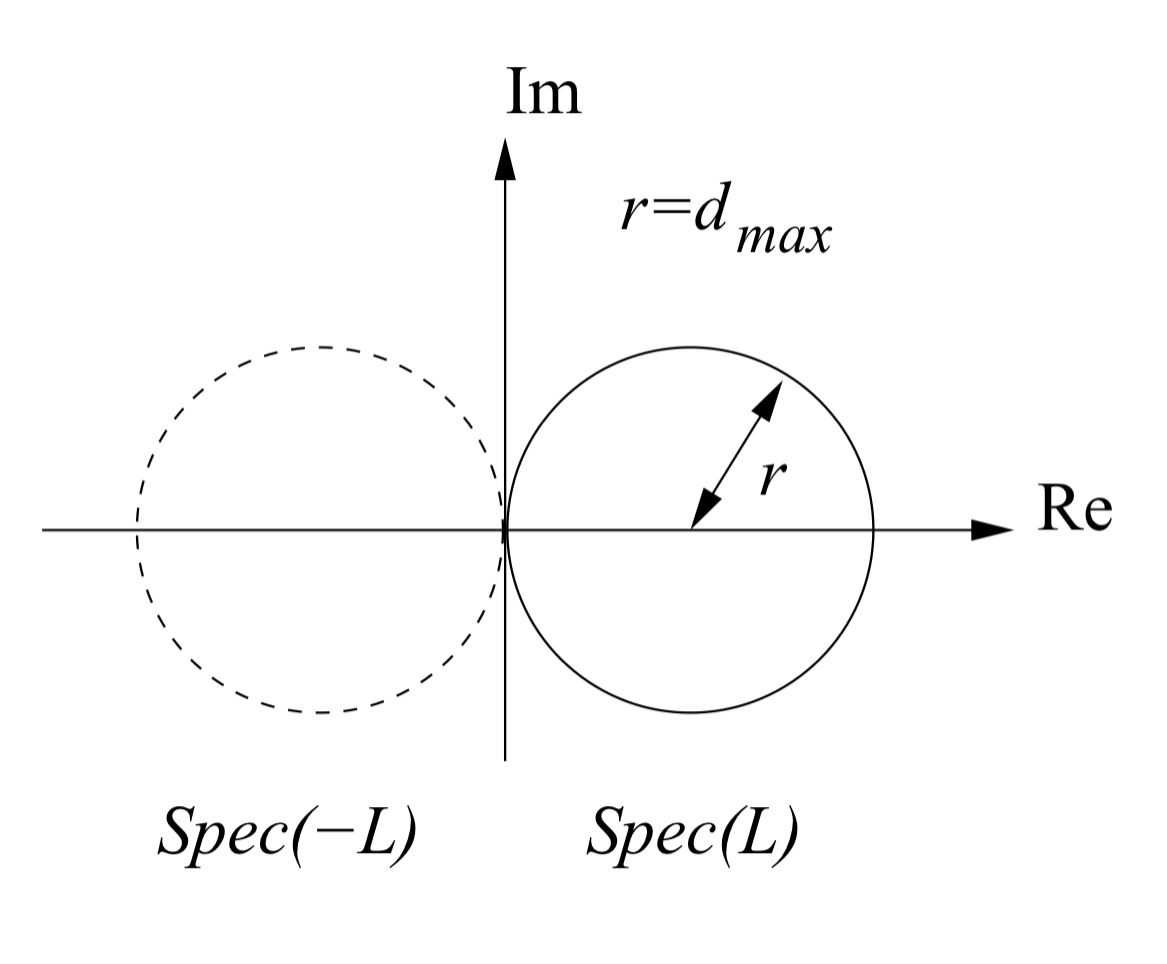
\includegraphics[width=8cm]{figures/Fig1-DiskTheorem.jpeg}
    \caption{A demonstration of Ger\v sgorin Theorem applied to graph Laplacian.}
    \label{DiskTheorem}
\end{figure}

{\color[gray]{0.5}
\noindent \textbf{Proof.}  Based on the Ger\v sgorin disk theorem, all the eigenvalues of $L=[l_{ij}]$ are located in the union of the following $n$ disks
}

\noindent \textbf{Proof.} 基于圆盘定理,所有$L=[l_{ij}]$的特征值都位于下面的$n$个圆盘的并集中

\begin{equation}
    D_i = \{ z\in \mathbb{C}: |z-l_{ii}| \le \sum_{j\in \mathcal{I},j\ne i}|l_{ij}| \}
    \tag{16}
    \label{16}
\end{equation}

{\color[gray]{0.5}
But $l_{ii} = \Delta_{ii}$ and
}

如果$l_{ii} = \Delta_{ii}$那么

\begin{equation}
    \sum_{j\in \mathcal{I},j\ne i}|l_{ij}|=\deg_{out}(v_i) = \Delta_{ii}
    \notag
\end{equation}

{\color[gray]{0.5}
\noindent Thus, $D_i = \{ z\in \mathbb{C}:|z - \Delta_{ii}| \le \Delta_{ii}\}$ . 
On the other hand, all these $n$ disks are contained in the largest disk $D(G)$ with radius $d_{max}(G)$. 
Clearly, all the eigenvalues of $−L$ are located in the disk $D^\prime(G)=\{ z\in \mathbb{C}: |z+d_{max}(G)|\le d_{max}(G)\}$ that is the mirror image of $D(G)$ with respect to the imaginary axis.
}

\noindent 因此,$D_i = \{ z\in \mathbb{C}:|z - \Delta_{ii}| \le \Delta_{ii}\}$。
另一方面,所有的$n$个圆盘被包含在一个最大的圆盘$D(G)$中,此圆盘半径为$d_{max}(G)$。
明显的,所有关于$-L$的特征值都位于$D(G)$关于虚轴镜像对阵的圆盘$D^\prime(G)=\{ z\in \mathbb{C}: |z+d_{max}(G)|\le d_{max}(G)\}$中。

{\color[gray]{0.5}
Here is an immediate corollary and the first convergence proof for protocol (A1) for a directed network.
}

以下是一个关于有向网络协议(\ref{A1})的直接推论和首次收敛证明。

{\color[gray]{0.5}
\noindent \textbf{Corollary 1.} Consider a network of integrators $\dot{x}_i = u_i$ where each node applies protocol (A1). 
Assume $G$ is a strongly connected digraph. 
Then, protocol (A1) globally asymptotically solves a consensus problem.
}

\noindent \textbf{Corollary 1.} 考虑一个积分器网络$\dot{x}_i = u_i$,每个节点都遵循协议(\ref{A1})。
假设图$G$是一个强连接图。
那么,协议(\ref{A1})能够全局解决渐进一致性问题。

{\color[gray]{0.5}
\noindent \textbf{Proof.} Since $G$ is strongly connected, $\text{rank}(L)=n-1$ and $L$ has a simple eigenvalue at zero. 
Based on Theorem 2, the rest of the eigenvalues of $−L$ have negative real-parts and therefore the linear system in (6) is stable. 
On the other hand, any equilibrium $x^*$ of (6) is a right eigenvector of $L$ associated with $\lambda=0$. 
Since the eigenspace associated with the zero eigenvalue is one-dimensional, there exists an $\alpha\in \mathbb{R}$ such that $x^*=\alpha\mathbf{1}$, i.e. $x^*=\alpha$ for all $i$.
}

\noindent \textbf{Proof.} 由于$G$是强连接图,$\text{rank}(L)=n-1$并且$L$有一个为0的特征值。
基于定理2(Theorem 2),$-L$余下的特征值有负实部,并且因此线性系统(\ref{6})是稳定的。
另一方面,系统(\ref{6})的任何平衡状态$x^*$都是一个$L$关于$\lambda=0$的右特征向量。
由于特征空间是与0特征值有联系的1维特征向量,这里存在一个$\alpha\in \mathbb{R}$使得$x^*=\alpha\mathbf{1}$,即对于所有的$i$都有$x^*=\alpha$。

{\color[gray]{0.5}
Keep in mind that Corollary 1 does not guarantee whether the decision value $\alpha$ of each node is equal to $\text{Ave}(x(0))$ or not. 
In other words, Corollary 1 does not necessarily address the average-consensus problem.
}

谨记推论1(Corollary 1)不能保证所有节点的决策值$\alpha$是否等于$\text{Ave}(x(0))$。
换句话说,推论1(Corollary 1)不一定能解决平均一致性问题。

% ------------------------------------------------------------------------------
\section{A Counterexample for Average-Consensus}
{\color[gray]{0.5}
\noindent A sufficient condition for the decision value $\alpha$ of each node in the proof of Corollary 1 to be equal to $\text{Ave}(x(0))$ is that $\sum_{i=1}^{n}u_i \equiv 0$. 
If $G$ is undirected (i.e. $a_{ij}=a_{ji} > 0,\forall i,j: a_{ij}\ne 0$), automatically the condition $\sum_{i=1}^{n}u_i=0$, $\forall x$ holds and $\text{Ave}(x(t))$ is an invariant quantity [20]. 
However, this property does not hold for a general digraph.
}

\noindent 在推论1(Corollary 1)协议中,所有节点的决策值$\alpha$等于$\text{Ave}(x(0))$的充分条件是$\sum_{i=1}^{n}u_i \equiv 0$。
如果图$G$是无向图(即$a_{ij}=a_{ji} > 0,\forall i,j: a_{ij}\ne 0$),自动的情况$\sum_{i=1}^{n}u_i=0$,$\forall x$和$\text{Ave}(x(t))$是不变的量,参考文献[20]。
然而,这个性质并不适用于一般有向图。

{\color[gray]{0.5}
A simple counterexample is a strongly connected digraph of order $n$ = 3, shown in Figure 2, with weights in \{0, 1\} and the following sets of vertices and edges:
}

一个简单的反例就是图(\ref{2})表示的3阶$n=3$强连接图,其中权重在\{0,1\}中,向量和边的集合如下所示:

\begin{equation}
    \mathcal{V} = \{1, 2, 3 \},\quad \mathcal{E}=\{12, 23, 31, 13\}.
    \notag
\end{equation}

\begin{figure}[htbp]
    \centering
    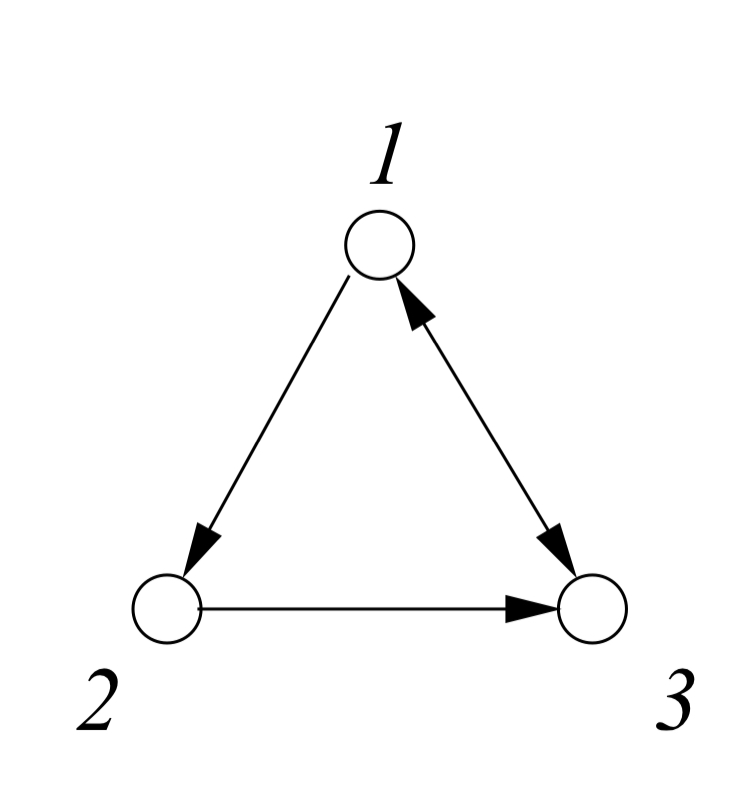
\includegraphics[width=4cm]{figures/Fig2-ConnectedDigraph.jpeg}
    \label{ConnectedDigraph}
    \caption{A connected digraph of order 3 that does not solve the average-consensus problem using Protocols (A1)}
\end{figure}

{\color[gray]{0.5}
For the digraph $G=(\mathcal{V}, \mathcal{E})$, $\sum_{i=1}^{3}u_i = x_3 - x_1$. 
Thus, if nodes 1 and 3 disagree, the property $\sum_{i=1}^{3}u_i = 0$ does not hold for all $x$. 
On the other hand, the reader can verify that for this example
}

对于图$G=(\mathcal{V}, \mathcal{E})$,$\sum_{i=1}^{3}u_i = x_3 - x_1$。
因此,如果节点1和3状态不相等,那么$\sum_{i=1}^{3}u_i = 0$不是对于所有的$x$都成立。
另一方面,读者可以在本例中来验证这一点

\begin{equation}
    L = \left[
    \begin{matrix}
        2 & -1 & -1 \\
        0 & 1 & -1 \\
        -1 & 0 & 1 
    \end{matrix}
    \right]
    \notag
\end{equation}

% {\color{userColor}
% \begin{equation}
%     D = \left[
%     \begin{matrix}
%         2 & 0 & 0 \\
%         0 & 1 & 0 \\
%         0 & 0 & 1 
%     \end{matrix}
%     \right],
%     A = \left[
%     \begin{matrix}
%         0 & 1 & 1 \\
%         0 & 0 & 1 \\
%         1 & 0 & 0 
%     \end{matrix}
%     \right],
%     L = D - A
%     \notag
% \end{equation}
% }

{\color[gray]{0.5}
\noindent and $x^*_i = [x_1(0) + x_2(0) + 2x_3(0)]/4$ (this is due to Theorem 3). 
This decision value is apparently in the convex hull of all the $x_i(0)$’s but it is different from $\text{Ave}(x(0))$ if and only if $x_1(0) + x_2(0) \ne 2x_3(0)$. 
As a result, for all initial conditions satisfying $x_1(0) + x_2(0) \ne 2x_3(0)$, Protocol (A1) does not solve the average-consensus problem but still all nodes reach an agreement. 
This motivates us to characterize the class of all digraphs that solve the average-consensus problem.
}

\noindent 并且$x^*_i = [x_1(0) + x_2(0) + 2x_3(0)]/4$(此公式源于Theorem 3)。
显而易见的这个决策值包含在所有$x_i(0)$的凸包中,但是当且仅当$x_1(0) + x_2(0) \ne 2x_3(0)$时,决策值不等于$\text{Ave}(x(0))$。
结果就是,对于所有满足$x_1(0) + x_2(0) \ne 2x_3(0)$的初始情况,协议(\ref{A1})并不能解决平均一致性问题,但所有的节点仍能达到一致。
这促使我们来描述所有的图的类,以解决平均一致性问题。

{\color[gray]{0.5}
Before presenting our first main result, we need to provide a limit theorem for exponential matrices of the form $e^{(-Lt)}$. 
This is because the solution of (6) is given by
}

在提出我们第一次的主要结果之前,我们需要提出一个指数矩阵如$e^{(-Lt)}$形式的极限理论。
这是因为公式(\ref{6})的解决办法是通过以下公式给出

\begin{equation}
    x(t) = exp(-Lt)x(0)
    \tag{17}
    \label{17}
\end{equation}

{\color[gray]{0.5}
\noindent and by explicit calculation of $exp(-Lt)$, we can obtain the decision value of each node after reaching consensus for a general digraph. 
The following theorem is closely related to a famous limit theorem in the theory of nonnegative matrices known as Perron-Frobenius Theorem [12].
}

\noindent 并且通过对$exp(-Lt)$的显示计算,我们可以得到普通图在达到一致性后每个节点的决策值。
接下来的定理在非负矩阵理论中与著名的极限定理关系密切,即Perron-Frobenius定理(Perron-Frobenius Theorem)[12]。

{\color[gray]{0.5}
\noindent \textbf{Notation.} Following the notation in [12], we denote the set of $m\times n$ real matrices by $M_{m,n}$  and the set of square $n\times n$ matrices by $M_n$ . 
Furthermore, throughout this paper, the right and left eigenvectors of the Laplacian $L$ associated with $\lambda_1 = 0$ are denoted by $w_r$ and $w_l$ , respectively.
}

\noindent \textbf{Notation.} 参考文献[12]的注解,我们记$M_{m,n}$为$m\times n$的实矩阵,$M_n$为$n \times n$的方阵。
进一步,通过这篇文章,关于$\lambda_1 = 0$的拉普拉斯矩阵$L$的右特征向量和左特征向量分别用$w_r$和$w_l$表示。

{\color[gray]{0.5}
\noindent \textbf{Theorem 3.} Assume $G$ is a strongly connected digraph with Laplacian $L$ satisfying $Lw_r=0$,$w_l^TL = 0$,$w_l^Tw_r=1$. Then
}

\noindent \textbf{Theorem 3.} 假设$G$是一个强连通图,拉普拉斯矩阵$L$满足$Lw_r=0$,$w_l^TL = 0$,$w_l^Tw_r=1$。那么

\begin{equation}
    R = \lim_{t\rightarrow +\infty} exp(-Lt) = w_r w_l^T \in M_n
    \tag{18}
    \label{18}
\end{equation}

% \begin{equation}
%     {\color{userColor} \text{R = t趋于无穷时-Lt关于e指数值极限 = 右特征向量 * 左特征向量}}
%     \notag
% \end{equation}

{\color[gray]{0.5}
\noindent \textbf{Proof.} Let $A=-L$ and let $J$ be the Jordan form associated with $A$, i.e. $A=SJS^{-1}$ . 
We have $exp(At) = S\ exp(Jt)\ S^{-1}$ and as $s\rightarrow +\infty$, $exp(Jt)$ converges to a matrix $Q=[q_{ij}]$ with a single nonzero element $q_{11}=1$. 
The fact that other blocks in the diagonal of $exp(Jt)$ vanish is due to the property that $Re(\lambda_k(A))<0$ for all $k\ge2$ where $\lambda_k(A)$ is the $k$th largest eigenvalue of $A$ in terms of magnitude $|\lambda_k|$ . 
Notice that $R=SQS^{-1}$ . 
Since $AS=SJ$ the first column of $S$ is $w_r$ . 
Similarly, $S^{-1}A = JS^{-1}$ that means the first row of $S^{-1}$ is $w_l^T$. 
Due to the fact that $S^{-1}S=I$, $w_l$ satisfies the property $w_l^Tw_r=1$ as stated in the question. 
A straightforward calculation shows that $R=w_rw_l^T\in M_n$.
}

\noindent \textbf{Proof.} 令$A=-L$,$J$为$A$的约当形,即$A=SJS^{-1}$。
我们有$exp(At) = S\ exp(Jt)\ S^{-1}$当$s\rightarrow +\infty$,$exp(Jt)$收敛至一个含有单一非零元素$q_{11}=1$的矩阵$Q=[q_{ij}]$。
对角矩阵$exp(Jt)$的其他块会变成0,由于对于所有的$k\ge2$,都有$Re(\lambda_k(A))<0$,这里$\lambda_k(A)$是矩阵$A$关于$|\lambda_k|$的第$k$个最大的特征值。
注意$R=SQS^{-1}$。
由于$AS=SJ$,$S$的第一列为$w_r$。
相似的,$S^{-1}A = JS^{-1}$,这也意味着$S^{-1}$的第一行是$w_l^T$。
由于$S^{-1}S=I$,$w_l$满足如问题中所述的性质$w_l^Tw_r=1$。
直接的计算显示$R=w_rw_l^T\in M_n$。

% ------------------------------------------------------------------------------
\section{Networks with Fixed or Switching Topology}
{\color[gray]{0.5}
\noindent In this section, we present three of our main results: 
i) characterization of all connected digraphs that solve average-consensus problem using Protocol (A1), 
and ii) the relation between the performance of Protocol (A1) and the Fiedler eigenvalue (i.e. algebraic connectivity) of graphs, 
and iii) robust agreement under switching topology due to link failure/creation.
}

\noindent 这部分,我们提出了三种主要的结果:i)描述了所有的连接图使用协议(\ref{A1})解决平均一致性的问题。
ii)协议(\ref{A1})的性能和图的费德勒特征值(即代数连通度)之间的联系。
iii)由于连接失效/新建的切换拓扑下的鲁棒一致性问题。

% ------------------------------------------------------------------------------
\subsection{Balanced Graphs and Average-Consensus on Digraphs}
{\color[gray]{0.5}
\noindent The following class of digraphs turns out to be instrumental in solving average-consensus problems:
}

\noindent 下述的图类表明了在解决一致性问题的分析:

{\color[gray]{0.5}
\noindent \textbf{Definition 1.} (balanced graphs) We say the node $v_i$ of a digraph $G=(\mathcal{V}, \mathcal{E}, \mathcal{A})$ is balanced if and only if its in-degree and out-degree are equal, i.e. $\deg_{out}(v_i)=\deg_{in}(v_i)$. 
A graph $G=(\mathcal{V}, \mathcal{E}, \mathcal{A})$ is called balanced if and only if all of its nodes are balanced, i.e. $\sum_{j}a_{ij} = \sum_{j}a_{ji}, \forall i$.
}

\noindent \textbf{Definition 1.} (平衡图)我们认为当且仅当图$G=(\mathcal{V}, \mathcal{E}, \mathcal{A})$的节点$v_i$的入度(in-degree)等于出度(out-degree)时,节点是平衡的,即$\deg_{out}(v_i)=\deg_{in}(v_i)$。
当图$G=(\mathcal{V}, \mathcal{E}, \mathcal{A})$的所有节点都是平衡时,图是平衡图,即$\sum_{j}a_{ij} = \sum_{j}a_{ji}, \forall i$。

{\color[gray]{0.5}
\noindent \textbf{Example 1.} Any undirected graph is balanced. Furthermore, the digraphs shown in Figure 3 are all balanced.
}

\noindent \textbf{Example 1.} 任意的无向图都是平衡的。
进一步说,图\ref{3}展示的图都是平衡的。

\begin{figure}[htbp]
    \centering
    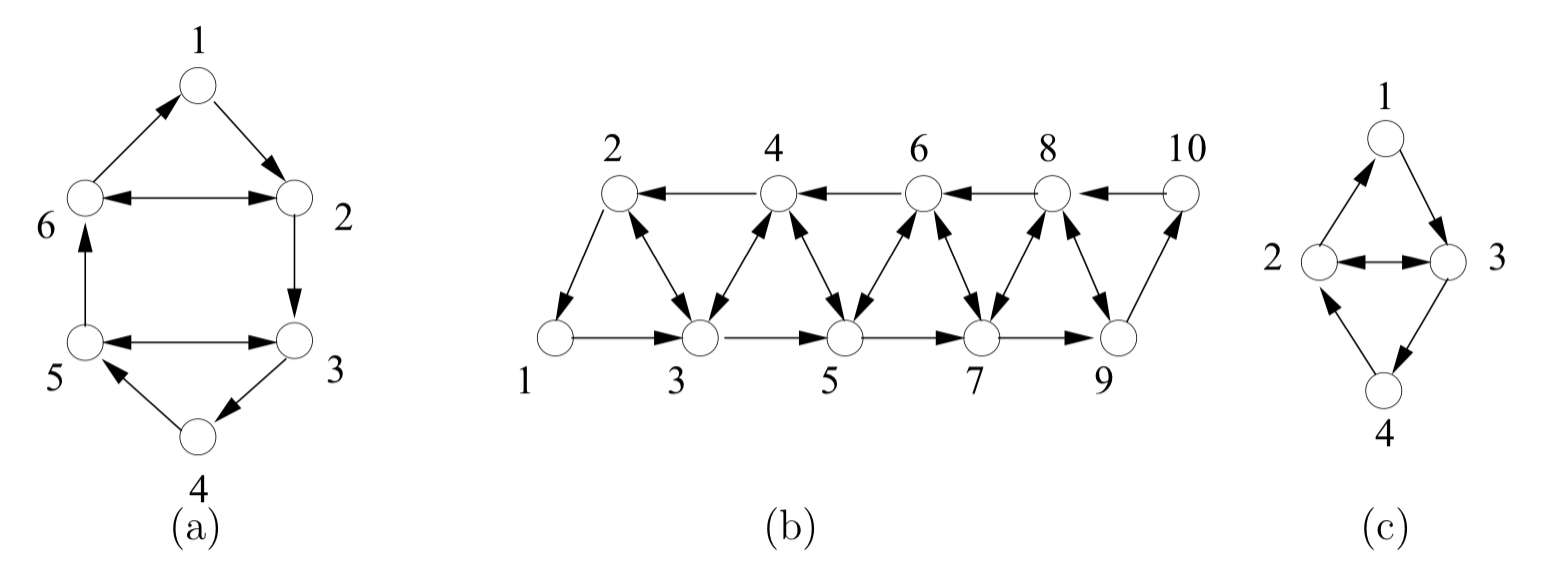
\includegraphics[width=12cm]{figures/Fig3-BalancedGraphs.jpeg}
    \label{BalancedGraphs}
    \caption{Three examples of balanced graphs.}
\end{figure}

{\color[gray]{0.5}
\noindent Here is our first main result:
}

\noindent 接下来是我们的第一个主要结论:

{\color[gray]{0.5}
\noindent \textbf{Theorem 4.} Consider a network of integrators with directed information flow $G=(\mathcal{V}, \mathcal{E}, \mathcal{A})$ that is strongly connected. 
Then, protocol (A1) globally asymptotically solves the average-consensus problem using if and only if $G$ is balanced.
}

\noindent \textbf{Theorem 4.} 考虑一个含有有向信息流$G=(\mathcal{V}, \mathcal{E}, \mathcal{A})$的积分器网络,网络是强连通的。
那么,当且仅当图$G$是平衡图时,协议(\ref{A1})全局渐进的解决了平均一致性问题。

{\color[gray]{0.5}
\noindent \textbf{Proof.} The proof follows from Theorems 5 and 6, below.
}

\noindent \textbf{Proof.} 证明参考如下定理5和定理6。

{\color[gray]{0.5}
\noindent {\em Remark} 5. According to Theorem 4, if a graph is not balanced, then protocol (A1) does not necessarily solve the average consensus-problem. This assertion is consistent with the counterexample given in Figure 2.
}

\noindent {\em Remark} 5. 根据定理4,如果图不是平衡图,那么协议(\ref{A1})没有办法解决平均一致性问题。
此断言与图\ref{ConnectedDigraph}给出的反例是一致的。

{\color[gray]{0.5}
\noindent \textbf{Theorem 5.} Consider a network of integrator agents with a digraph $G=(\mathcal{V}, \mathcal{E}, \mathcal{A})$ that is strongly connected. 
Then, protocol (A1) globally asymptotically solves the average-consensus problem if and only if $\mathbf{1}^TL=0$.
}

\noindent \textbf{Theorem 5.} 考虑一个积分器智能体网络图$G=(\mathcal{V}, \mathcal{E}, \mathcal{A})$是强连通的。
那么,当且仅当$\mathbf{1}^TL=0$时,协议(\ref{A1})全局渐进的解决了平均一致性问题。

{\color[gray]{0.5}
\noindent \textbf{Proof.} From Theorem 3, with $w_r = \frac{1}{\sqrt{n}}\mathbf{1}$ we obtain 
}

\noindent \textbf{Proof.} 参考定理3,当$w_r = \frac{1}{\sqrt{n}}\mathbf{1}$时我们有

\begin{equation}
    x^* = \lim_{t\rightarrow +\infty}x(t) = Rx_0 = w_r(w_l^T x_0) = \frac{1}{\sqrt{n}}(w_l^Tx_0)\mathbf{1}
    \notag
\end{equation}

{\color[gray]{0.5}
\noindent This implies Protocol 1 globally exponentially solves a consensus problem with the decision value $\frac{1}{\sqrt{n}}(w_l^Tx_0)$ for each node. 
If this decision value is equal to $Ave(x_0), \forall x_0 \in \mathbb{R}^n$ , then necessarily $\frac{1}{\sqrt{n}}w_l = \frac{1}{\sqrt{n}}$ , i.e. $w_l= w_r=\frac{1}{\sqrt{n}}\mathbf{1}$. 
This implies that $\mathbf{1}$ is the left eigenvector of $L$. 
To prove the converse, assume that $\mathbf{1}^TL=0$. 
Let us take $w_r=\frac{1}{\sqrt{n}}\mathbf{1}$, $w_l=\beta\mathbf{1},$ with $\beta\in\mathbb{R},\beta\ne0$. 
From condition $w_l^Tw_r=1$, we get $\beta=\frac{1}{\sqrt{n}}$ and $w_l=\frac{1}{\sqrt{n}}\mathbf{1}$. 
This means that the decision value for every node is $\frac{1}{\sqrt{n}}(w_l^Tx_0)=\frac{1}{n}\mathbf{1}^Tx_0=Ave(x_0)$.
}

\noindent 这表明协议1全局指数解决了每一个节点关于决策值$\frac{1}{\sqrt{n}}(w_l^Tx_0)$的一致性问题。
如果这个决策值等于$Ave(x_0), \forall x_0 \in \mathbb{R}^n$,那么必要的$\frac{1}{\sqrt{n}}w_l = \frac{1}{\sqrt{n}}$,即$w_l= w_r=\frac{1}{\sqrt{n}}\mathbf{1}$。
这表明$\mathbf{1}$是关于$L$的左特征向量。
为了证明一致性,假设$\mathbf{1}^TL=0$。
我们令$w_r=\frac{1}{\sqrt{n}}\mathbf{1}$,$w_l=\beta\mathbf{1},\beta\in\mathbb{R},\beta\ne0$。
根据条件$w_l^Tw_r=1$,我们得到$\beta=\frac{1}{\sqrt{n}}$和$w_l=\frac{1}{\sqrt{n}}\mathbf{1}$。
这意味着每一个节点的决策值是$\frac{1}{\sqrt{n}}(w_l^Tx_0)=\frac{1}{n}\mathbf{1}^Tx_0=Ave(x_0)$。

{\color[gray]{0.5}
\noindent \textbf{Corollary 2.} Assume all the conditions in Theorem 5 hold. 
Suppose $L$ has a left eigenvector $\gamma = (\gamma_1, \dots, \gamma_n)^T$ associated with $\lambda=0$ that is a nonnegative vector in $\mathbb{R}^n$ (i.e. a vector with non-negative elements) satisfying $\sum_i\gamma_i>0$. 
Then, the group decision value after reaching consensus is given by
}

\noindent \textbf{Corollary 2.} 假设定理5中的所有条件成立。
假设$L$有一个关于特征值$\lambda=0$的左特征向量$\gamma = (\gamma_1, \dots, \gamma_n)^T$,此特征向量是一个属于$\mathbb{R}^n$的非负向量(即向量元素非负)且满足$\sum_i\gamma_i>0$。
那么,群组达到一致的决策值就是:

\begin{equation}
    \alpha = \frac{\sum_i \gamma_ix_i(0)}{\sum_i\gamma_i}
    \tag{19}
    \label{19}
\end{equation}

{\color[gray]{0.5}
\noindent i.e. the decision value is in the convex hull of initial values of the nodes.
}

\noindent 即决策值包含在在节点初始值的凸包中。

{\color[gray]{0.5}
\noindent \textbf{Proof.} We have $\gamma^TL=0$ and thus $\gamma^Tu\equiv0$ (because $u=-Lx$). 
Therefore, $\beta=\gamma^Tx$ is an invariant quantity. 
Assume, the digraph $G$ is not balanced. 
Then, still an agreement is asymptotically reached. 
Let $\alpha$ be the decision value of all nodes after reaching consensus. 
We have $\gamma^Tx^*=\gamma^Tx(0)$ due to invariance of $\gamma^Tx(0)$. 
But $x^*=\alpha\mathbf{1}$, thus we obtain
}

\noindent \textbf{Proof.} 
我们有$\gamma^TL=0$那么因此$\gamma^Tu\equiv0$(因为$u=-Lx$)的集合。
因此,$\beta=\gamma^Tx$是一个不变的量。
假如,图$G$是不平衡的。
那么,一致性仍是渐进达到的。
定义$\alpha$是所有节点达到一致后的决策值。
我们有$\gamma^Tx^*=\gamma^Tx(0)$由于$\gamma^Tx(0)$是不变的。
但是$x^*=\alpha\mathbf{1}$,因此我们得到

\begin{equation}
    (\sum_i\gamma_i)\alpha = \gamma^Tx(0)
    \notag
\end{equation}

{\color[gray]{0.5}
\noindent and the result follows.
}

\noindent 结果如下。

{\color[gray]{0.5}
The following result shows that if one of the agents uses a relatively small update rate (or step-size), i.e. $\gamma_{i^*}\gg\gamma_i$ for all $i\ne i^*$. 
Then, the value of all nodes converges to the value of $x_{i^*}$. 
In other words, the agent $i^*$ plays the role of a leader in leader-follower type architecture.
}

接下来的结果表明,如果一个智能体使用了一个相当小的更新速率(或step-size),即$\gamma_{i^*}\gg\gamma_i$对于所有的$i\ne i^*$。
那么,所有节点的决策值收敛至$x_{i^*}$。
换句话说,智能体$i^*$在领导者跟随(leader-follower)类型结构中扮演领导者的角色。

{\color[gray]{0.5}
\noindent \textbf{Corollary 3.} (multi-rate integrators) Consider a network of multi-rate integrators with the node dynamics
}

\noindent \textbf{Corollary 3.} (多比例积分)考虑一个多比例积分网络,其节点动态如下:

\begin{equation}
    \gamma_i \dot{x}_i=u_i,\quad \gamma_i>0,\forall i \in \mathcal{I}
    \tag{20}
    \label{20}
\end{equation}

{\color[gray]{0.5}
\noindent Assume each node applies Protocol (A1). 
Then, an agreement is globally asymptotically reached and the decision value of the group is
}

\noindent 假设每一个节点满足协议(\ref{A1})。
那么,达到一致的群组决策值就是:

\begin{equation}
    \alpha = \frac{\sum_i \gamma_ix_i(0)}{\sum_i\gamma_i}
    \tag{21}
    \label{21}
\end{equation}

{\color[gray]{0.5}
\noindent \textbf{Proof.} The dynamics of the network evolves according to
}

\noindent \textbf{Proof.} 网络根据下式动态变化:

\begin{equation}
    D\dot{x} = -Lx
    \notag
\end{equation}

{\color[gray]{0.5}
\noindent where $D=diag(\gamma)$ is a diagonal matrix with the $i$th diagonal element that is equal to $\gamma_i>0$. 
The last equation can be rewritten as
}

\noindent 这里,$D=diag(\gamma)$是具有第$i$个对角元素的对角矩阵,对角元素满足$\gamma_i>0$。
上边的公式可以改写为:

\begin{equation}
    \dot{x} = -\tilde{L}x
    \notag
\end{equation}

{\color[gray]{0.5}
\noindent where $\tilde{L} = D^{-1}L = diag(\frac{1}{\gamma_1},\dots,\frac{1}{\gamma_n})L$ is a valid Laplacian matrix for a digraph $\tilde{G}$ with adjacency matrix $\tilde{A}=D^{-1}\mathcal{A}$ (i.e. the weights of the edges leaving node $i$ are divided by $\gamma_i$ ). 
Clearly, $\gamma$ is a vector with positive elements that is the left eigenvector of $\tilde{L}$ and based on Corollary 2 the decision value is in the weighted average of $x_i(0)$’s with weights specified by $\gamma$ .
}

\noindent 这里,$\tilde{L} = D^{-1}L = diag(\frac{1}{\gamma_1},\dots,\frac{1}{\gamma_n})L$是图$\tilde{G}$和邻接矩阵$\tilde{A}=D^{-1}\mathcal{A}$(即从节点$i$出发的边的权重被$\gamma_i$分割)的拉普拉斯矩阵。
清晰的,$\gamma$是一个正元素向量,它是$\tilde{L}$的左特征向量,并且基于推论2决策值是位于被$x_i(0)$的平均权重中被$\gamma$整除。

{\color[gray]{0.5}
\noindent {\em Remark} 6. The discrete-time model and attitude alignment protocol discussed in Jadbabaie et al. [13] correspond to the first-order Euler approximation of equation (20) with protocol (A1) and the special choice of $\gamma_i=deg_{out}(v_i)+1$ in Corollary 3. 
In [6], a Laplacian matrix is defined as $I-D\mathcal{A}$ which in the context of this paper is equivalent to a multi-rate network of integrators with $\gamma_i=deg_{out}(v_i)\ge 0$. 
The singularity of $D$ that is caused by the choice of $\gamma_i=deg_{out}(v_i)$ is avoided in [13] by properly adding a positive constant (e.g. 1) to $deg_{out}(v_i)$.
}

\noindent {\em Remark} 6. Jadbabaie等[13]人讨论了关于公式(\ref{20})和协议(\ref{A1})的一阶Euler渐进(Euler approximation)离散时间模型和姿态位置协议,以及推论3中的特殊选择$\gamma_i=deg_{out}(v_i)+1$。
在文献[6],拉普拉斯矩阵被定义为$I-D\mathcal{A}$,在本文中这等价于一个$\gamma_i=deg_{out}(v_i)\ge 0$多比例积分网络。
$D$的奇异性由$\gamma_i=deg_{out}(v_i)$的选择决定,这在文献[13]中通过增加合适的正常量(即1)到$deg_{out}(v_i)$上来避免。

{\color[gray]{0.5}
\noindent \textbf{Theorem 6.} Let $G=(\mathcal{V}, \mathcal{E}, \mathcal{A})$ be a digraph with an adjacency matrix $\mathcal{A}=[a_{ij}]$. 
Then, all the following statements are equivalent:

i) G is balanced, 

ii) $w_l = \mathbf{1}$ is the left eigenvector of the Laplacian of $G$ associates with the zero eigenvalue, i.e. $\mathbf{1}^TL = 0$.

iii) $\sum_{i=1}^n u_i = 0$, $\forall x \in \mathbb{R}^n$ with $u_i = \sum_{j\in N_i}a_{ij}(x_j - x_i)$.
}

\noindent \textbf{Theorem 6.} 定义一个具有邻接矩阵$\mathcal{A}=[a_{ij}]$的图$G=(\mathcal{V}, \mathcal{E}, \mathcal{A})$。
那么,下列所有的条件都是等价的:

i)图$G$是平衡的;

ii)$w_l = \mathbf{1}$是图$G$拉普拉斯矩阵相对于0特征值的左特征向量,即$\mathbf{1}^TL = 0$。

iii)对$\forall x \in \mathbb{R}^n$有$\sum_{i=1}^n u_i = 0$,且$u_i = \sum_{j\in N_i}a_{ij}(x_j - x_i)$。

{\color[gray]{0.5}
\noindent \textbf{Proof.} We show i) $\Leftrightarrow$ ii) and ii) $\Leftrightarrow$ iii).
}

\noindent \textbf{Proof.} 我们证明了i)$\Leftrightarrow$ ii)和ii)$\Leftrightarrow$ iii)。

{\color[gray]{0.5}
Proof of i) $\Leftrightarrow$ ii): We have $\Delta_{ii} = deg_{out}(v_i)$ and $deg_{in}(v_i)=\sum_{j,j\ne i}a_{ji}$, thus the $i$th column sum of $L$ is equal to
}

关于i)$\Leftrightarrow$ ii)的证明:
我们有$\Delta_{ii} = deg_{out}(v_i)$和$deg_{in}(v_i)=\sum_{j,j\ne i}a_{ji}$,因此矩阵$L$第$i$列的和等于

\begin{equation}
    \sum_il_{ji} = \sum_{i,j\ne i}l_{ji}+l_{ii} = -deg_{in}(v_i) + deg_{out}(v_i) = 0 \Leftrightarrow \text{图}G\text{的节点}v_i\text{是平衡的}
    \notag
\end{equation}

{\color[gray]{0.5}
\noindent Noting that the $i$ column sum of $L$ is the same as the $i$th element of the row vector $\mathbf{1}^TL$, one concludes that $\mathbf{1}^TL=0$ iff all the nodes of $G$ are balanced, i.e. $G$ is balanced.
}

\noindent 注意到矩阵$L$第$i$列的和等于向量$\mathbf{1}^TL$的第$i$个行元素,可以断定当且仅当图$G$的所有节点是平衡的,即图$G$是平衡的,有$\mathbf{1}^TL=0$。

{\color[gray]{0.5}
Proof of ii) $\Leftrightarrow$ iii): 
Since $u=-Lx$, ($\sum_iu_i=0,\forall x$) $\Leftrightarrow$ ($\mathbf{1}^Tu=-(\mathbf{1}^TL)x=0, \forall x$) $\Leftrightarrow$ $\mathbf{1}^TL=0$.
}

对于ii)$\Leftrightarrow$ iii)的证明:
由于$u=-Lx$,($\sum_iu_i=0,\forall x$)$\Leftrightarrow$ ($\mathbf{1}^Tu=-(\mathbf{1}^TL)x=0, \forall x$)$\Leftrightarrow$ $\mathbf{1}^TL=0$。

{\color[gray]{0.5}
\noindent {\em Remark} 7. Notice that in Theorem 6, the graph $G$ does not need to be connected.
}

\noindent {\em Remark} 7. 注意在定理6中,图$G$不需要连通。

% ------------------------------------------------------------------------------
\subsection{Performance of Group Agreement and Mirror Graphs}
{\color[gray]{0.5}
\noindent In this section, we discuss performance issues of Protocol (A1) with balanced graphs. 
An important consequence of Theorem 6 is that for networks with balanced information flow, $\alpha = Ave(x)$ is an invariant quantity. 
This is certainly not true for an arbitrary digraph. 
The invariance of $Ave(x)$ allows decomposition of $x$ according to the following equation:
}

\noindent 在这部分,我们讨论平衡图的协议(\ref{A1})性能的一些问题。
定理6的一个重要的结果就是对于平衡信息流网络而言,$\alpha = Ave(x)$是一个不变的量。
对于任意的有向图,并不是确定正确的。
$Ave(x)$的不变性允许$x$的进行以下分解:

\begin{equation}
    x = \alpha \mathbf{1} + \delta
    \tag{22}
    \label{22}
\end{equation}

{\color[gray]{0.5}
\noindent where $\alpha = Ave(x)$ and $\delta\in \mathbb{R}^n$ satisfies $\sum_i\delta_i=0$. 
We refer to $\delta$ as the (group) disagreement vector. 
The vector $\delta$ is orthogonal to $\mathbf{1}$ and belongs to an $(n-1)$-dimensional subspace called the disagreement eigenspace of $L$ provided that $G$ is strongly connected. 
Moreover, $\delta$ evolves according to the (group) disagreement dynamics given by
}

\noindent 这里,$\alpha = Ave(x)$,$\delta\in \mathbb{R}^n$且满足$\sum_i\delta_i=0$。
我们引用$\delta$作为(群组)非一致向量。
向量$\delta$与$\mathbf{1}$正交,且属于一个$(n-1)$-维子空间,此子空间叫做强连通图$G$的拉普拉斯矩阵$L$的非一致特征空间。
此外,$\delta$还根据下边的(群组)非一致公式动态变化

\begin{equation}
    \dot{\delta} = -L\delta
    \tag{23}
    \label{23}
\end{equation}

{\color[gray]{0.5}
Define the Laplacian disagreement function of a digraph $G$ as
}

定义图$G$的拉普拉斯矩阵非一致函数为:

\begin{equation}
    \Phi_G(x) = x^T Lx
    \tag{24}
    \label{24}
\end{equation}

{\color[gray]{0.5}
\noindent with $L=\mathcal{L}(G)$. 
For digraphs, $\Phi_G(x)$ can be negative (e.g. the Laplacian of a digraph with two nodes and a single edge 12 is not positive semidefinite).
}

\noindent 这里$L=\mathcal{L}(G)$。
对于图,$\Phi_G(x)$可以是负定的(例如,两个节点和一个边12的图拉普拉斯矩阵是非半正定的)。

{\color[gray]{0.5}
It turns out that a useful property of balanced digraphs is that their Laplacian disagreement function is positive semidefinite. 
In addition, for any balanced digraph $G$, there exists an undirected graph that has the same Laplacian disagreement function as $G$. 
In the following, we formally define this induced undirected graph.
}

平衡图的一个有用性质是,它们的拉普拉斯矩阵非一致函数是半正定的。
另外,对于任意的平衡图$G$,都存在一个具有相同拉普拉斯非一致函数的无向图$G$。
接下来,我们正式定义这个感应无向图。

{\color[gray]{0.5}
\noindent \textbf{Definition 2.} (mirror graph/operation) Let $G=(\mathcal{V}, \mathcal{E}, \mathcal{A})$ be weighted digraph. 
Let $\tilde{\mathcal{E}}$ be the set of reverse edges of $G$ obtained by reversing the order of nodes of all the pairs in $\mathcal{E}$. 
The mirror of $G$ denoted by $\hat{G}=\mathcal{M}(G)$ is an undirected graph in the form $\hat{G}=(\mathcal{V}, \hat{\mathcal{E}}, \hat{\mathcal{A}})$ with the same set of nodes as $G$, the set of edges $\hat{\mathcal{E}}=\mathcal{E}\cup \tilde{\mathcal{E}}$, and the symmetric adjacency matrix $\hat{\mathcal{A}}=[\hat{a}_{ij}]$ with elements
}

\noindent \textbf{Definition 2.} (镜像图/操作)定义加权有向图$G=(\mathcal{V}, \mathcal{E}, \mathcal{A})$。
定义$\tilde{\mathcal{E}}$是图$G$的反转边的一部分,图$G$通过反转$\mathcal{E}$中所有成对节点的顺序得到。
图$G$的镜像定义为$\hat{G}=\mathcal{M}(G)$,它是一个形式为$\hat{G}=(\mathcal{V}, \hat{\mathcal{E}}, \hat{\mathcal{A}})$的无向图,具有和$G$一样的节点,边$\hat{\mathcal{E}}=\mathcal{E}\cup \tilde{\mathcal{E}}$,和渐进邻接矩阵$\hat{\mathcal{A}}=[\hat{a}_{ij}]$元素为

\begin{equation}
    \hat{a}_{ij}=\hat{a}_{ji}=\frac{a_{ij}+a_{ji}}{2}\ge 0
    \tag{25}
    \label{25}
\end{equation}

{\color[gray]{0.5}
The following result shows that the operations of $\mathcal{L}$ and $Sym$ on a weighted adjacency matrix $\mathcal{A}$ commute.
}

接下来的结果展示了关于$\mathcal{L}$和在加权邻接矩阵$\mathcal{A}$进行交换时的符号操作。

{\color[gray]{0.5}
\noindent \textbf{Theorem 7.} Let $G$ be a digraph with adjacency matrix $\mathcal{A}=adj(G)$ and Laplacian $L=\mathcal{L}(G)$. 
Then $L_s = Sym(L) = (L+L^T)/2$ is a valid Laplacian matrix for $\hat{G}=\mathcal{M}(G)$ if and only if $G$ is balanced, i.e. the following diagram commutes iff $G$ is balanced
}

\noindent \textbf{Theorem 7.} 定义$G$是一个具有邻接矩阵$\mathcal{A}=adj(G)$和拉普拉斯矩阵$L=\mathcal{L}(G)$的图。
那么当且仅当$G$是平衡图时,$L_s = Sym(L) = (L+L^T)/2$是一个关于$\hat{G}=\mathcal{M}(G)$的有效拉普拉斯矩阵,即有下述转换形式

\begin{equation}
    \begin{aligned}
                    &G \xrightarrow{adj}         &\mathcal{A} \xrightarrow{\mathcal{L}}          &L \\
        \mathcal{M} &\downarrow \quad\quad Sym   &\downarrow  Sym                      &\downarrow \\
                    &\hat{G} \xrightarrow[adj]{} &\hat{\mathcal{A}} \xrightarrow[\mathcal{L}]{}  &\hat{L} 
    \end{aligned}
    \tag{26}
    \label{26}
\end{equation}

{\color[gray]{0.5}
\noindent Moreover, if $G$ is balanced, the Laplacian disagreement functions of $G$ and $\hat{G}$ are equal.
}

\noindent 此外,如果$G$是平衡图,那么$G$的拉普拉斯非一致函数和$\hat{G}$是相等的。

{\color[gray]{0.5}
\noindent\textbf{Proof.} We know that $G$ is balanced iff $\textbf{1}^TL=0$. 
Since $L\textbf{1}=0$, we have $\mathbf{1}^TL=0$ $\Leftrightarrow$ $\frac{1}{2}(L+L^T)\mathbf{1}=0$. 
Thus, $G$ is balanced iff $L_s$ has a right eigenvector of $\mathbf{1}$ associated with $\lambda=0$, i.e. $L_s$ is a valid Laplacian matrix.
Now, we prove that $L_s=\mathcal{L}(\hat{G})$. 
For doing so, let us calculate $\hat{\Delta}$ element-wise, we get
}

\noindent\textbf{Proof.} 我们知道当且仅当$\textbf{1}^TL=0$时图$G$是平衡的。
由于$L\textbf{1}=0$,我们有$\mathbf{1}^TL=0$ $\Leftrightarrow$ $\frac{1}{2}(L+L^T)\mathbf{1}=0$。
因此当且仅当$L_s$有一个特征值是$\lambda=0$的右特征向量$\mathbf{1}$时,$G$是平衡的,即$L_s$是一个有效的拉普拉斯矩阵。
现在,我们证明$L_s=\mathcal{L}(\hat{G})$。
为了证明,我们计算$\hat{\Delta}$的元素,可以得到:

\begin{equation}
    \hat{\Delta}_{ii}=\sum_j \frac{a_{ij}+a_{ji}}{2}=\frac{1}{2}(deg_{out}(v_i)+deg_{in}(v_i))=deg_{out}(v_i)=\Delta_{ii}
    \notag
\end{equation}

{\color[gray]{0.5}
\noindent Thus, $\hat{\Delta}=\Delta$. 
On the other hand, we have
}

\noindent 因此,$\hat{\Delta}=\Delta$。
另一方面,我们有

\begin{equation}
    L_s = \frac{1}{2}(L+L^T) = \Delta-\frac{A+A^T}{2}=\hat{\Delta}-\hat{A}=\hat{L}=\mathcal{L}(\hat{G})
    \notag
\end{equation}

{\color[gray]{0.5}
\noindent The last part simply follows from the fact that $\hat{L}$ is equal to the symmetric part of $L$ and $x^T(L-L^T)x\equiv0$.
}

\noindent 最后一部分来源于$\hat{L}$等于$L$的渐进部分,且$x^T(L-L^T)x\equiv0$。

{\color[gray]{0.5}
\noindent\textbf{Notation.} For simplicity of notation, in the context of algebraic graph theory, $\lambda_k(G)$ is used to denote $\lambda_k(\mathcal{L}(G))$.
}

\noindent\textbf{Notation.} 为了简化符号,在代数图论部分,用$\lambda_k(G)$来表示$\lambda_k(\mathcal{L}(G))$。

{\color[gray]{0.5}
Now, we are ready to present our main result on performance of the Protocol (A1) in terms of the speed of reaching a consensus as a group.
}

现在,我们准备演示对协议(\ref{A1})关于群组达到一致性的速度的研究结果。

{\color[gray]{0.5}
\noindent\textbf{Theorem 8.} (performance of agreement) Consider a network of integrators with a directed information flow $G$ that is balanced and strongly connected. 
Then, given Protocol (A1), the following statements hold:
}

\noindent\textbf{Theorem 8.} (一致性的性能)考虑带有有向信息流$G$是平衡和强连通的积分器网络。
那么,给出协议(\ref{A1}),下述状态满足:

{\color[gray]{0.5}
i) the group disagreement (vector) $\delta$ as the solution of the disagreement dynamics in (23) globally asymptotically vanishes with a speed that is equal to $\kappa=\lambda_2(\hat{G})$ (or the Fiedler eigenvalue of the mirror graph of $G$), i.e.
}

i)群组的非一致向量$\delta$是非一致变化在公式(\ref{23})全局渐进消失的结果,消失速度等于$\kappa=\lambda_2(\hat{G})$(或图$G$镜像的费德勒特征值),即

\begin{equation}
    \tag{27}
    \label{27}
    ||\delta(t)||\le ||\delta(0)||exp(-kt)
\end{equation}

{\color[gray]{0.5}
ii) the following smooth, positive definite, and proper function
}

ii)下述的流畅的,正定的,适当的函数

\begin{equation}
    \tag{28}
    \label{28}
    V(\delta) = \frac{1}{2}||\delta||^2
\end{equation}

{\color[gray]{0.5}
is a valid Lyapunov function for the disagreement dynamics.
}

是一个关于非一致动态变化的有效李亚普诺夫函数。

{\color[gray]{0.5}
\noindent\textbf{Proof.} We have
}

\noindent\textbf{Proof.} 我们有

\begin{equation}
    \tag{29}
    \label{29}
    \dot{V} = -\delta^TL\delta = -\delta^TL_s\delta = -\delta^T\hat{L}\delta \le -\lambda_2(\hat{G})||\delta||^2 = -2\kappa V(\delta) < 0, \forall \delta \ne 0
\end{equation}

{\color[gray]{0.5}
\noindent This proves that $V(\delta)$ is a valid Lyapunov function for the group disagreement dynamics. 
Moreover, $\delta(t)$ vanishes globally exponentially fast with a speed of $\kappa$ as $t\rightarrow +\infty ..$ 
The fact that $L_s = \hat{L}$ is a valid Laplacian matrix for an undirected graph (i.e. mirror of $G$) follows from Theorem 7 and the inequality
}

\noindent 这证明$V(\delta)$是一个关于群组动态非一致的有效李亚普诺夫函数。
此外,$\delta(t)$全局指数消失随着$t\rightarrow +\infty .$速度为$\kappa$。
事实上$L_s = \hat{L}$是一个关于无向图(即$G$的镜像)的有效拉普拉斯矩阵,来源于定理7且有不相等性

\begin{equation}
    \tag{30}
    \label{30}
    \delta^T \hat{L} \delta \ge \lambda_2(\hat{G})||\delta||^2,\quad \forall\delta:\mathbf{1}^T\delta=0
\end{equation}

{\color[gray]{0.5}
\noindent which is due to equation (14).
}

\noindent 这来源于公式(\ref{14})。

{\color[gray]{0.5}
A well-known observation regarding the Fiedler eigenvalue of an undirected graph is that for dense graphs $\lambda_2$ is relatively large and for sparse graphs $\lambda_2$ is relatively small [11] (this is why $\lambda_2$ is called the algebraic connectivity). 
According to this observation, from Theorem 8, one can conclude that a network with dense interconnections solves an agreement problem faster than a connected but sparse network. 
This is consistent with common sense regarding agreement in a group. 
As a special case, a cycle of length $n$ that creates a balanced digraph on $n$ nodes solves an agreement problem. 
However, this is a relatively slow way to solve such a consensus problem.
}

一个关于无向图费德勒特征值众所周知的知识,对于密集图$\lambda_2$是相当大的,而对于稀疏图$\lambda_2$是相当小的[11](这是为什么$\lambda_2$被叫做代数连通度)。
根据这个情况,结合定理8,可以推断一个具备内部密集连接的网络比一个内部稀疏连接的网络能更快的解决一致性问题。
这和群组一致性问题具有一致的现象。
特殊的,一个由长度为$n$的环创造出的具备$n$节点的平衡图,可以解决一致性问题。
然而,这是一种很慢的解决一致性问题的方式。

% ------------------------------------------------------------------------------
\subsection{Consensus in Networks with Switching Topology}
{\color[gray]{0.5}
\noindent Consider a network of mobile agents that communicate with each other and need to agree upon a certain objective of interest or perform synchronization. 
Since, the nodes of the network are moving, it is not hard to imagine that some of the existing communication links can fail simply due to the existence of an obstacle between two agents. 
The opposite situation can arise where new links between nearby agents are created because the agents come to an effective range of detection with respect to each other. 
In other words, in the graph $G$ representing the information flow of the network, certain edges can be added or removed from $G$. 
Here, we are interested to investigate that in case of a network with switching topology whether it is still possible to reach a consensus or not.
}

\noindent 考虑一个节点间互相沟通的移动智能体网络,需要一致到一个感兴趣的目标或表现同步。
由于网络节点一直在移动,不难猜想,由于两个智能体之间存在障碍物,通信连接很容易丢失。
由于智能体进入了其他智能体的有效检测范围,那么就会发生相邻智能体之间出现新连接的相反情况。
换句话说,在用图$G$表示的有限信息流网络中,图$G$的某些边缘会增加或移除。
在这里,我们致力于发现探索网络具有切换拓扑的情况,无论是否能够达到一致性。

{\color[gray]{0.5}
Consider a hybrid system with a continuous-state $x \in \mathbb{R}^n$ nand a discrete-state $G$ that belongs to a finite set of digraphs
}

考虑一个具有连续状态$x \in \mathbb{R}^n$和离散状态$G$的混合系统,这属于图的一个有限集合

\begin{equation}
    \Gamma_n = \{ G: G\ \text{is a digraph of order}\ n\ \text{that is}\ strongly\ connected\ \text{and}\ balanced \}
    \notag
\end{equation}

{\color[gray]{0.5}
\noindent that can be analytically expressed in the form
}

\noindent 可以被分析表示成如下形式:

\begin{equation}
    \Gamma_n = \{ G=(\mathcal{V}, \mathcal{E}, \mathcal{A}): \text{rank}(\mathcal{L}(G)) =n-1, \mathbf{1}^T\mathcal{L}(G) = 0\}
    \tag{31}
    \label{31}
\end{equation}

{\color[gray]{0.5}
\noindent Given the node dynamics and protocol, the continuous-state of the system evolves according to the following dynamics
}

\noindent 给出节点的动态变化协议,那么系统的连续状态根据如下公式变化:

\begin{equation}
    \dot{x}(t) = -\mathcal{L}(G_k)x(t),\quad k=s(t), G_k\in \Gamma_n
    \tag{32}
    \label{32}
\end{equation}

{\color[gray]{0.5}
\noindent where $s(t): \mathbb{R}_{\ge 0}\rightarrow \mathcal{I}_{\Gamma_n}$ is a switching signal and $\mathcal{I}_{\Gamma_n}\subset \mathbb{N}$ is the index set associated with the elements of $\Gamma_n$. 
Clearly, $\Gamma_n$ is a finite set, because either a digraph has no edges or it is a complete graph with $n(n-1)$ directed edges.
}

\noindent 这里,$s(t): \mathbb{R}_{\ge 0}\rightarrow \mathcal{I}_{\Gamma_n}$是切换信号(switching signal),并且$\mathcal{I}_{\Gamma_n}\subset \mathbb{N}$是相对于$\Gamma_n$中元素的索引集合。
无疑地,$\Gamma_n$是一个有限集合,因为它既不是一个没有边缘的图,而是一个具有$n(n-1)$个有向边的完整图。

{\color[gray]{0.5}
The key in solving the agreement problem for mobile networks with switching topology is a basic property of the Lyapunov function in (28) and the properties of balanced graphs. 
Note that the function $V(\delta)=\frac{1}{2}||\delta||^2$ does not depend on $G$ or $L=\mathcal{L}(G)$. 
This property of $V(\delta)$ makes it an appropriate candidate as a common Lyapunov function for stability analysis of the switching system (32).
}

解决具有切换拓扑的移动网络的一致性问题的关键是公式(\ref{28})提到的李亚普诺夫函数的基本性质和平衡图的性质。
注意函数$V(\delta)=\frac{1}{2}||\delta||^2$并不依赖$G$或$L=\mathcal{L}(G)$。
$V(\delta)$的这个性质使它成为切换拓扑系统(\ref{32})稳定性分析的李亚普诺夫函数合适候选。

{\color[gray]{0.5}
\noindent \textbf{Theorem 9.} For any arbitrary switching signal $s(\cdot)$, the solution of the switching system (32) globally asymptotically converges to $Ave(x(0))$ (i.e. average-consensus is reached). 
Moreover, the following smooth, positive definite, and proper function
}

\noindent \textbf{Theorem 9.} 对于任意的切换信号$s(\cdot)$,切换系统(\ref{32})的解决方法是全局渐进收敛到$Ave(x(0))$(即达成平均一致性)。
此外,下述的平滑,正定,合适函数

\begin{equation}
    V(\delta) = \frac{1}{2}||\delta||^2
    \label{33}
    \tag{33}
\end{equation}

{\color[gray]{0.5}
\noindent is a valid common Lyapunov function for the disagreement dynamics given by
}

\noindent 是一个由下式给出的关于动态非一致性协议的有效李亚普诺夫方程

\begin{equation}
    \dot{\delta}(t) = -\mathcal{L}(G_k)\delta(t),\quad k=s(t),G_k\in \Gamma_n.
    \tag{34}
    \label{34}
\end{equation}

{\color[gray]{0.5}
\noindent Furthermore, the disagreement vector $\delta$ vanishes exponentially fast with the least rate of
}

\noindent 进一步的,非一致性向量$\delta$随着下述的最小速率呈指数级消失

\begin{equation}
    \kappa^* = \min_{G\in \Gamma_n} \lambda^2(\mathcal{L}(\hat{G})).
    \tag{35}
    \label{35}
\end{equation}

{\color[gray]{0.5}
\noindent In the other words, $||\delta(t)||\le ||\delta(0)||exp(-\kappa^*t)$.
}

\noindent 也就是说,$||\delta(t)||\le ||\delta(0)||exp(-\kappa^*t)$。

{\color[gray]{0.5}
\noindent \textbf{Proof.} Due the fact that $G_k$ is balanced for all $k$ and $u=-\mathcal{L}(G_k)x$, we have $\mathbf{1}^Tu=-(\mathbf{1}^T\mathcal{L}(G_k))x\equiv0$. 
Thus, $\alpha=Ave(x)$ is an invariant quantity which allows us to decompose $x$ as $x=\alpha \mathbf{1}+\delta$.
Therefore, the disagreement switching system induced by (32) takes the form (34). 
Calculating $\dot{V}$, we get
}

\noindent \textbf{Proof.}
对于所有的$k$和$u=-\mathcal{L}(G_k)x$,$G_k$是平衡图的情况,我们有$\mathbf{1}^Tu=-(\mathbf{1}^T\mathcal{L}(G_k))x\equiv0$。
因此,$\alpha=Ave(x)$是一个不变量,这允许我们将$x$分解为$x=\alpha \mathbf{1}+\delta$。
因此,由公式(\ref{32})得出的非一致切换系统变为公式(\ref{34})的形式。
计算$\dot{V}$,我们得到

\begin{equation}
    \tag{36}
    \label{36}
    \dot{V} = \delta^T\mathcal{L}(G_k)\delta = -\delta^T\mathcal{L}(\hat{G}_k)\delta \le -\lambda_2(\mathcal{L}(\hat{G}_k))||\delta||^2 \le -\kappa^*||\delta||^2 = -2\kappa^*V(\delta)<0,\forall \delta \ne 0
\end{equation}

{\color[gray]{0.5}
\noindent This guarantees that $V(\delta)$ is a valid common Lyapunov function for the disagreement switching system (34). 
Moreover, we have
}

\noindent 这保证了$V(\delta)$是一个关于非一致切换系统(\ref{34})的有效通用李亚普诺夫方程。
此外,我们有

\begin{equation}
    \notag
    V(\delta(t)) \le V(\delta(0))exp(-2\kappa^*t) \Rightarrow ||\delta(t)|| \le ||\delta(0)||exp(-\kappa^*t)
\end{equation}

{\color[gray]{0.5}
\noindent and the disagreement vector $\delta(t)$ globally exponentially vanishes with a speed of $\kappa^* > 0$ as $t\rightarrow +\infty$. 
Finally, the minimum in (35) always exists and is achieved because $\Gamma_n$ is a finite set.
}

\noindent 并且非一致向量$\delta(t)$全局指数消失速度随着$t\rightarrow +\infty$为$\kappa^* > 0$为。
最后,公式(\ref{35})的最小化总是存在并且是可以得到的,因为$\Gamma_n$是一个有限集合。

% ------------------------------------------------------------------------------
\section{Networks with Communication Time-Delays}
{\color[gray]{0.5}
\noindent Consider a network of continuous-time integrators with a fixed topology $G=(\mathcal{V}, \mathcal{E}, \mathcal{A})$ in which the state of node $i$ passes through a communication channel (or link) $ij$ with time-delay $\tau_{ij}>0$ before getting to node $j$. 
The transfer function of link $ij$ can be expressed as 
}

\noindent 考虑一个固定拓扑$G=(\mathcal{V}, \mathcal{E}, \mathcal{A})$连续时间积分器网络,其节点$i$的状态经过一个时滞$\tau > 0$的通信通道(或连接)达到节点$j$。
关于连接$ij$的转移函数表示如下:

\begin{equation}
    h_{ij}(s) = e^{-\tau_{ij}s}
    \notag
\end{equation}

{\color[gray]{0.5}
\noindent in the Laplace domain. 
Applying the time-delayed linear protocol (A2), the network dynamics can be written as
}

\noindent 此为拉普拉斯矩阵领域。应用线性含时滞协议(\ref{A2}),网络状态变化可写作:

\begin{equation}
    \dot{x}_i(t) = \sum_{j\in N_i} a_{ij} [x_j(t-\tau_{ij}) - x_i(t-\tau_{ij})].
    \tag{37}
    \label{37}
\end{equation}

{\color[gray]{0.5}
\noindent After taking the Laplace transform of both sides of equation (37), we get 
}

\noindent 通过对公式(\ref{37})两边进行拉氏变换,我们得到

\begin{equation}
    sX_i(s) - x_i(0) = \sum_{j\in N_i} a_{ij} h_{ij}(s) (X_j(s) - X_i(s))
    \tag{38}
    \label{38}
\end{equation}

{\color[gray]{0.5}
\noindent where $X_i(s)$ denotes the Laplace transform of $x_i(t)$ for all $i\in \mathcal{I}$. 
The last set of equations can be rewritten in a compact form as
}

\noindent 这里$X_i(s)$表示所有$i\in \mathcal{I}$中$x_i(t)$的拉氏变换。
上一组方程可以改写成如下紧凑形式:

\begin{equation}
    X(s) = (s+L(s))^{-1}x(0)
    \tag{39}
    \label{39}
\end{equation}

{\color[gray]{0.5}
\noindent where $L(x)$ is the Laplacian matrix of a graph with adjacency matrix $\mathcal{A}(s) = [a_{ij}h_{ij}(s)]$. 
In general, any filtering effect of channel $ij$ can be incorporated in the link transfer function $h_{ij}(s)$. 
The convergence analysis of protocol (A2) for a network of integrator agents with communication time-delays reduces to stability analysis for a MIMO transfer function 
}

\noindent 这里$L(x)$是图关于邻接矩阵$\mathcal{A}(s) = [a_{ij}h_{ij}(s)]$的拉普拉斯矩阵。
总的来说,任何关于通道$ij$的过滤效果都可以合并成连接转移函数$h_{ij}(s)$。
关于含通信时滞的积分器网络协议(\ref{A2})的收敛性分析可以转换为一个多输入多输出系统(MIMO)转移函数的稳定性分析

\begin{equation}
    G(s) = (sI+L(s))^{-1}.
    \notag
\end{equation}

{\color[gray]{0.5}
\noindent To gain further insight in the relation between the graph Laplacian and the convergence properties of the consensus protocol (A2), we focus on the simplest possible case where the time-delays in all channels are equal to $\tau>0$ in a network with an undirected and fixed topology $G$. 
Immediately, it follows that $\sum_i u_i \equiv 0$ and thus $\alpha = Ave(x(t))$ is an invariant quantity. 
In addition, we have
}

\noindent 为了得到图拉普拉斯矩阵和一致性协议(\ref{A2})收敛性之间进一步关键联系,我们聚焦在最简单的可能情况,一个无向固定拓扑图$G$网络中的所有通道的时滞都等于$\tau > 0$。
立即推,其遵循$\sum_i u_i \equiv 0$并且因此$\alpha = Ave(x(t))$是一个不变的量。
另外,我们有

\begin{equation}
    L(s) = e^{-\tau s}L
    \notag
\end{equation}

{\color[gray]{0.5}
\noindent where $L=\mathcal{L}(G)$. 
Here is our main result for average-consensus in a network with communication time-delays[20]: 
}

\noindent 这里$L=\mathcal{L}(G)$。
这是我们对含通信时滞网络(\ref{20})平均一致性协议的主要研究成果。

{\color[gray]{0.5}
\noindent \textbf{Theorem 10.} Consider a network of integrator agents with equal communication time-delay $\tau>0$ in all links.
Assume the information flow $G$ of the network is undirected and connected. 
Then, protocol (A2) with $\tau_{ij}=\tau$ globally asymptotically solves average-consensus problem if and only if either of the following two equivalent coditions are satisfied: 

i) $\tau \in (0, \tau^*)\ \text{with}\ \tau^*=\frac{\pi}{2\lambda_n}, \lambda_n=\lambda_{max}(L)$.

ii) The Nquist plot of $\Gamma(s) = e^{-\tau s}/s$ has a zero encirclement around $-1/\lambda_k,\ \forall k > 1$. 
}

\noindent \textbf{Theorem 10.} 考虑一个具有相等通信时滞$\tau > 0$的积分器网络。
假设网络信息流$G$是无向且连通的。
那么,当且仅当以下两个等价情况任何一个满足时,带有$\tau_{ij} = \tau$的协议(\ref{A2})能全局渐进解决平均一致性问题:

i)$\tau \in (0, \tau^*)\ \text{with}\ \tau^*=\frac{\pi}{2\lambda_n}, \lambda_n=\lambda_{max}(L)$.

ii)关于$\Gamma(s) = e^{-\tau s}/s$的奈奎斯特图(Nyquist plot)有在$-1/\lambda_k,\ \forall k > 1$附近的零包围。

{\color[gray]{0.5}
\noindent Moreover, for $\tau=\tau^*$ the system has a globally asymptotically stable oscillatory solution with frequency $w=\lambda_n$. 
}

\noindent 此外,对于$\tau=\tau^*$,系统有关于频率$w=\lambda_n$的全局渐进稳定振荡解决。

{\color[gray]{0.5}
\noindent \textbf{Proof.} See Section A.2 in the Appendix
}

\noindent \textbf{Proof.} 证明过程详见附录A.2。

{\color[gray]{0.5}
Based on part i) of Theorem 10, one concludes that the upper bound on the admissible channel time-delay in the network is inversely proportional to $\lambda_n$, i.e. the largest eigenvalue of the Laplacian of the information flow. 
From Ger\v sgorin theorem, we know that $\lambda_n\le 2d_{max}(G)$, where $d_{max}(G)$ is the maximum out-degree of the nodes of $G$. 
Therefore, a sufficient condition for convergence of protocol (A2) is 
}

基于定理10的i)部分,可以推断网络通道时滞的可承受上界是$\lambda_n$的反转部分,即信息流拉普拉斯矩阵的最大特征值。
根据盖尔圆定理,我们可以知道$\lambda_n\le 2d_{max}(G)$,这里$d_{max}(G)$是图$G$节点的最大出度。
因此,收敛性协议(\ref{A2})的一个充分条件是:

\begin{equation}
    \tau \le \frac{\pi}{4d_{max}(G)}
    \tag{40}
    \label{40}
\end{equation}

{\color[gray]{0.5}
\noindent This means that networks with nodes that have relatively high out-degrees cannot tolerate relatively high communication time-delays. 
On the other hand, let $\tilde{\mathcal{A}}=k\mathcal{A}$ with $k>0$ be the adjacency matrix of $\tilde{G}$. 
Let $\tilde{L}=\mathcal{L}(\tilde{G})$ and notice that $\lambda_n(\tilde{L}) = k\lambda_n(L)$. 
Thus, for any arbitrary delay $\tau>0$ , there exists a sufficiently small $k>0$ such that $\tau < \pi/(2k\lambda_n)$. 
As a result, by scaling the weights of the graph, any arbitrary time-delay can be tolerated. 
The trade-off is that the negotiation speed degrades by a factor of $1/k>0$. 
In other words, there is trade-off between robustness to time-delays and speed of convergence (or performance) of the agreement algorithm. 
}

\noindent 这也就意味着具有高出度节点的网络不能承受很高的通信时滞。
另一方面,令$\tilde{\mathcal{A}}=k\mathcal{A}$,$k>0$为$\tilde{G}$的邻接矩阵。
定义$\tilde{L}=\mathcal{L}(\tilde{G})$,并且$\lambda_n(\tilde{L}) = k\lambda_n(L)$。
因此,对于任意大小的时滞$\tau>0$,都存在一个足够小的$k>0$使得$\tau < \pi/(2k\lambda_n)$。
结果就是,通过调整图权重的大小,任意大小的时滞都能承受。
权衡的是通过因子$1/k>0$协商速度。
换句话说,在一致性算法的含时滞鲁棒性和收敛速度之间存在权衡。

% ------------------------------------------------------------------------------
\section{Max-Consensus and Leader Determination}
{\color[gray]{0.5}
\noindent In this section, we discuss the problem of max-consensus in a network of agents with a unique max-leader, i.e. a node $i^*=\arg\max_ix_i(0)$. 
The max-consensus problem can be described as follows. 
Each agent has the following discrete-time model
}

\noindent 在这部分,我们讨论带有一个唯一的最大领导者(max-leader)网络的最大一致性问题,即节点$i^*=\arg\max_ix_i(0)$。
最大一致性问题描述如下。
每一个智能体都有下述离散模型

\begin{equation}
    \tag{41}
    \label{41}
    x_i(k+1)=max(x_i(k),u_i(k))
\end{equation}

{\color[gray]{0.5}
\noindent and is called a max-agent. 
The dynamics of a max-agent can be equivalently expressed as a nonlinear discrete-time system
}

\noindent 被称作最大智能体(max-agent)。
最大智能体的动态描述等价为一个下述的非线性离散时间模型:

\begin{equation}
    \tag{42}
    \label{42}
    x_i(k+1) = \frac{1}{2}(x_i(k)+u_i(k)+|x_i(k)-u_i(k)|)
\end{equation}

{\color[gray]{0.5}
\noindent The value of all nodes in the digraph $G=(\mathcal{V},\mathcal{E})$ has to iteratively converge to the value of the max-leader. 
In addition, each node in a distributed way has to determine whether it is the max-leader or not. 
One of the applications of the max-consensus problem is to determine a leader (or coordinator) in a group with superiority in terms of a particular quantity of interest (e.g. index number, cost, height, and so on) that has to perform or coordinate a task.
}

\noindent 图$G=(\mathcal{V},\mathcal{E})$所有节点的值都迭代收敛到最大领导者的值。
另外,每一个节点都必须以分布式的方式来决定自身是否是最大领导者。
最大一致性问题的一个应用是决定群组中的领导者(或协调者)关于需要执行或协调任务的特殊量(例如,序列号,损耗,高度,等等)的优先级。

{\color[gray]{0.5}
We use the following protocol to solve the max-consensus problem:
}

我们使用下述协议来解决最大一致性问题:

\begin{equation}
    \tag{A4}
    \label{A4}
    u_i(k) = \max_{j\in N_i}x_j
\end{equation}

{\color[gray]{0.5}
\noindent{\em Remark} 8. Apparently, the min-consensus problem can be defined and solved in a similar way to the max-consensus problem and will not be discussed here.
}

\noindent{\em Remark} 8. 表现上,最小一致性问题(min-consensus problem)能被最大一致性问题类似的定义和解决,这里不再讨论。

{\color[gray]{0.5}
Notice that the value of each max-agent is non-decreasing, i.e. $x_i(k+1)\ge x_i(k)$ for all $i\in\mathcal{I}$. 
To keep track of whether a node is the max-leader or not, we augment the state each agent with a Boolean variable $f_i(k)\in\{0,1\}$ called the max-flag of node $i$. 
The max-flag evolves according to the following rule (or state feedback)
}

注意到最大智能体的值是非减的,即所有的$i\in\mathcal{I}$都有$x_i(k+1)\ge x_i(k)$。
为了追踪一个节点是否是最大领导者,我们使用一个关于节点$i$的叫做最大标记(max-flag)的布尔变量$f_i(k)\in\{0,1\}$来增强每个节点的状态。
最大标记(max-flag)根据下述规则(或状态反馈)变化:

\begin{equation}
    \tag{43}
    \label{43}
    f_i(k+1) = K(f_i(k),x_i(k),u_i(k)):=
    \left\{
        \begin{matrix}
            f_i(k)\quad x_i(k+1)=x_i(k)\\
            \bar{f}_i(k) \quad x_i(k+1)>x_i(k)
        \end{matrix}
    \right.
\end{equation}

{\color[gray]{0.5}
\noindent where the bar operation negates a Boolean variable. 
Initially, all nodes assume that they are the max leader, or $f_i(0)=1$ for all $i$. 
If the value of each node increases compared to its initial value, then it realizes that it is no more a max-leader.
}

\noindent 这里的bar操作是使布尔变量无效。
最初的,假设所有的节点都是最大领导者,或所有的$i$都是$f_i(0)=1$。
如果节点的值相比与最初的值增加了,那么就意味着它不再是最大领导者。

{\color[gray]{0.5}
\noindent\textbf{Theorem 11.} Consider a network of max-agents with the following dynamics
}

\noindent\textbf{Theorem 11.} 考虑一个最大智能体网络具有如下动态变化:

\begin{equation}
    \tag{44}
    \label{44}
    \left\{
        \begin{matrix}
            x_i(k+1) = \max(x_i(k),u_i(k))\\
            f_i(k+1) = K(f_i(k),x_i(k),u_i(k))
        \end{matrix}
    \right.
\end{equation}

{\color[gray]{0.5}
\noindent where the map $K:\{0,1\}\times \mathbb{R}\times\mathbb{R}\rightarrow\{0,1\}$ is defined in (43). 
Assume $G=(\mathcal{V},\mathcal{E})$ is a connected digraph. 
Then, protocol (A4) solves the max-consensus problem in finite number of iterations $l\le n-1$, i.e. the value of all nodes converges to the value of the max-leader and the max-flag of all nodes but the max-leader converges to zero in $O(n)$ time. 
}

\noindent 这里映射$K:\{0,1\}\times \mathbb{R}\times\mathbb{R}\rightarrow\{0,1\}$由公式(\ref{43})定义。
假设$G=(\mathcal{V},\mathcal{E})$是一个强连通图。
那么,协议(\ref{A4})在有限次迭代$l\le n-1$中解决了最大一致性问题,即所有节点值都收敛到最大领导者和所有节点的最大标记,但最大领导者的值在$O(n)$时间内收敛到0。

{\color[gray]{0.5}
\noindent\textbf{Proof.} Let $l$ be the maximum length of the shortest path connecting each node of the digraph to the max-leader. 
Since $G$ is strongly connected $l\le n-1$. 
Observe that the value of the max-leader $\alpha=x_i(k)$ remains invariant in time, because the value of all other nodes are smaller than the value of the max leader and from (43), $f_{i^*}(k)=f_{i^*}(0)=1$ for all $k > 0$. 
Similar to the line of proof of Theorem 1, let $J^{(k)}$ denote a cluster of nodes that are the $k$th neighbors of the max-leader $i^*$ (for the definition of $J^{(k)}$, see equation (46) in the Appendix). 
Given protocol (A4), it is easy to see that the value of all the $k$th neighbors of $i^*$ becomes equal to $\alpha$ and the max-flag of all nodes in $j^{(k)}\backslash {i^*}$ becomes zero after $k$ iterations. 
On the other hand, by definition of $l\le n-1$, $J^{(l)}=\mathcal{I}$ and the result follows.
}

\noindent\textbf{Proof.} 令$l$为每个节点连接到最大领导者最短路径的最大长度。
由于图$G$是强连通的$l\le n-1$。
观察到最大领导者的值$\alpha=x_i(k)$在一定时间内保持不变,因为其他所有节点的值都小于最大领导者的,看公式(\ref{43}),对所有的$k>0$都有$f_{i^*}(k)=f_{i^*}(0)=1$。
类似于关于定理1的证明,使$J^{(k)}$表示为最大领导者$i^*$的第$k$个邻居簇(关于$J^{(k)}$的定义,看附录中的公式(\ref{46})。
给出协议(\ref{A4}),很容易便可看到节点$i^*$的第$k$个邻居簇的所有节点变得等于$\alpha$,所有在$j^{(k)}\backslash {i^*}$中节点的最大标记在$k$此迭代后都变为0。
另一方面,关于$l\le n-1$的定义,$J^{(l)}=\mathcal{I}$和结果在之后。

% ------------------------------------------------------------------------------
\section{Simulation Results}
\begin{figure}[htbp]
    \centering
    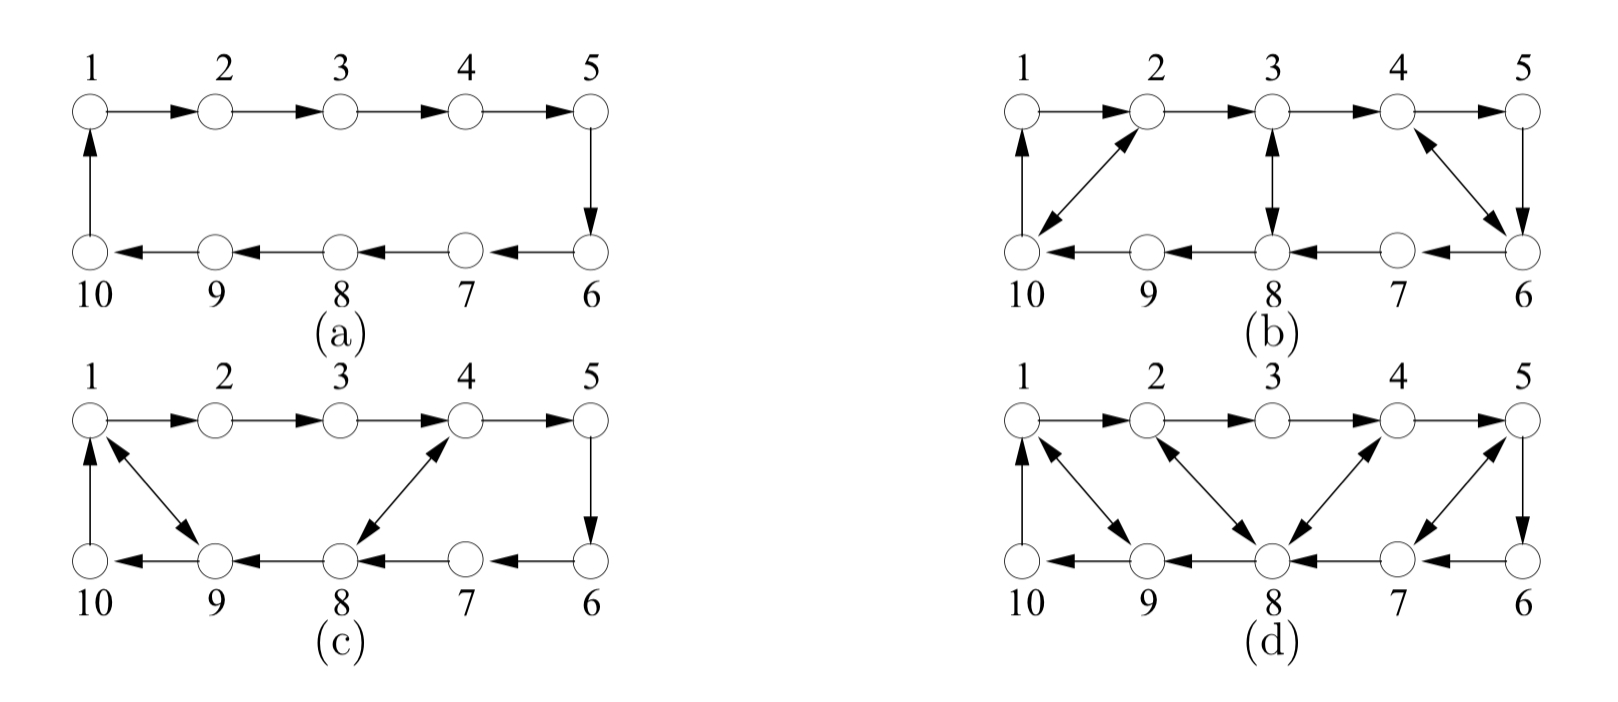
\includegraphics[width=12cm]{figures/Fig4-BalancedSC.jpeg}
    \label{Fig4}
    \caption{For examples of balanced and strongly connected digraphs: (a) $G_a$, (b) $G_b$, (c) $G_c$, and (d) $G_d$ satisfying.}
\end{figure}

{\color[gray]{0.5}
\noindent Figure 4 shows four different networks each with $n=10$ nodes that are all strongly connected and balanced. 
The weights associated with all the edges are 1. 
For the following initial node values satisfying $\text{Ave(x(0))} = 0$
}

\noindent 图(4)展示了四个不同的网络,每个都有$n=10$个节点,这些网络都是强连接并且平衡的。
与所有边相关的权重大小都是1。
对于以下的节点初始值都满足$\text{Ave(x(0))} = 0$

\begin{equation}
    x(0) = (−10.2999, 0.2575, −4.4997, 3.6258, 3.0922, 9.0156, 3.5099, −2.6645, 2.4552, −4.4921)^T
    \notag
\end{equation}

{\color[gray]{0.5}
\noindent we have plotted the state trajectories and the disagreement function $||\delta||^2$ associated with these four digraphs in Figure 5. 
It is clear that as the number of the edges of the graph increase, algebraic connectivity (or $\lambda^2$) increases, and the settling time of the trajectory of the node values decreases. 
The case of a directed cycle of length $n = 10$, or $G_a$, has the largest over-shoot. 
In all four cases, an agreement is asymptotically reached and the performance is improved as a function of $\lambda_2(\hat{G}_k)$ for $k\in \{a,b,c,d\}$.
}

\noindent 我们已经在图(5)中绘制出了状态轨迹,和关于这四个图的非一致函数$||\delta||^2$。
可以清楚的知道,随着图中边数量的增加,代数连通度(或$\lambda^2$)增加,节点的轨迹稳定时间减小。
长度为$n=10$的有向环或$G_a$,具有最大的过冲情况。
在四种情况中,一致性都是逐渐达到的,并且性能随着函数$\lambda_2(\hat{G}_k)$在$k\in \{a,b,c,d\}$中变换而改善。

\begin{figure}[htbp]
    \centering
    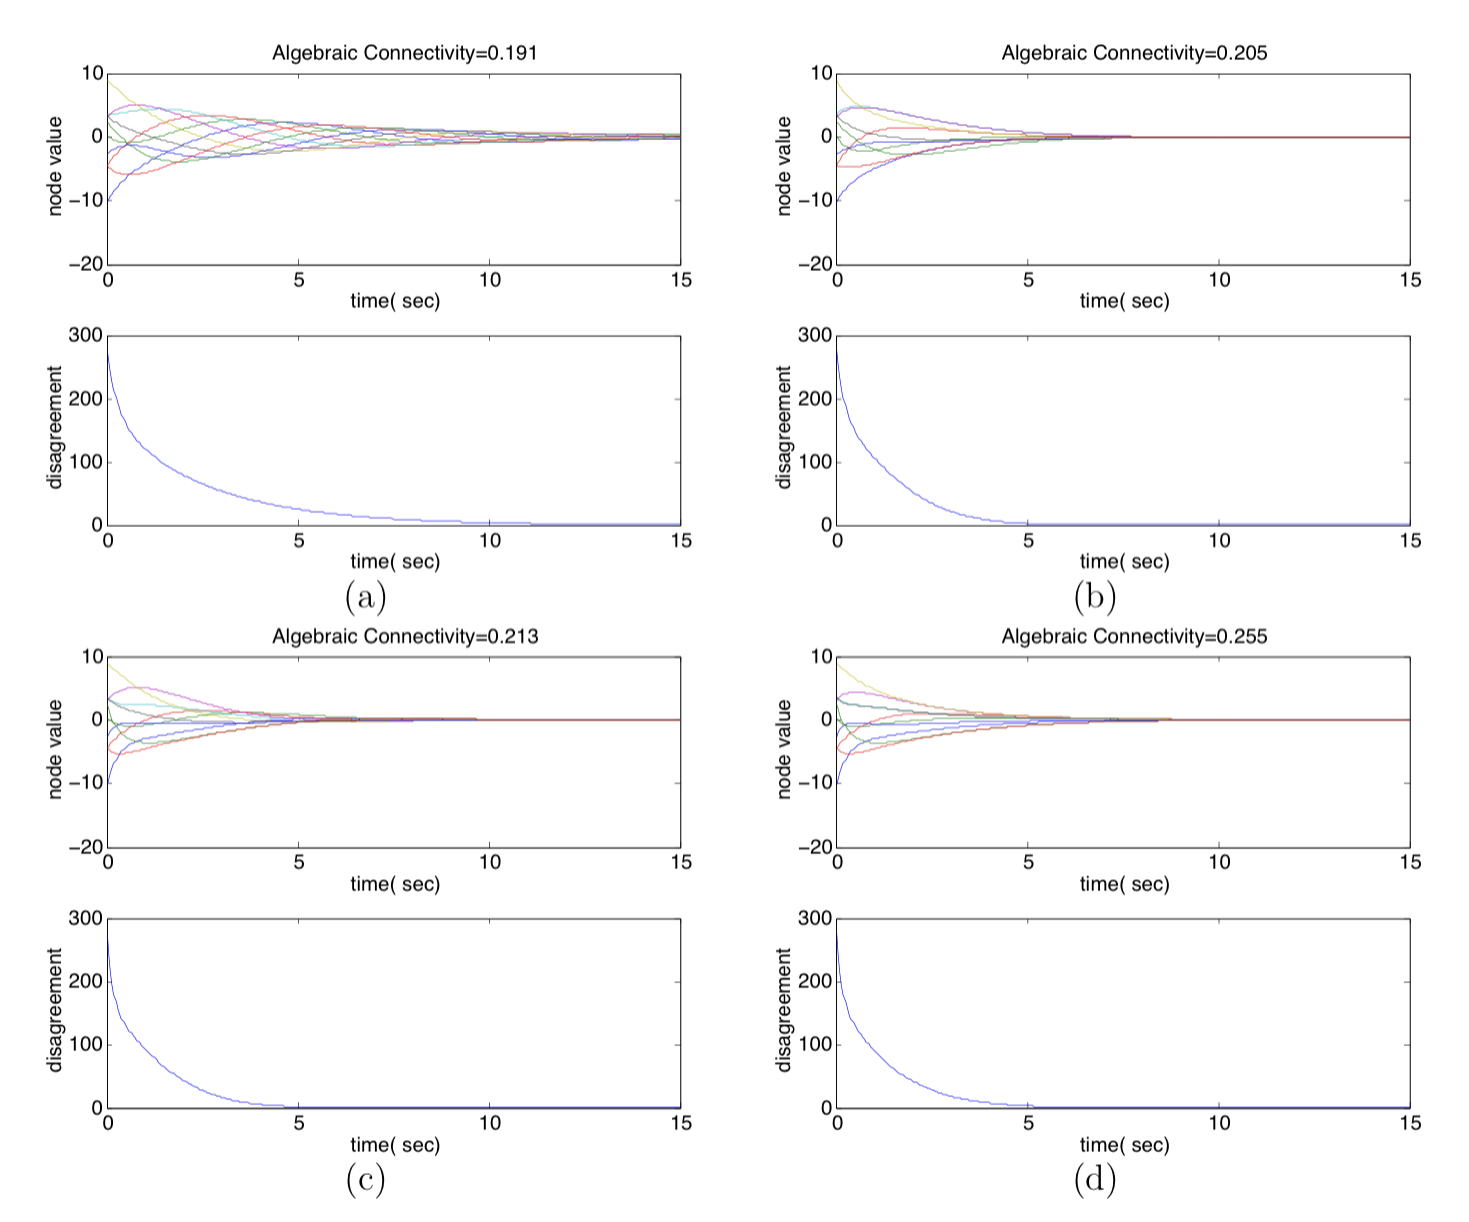
\includegraphics[width=14.5cm]{figures/Fig5-Simulation.jpeg}
    \label{Simulation}
    \caption{For examples of balanced and strongly connected digraphs: (a) $G_a$, (b) $G_b$, (c) $G_c$, and (d) $G_d$ satisfying.}
\end{figure}

{\color[gray]{0.5}
In Figure 6(a), a finite automaton is shown with the set of states \{$G_a, G_b, G_c, G_d$\} representing the discrete-states of a network with switching topology as a hybrid system. 
The hybrid system starts at the discrete-state $G_b$ band switches every $T=1$ second to the next state according to the state machine in Figure 6(a). 
The continuous-time state trajectories and the group disagreement (i.e. $||\delta||^2$) of the network are shown in Figure 6(b). 
Clearly, the group disagreement is monotonically decreasing. 
One can observe that an average-consensus is reached asymptotically. 
Moreover, the group disagreement vanishes exponentially fast.
}

在图6(a)中,一个有限自动机包含了状态集合\{$G_a, G_b, G_c, G_d$\},表示切换拓扑网络作为一个混合系统的离散状态。
这个混合系统从离散状态$G_b$开始,之后每经过$T=1$秒切换至图6(a)所示的下个状态。
网络的连续时间状态轨迹和群组非一致性(即$||\delta||^2$)如图6(b)所示。
清楚的看到,群组非一致性是单调递减的。
可以看到平均一致性是逐渐达成的。
此外,群组非一致性呈指数级快速消失。

\begin{figure}[htbp]
    \centering
    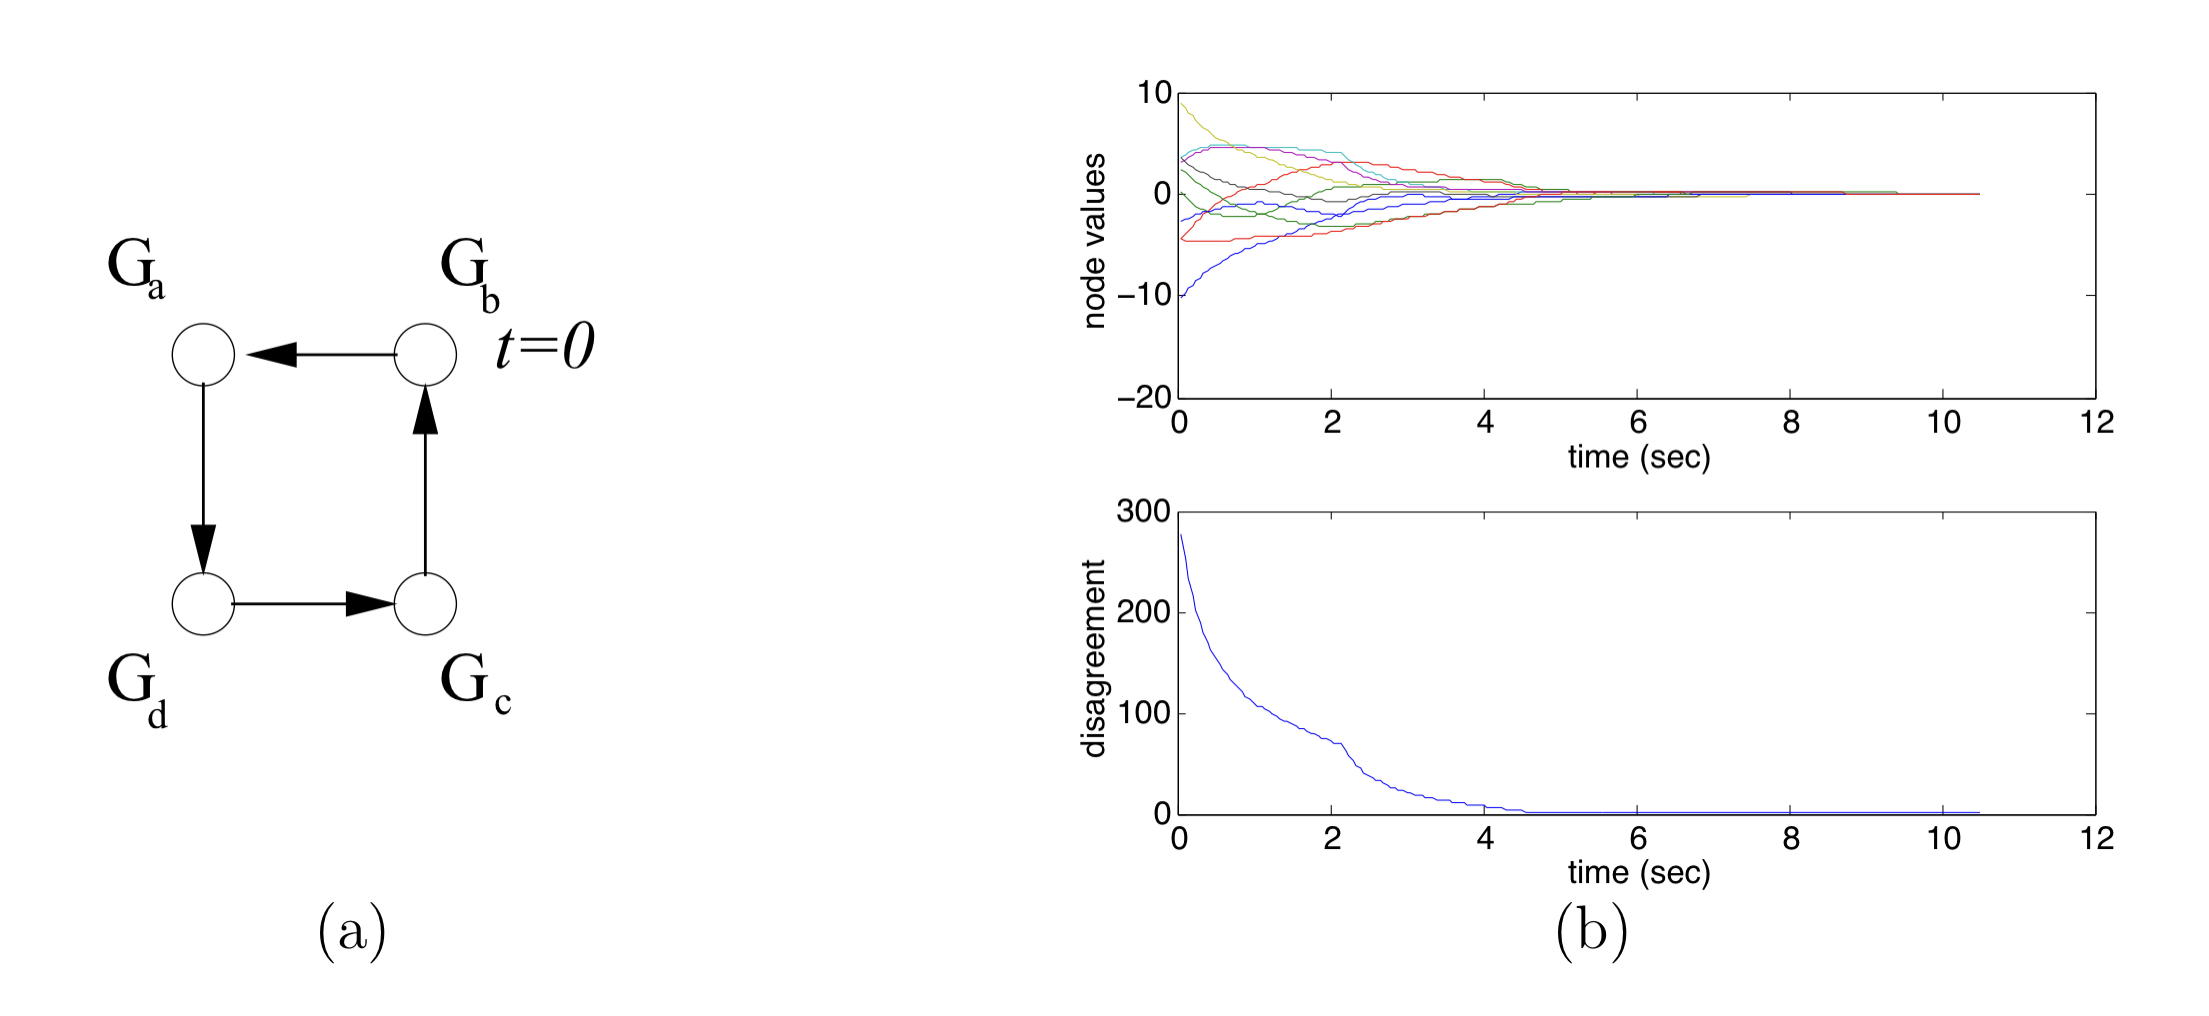
\includegraphics[width=14.5cm]{figures/Fig6-Automaton.jpeg}
    \label{Automaton}
    \caption{(a) A finite automaton with for states representing the discrete-states of a network with variable topology and (b) trajectory of the node values and the group disagreement for a network with a switching information flow.}
\end{figure}

{\color[gray]{0.5}
Next, we present simulation results for average-consensus problem with communication time-delays for a network with information flow shown in Figure 7. 
Figure 8 shows the state trajectories of $n=10$ nodes for a network with communication time-delay $\tau$ for $\tau=0, 0.5\tau_{max}, \tau_{max} = \pi / 2\tau_{max}(G_a) = 0.266$ for a zero-mean random set of initial conditions. 
Clearly, the agreement is achieved for the cases with $\tau < \tau_{max}$ in Figures 8(a), (b), and (c). 
For the case with $\tau = \tau_{max}$, synchronous oscillations are demonstrated in Figure 8(d). 
A third-order Pade approximation is used to model the time-delay as a finite-order LTI system.
}

之后,如图7展示了网络信息流的含通信时滞的平均一致性问题结果。
图8展示了节点$n=10$的含通信时滞网络状态轨迹,沟通时滞$\tau$的值有$\tau=0, 0.5\tau_{max}, \tau_{max} = \pi / 2\tau_{max}(G_a) = 0.266$,做了关于初始条件的0均值随机集合。
清楚的看到,当$\tau < \tau_{max}$时达到一致,如图8(a),(b)和(c)所示。
针对于$\tau = \tau_{max}$的情况,同步振荡如图8(d)所示。
时滞模型使用三阶帕德近似(Pade approximation)作为一个有限阶线性时不变(Linear Time-Invariant, LTI)系统。

\begin{figure}[htbp]
    \centering
    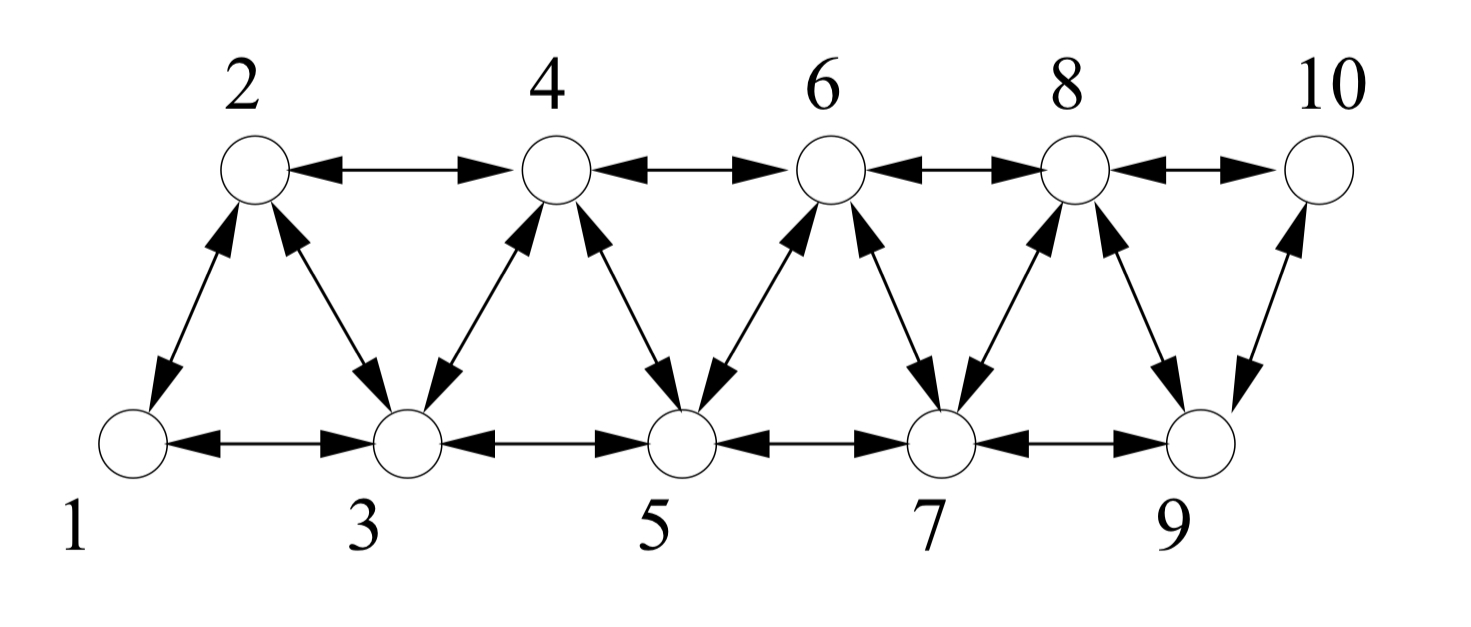
\includegraphics[width=8cm]{figures/Fig7-Undirected.jpeg}
    \label{Undirected}
    \caption{Undirected graph $G_e$ used for consensus with communication time-delays}
\end{figure}

% ------------------------------------------------------------------------------
\section{Conclusions}
{\color[gray]{0.5}
\noindent We provided convergence analysis of consensus protocol for a network of integrators with a directed information flow and fixed or switching topology. 
Our analysis relies on several tools from algebraic graph theory and matrix theory. 
We established a connection between the performance of the linear consensus protocol and the Fiedler eigenvalue of graph Laplacian of the mirror graph. 
A simple disagreement function was introduced as a Lyapunov function for the group disagreement dynamics. 
This was later used to provide a common Lyapunov function that allowed convergence analysis of an agreement protocol for a network with switching topology. 
A commutative diagram was given that shows the operations of taking Laplacian and symmetric part of a matrix commute for weighted adjacency matrices of balanced graphs. 
Balanced graphs turned out to be instrumental in solving average-consensus problems.
}

\noindent 我们展示了了具备有向信息流和固定或切换拓扑积分器网络的一致性协议的收敛性分析。
我们的分析使用了一些代数图论和矩阵论的工具。
我们建立了线性一致性协议的性质和镜像图拉普拉斯矩阵的费德勒特征值之间的联系。
介绍了一个关于群组非一致性变化的李亚普诺夫方程。
这后来作为一个常用的李亚普诺夫函数,用作切换拓扑网络一致性的收敛分析。
给出的交换图展示了将拉普拉斯矩阵和矩阵的渐进部分转变为平衡图的加权邻接矩阵的操作。
平衡图被证明对解决平均一致性问题是有帮助的。

{\color[gray]{0.5}
For networks with undirected graphs, we gave sufficient and necessary conditions for consensus in networks with communication time-delays. 
It was shown that there is a trade-off between robustness to time-delays and the speed of convergence of a linear consensus protocol. 
}

对于无向图网络,我们给出了通信时滞网络一致性的充分必要条件。
这表明在时滞鲁棒性和线性一致性协议收敛速度之间存在折中。

\begin{figure}[htbp]
    \centering
    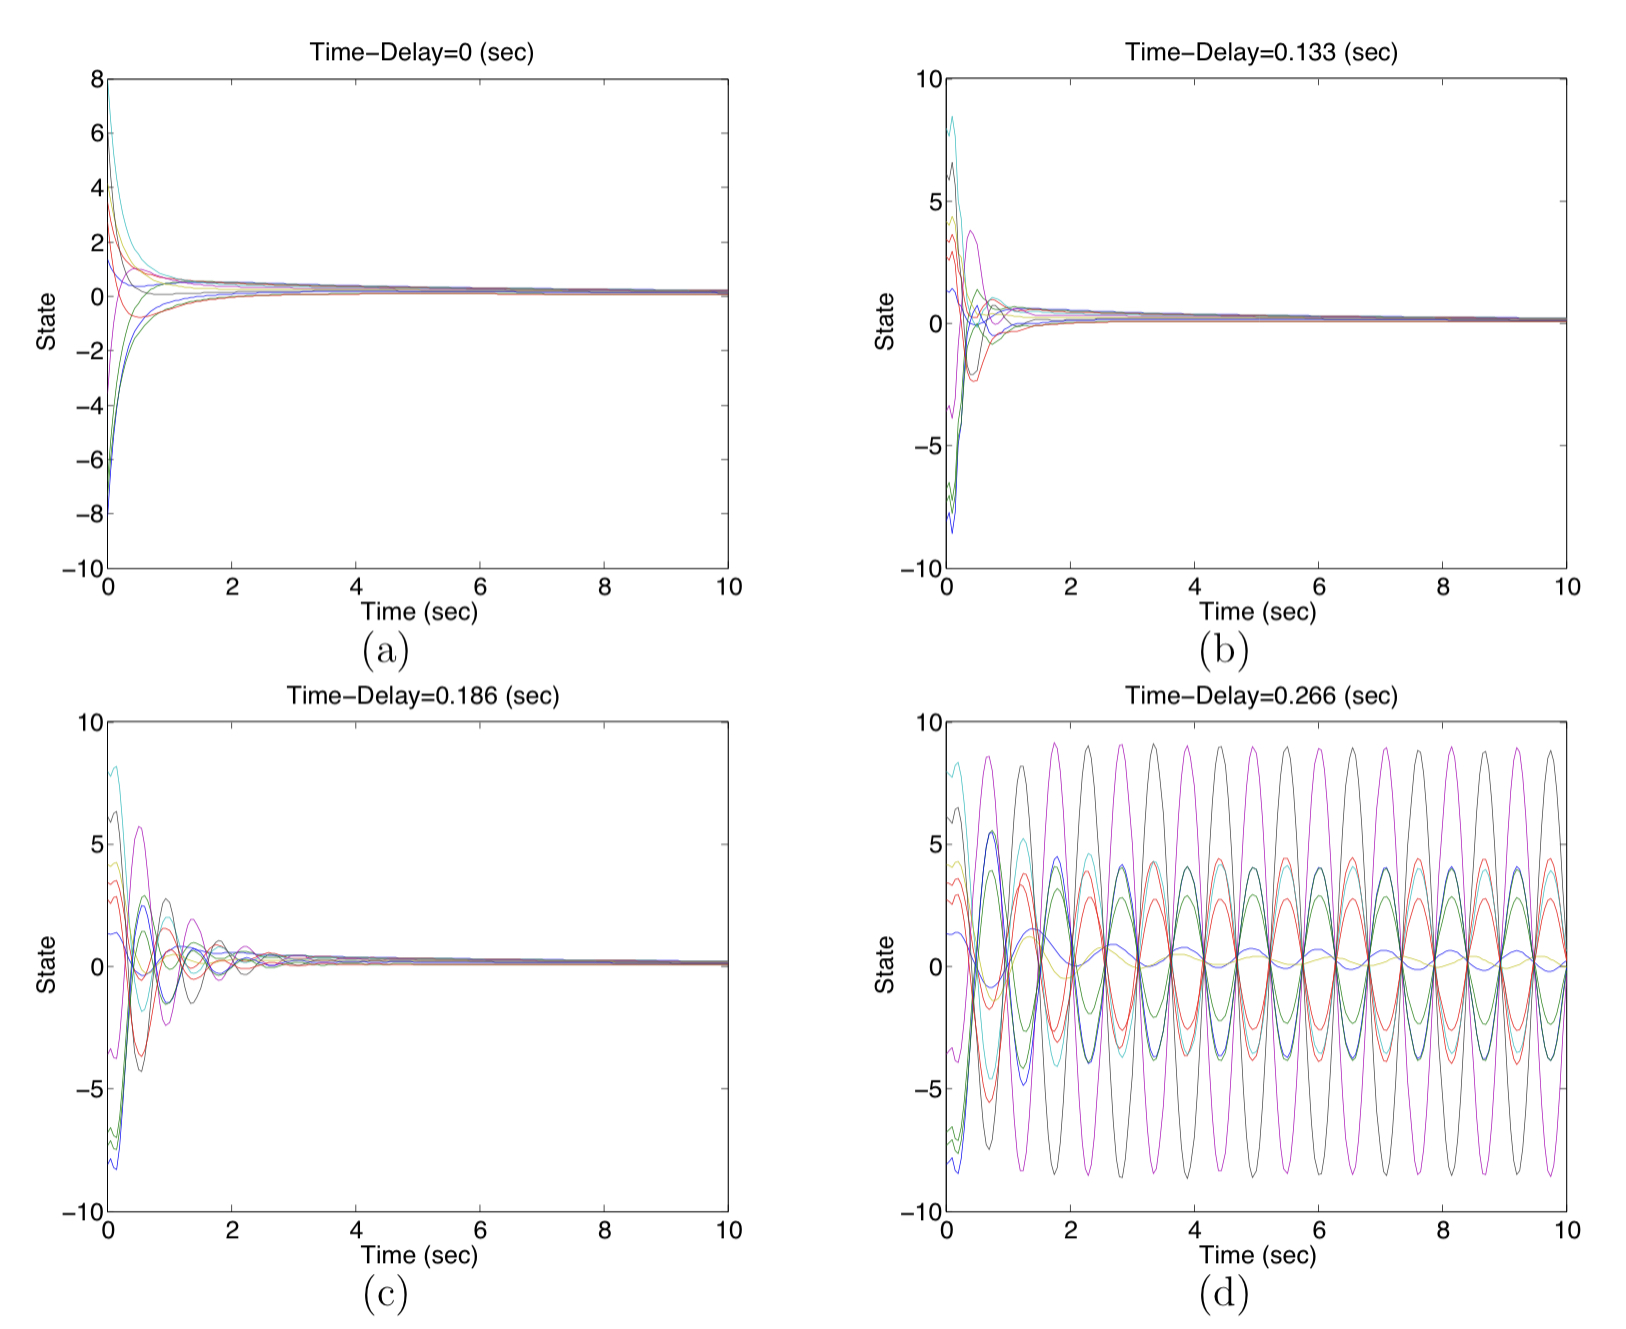
\includegraphics[width=14.5cm]{figures/Fig8-ConsensusProblem.jpeg}
    \label{ConsensusProblem}
    \caption{Consensus problem with communication time-delay on $G_b$ in Figure 7: (a)$\tau$=0, (b)$\tau=0.5\tau_{max}$, (c)$\tau=0.7\tau_{max}$, and (d)$\tau=\tau_{max}$ .}
\end{figure}

{\color[gray]{0.5}
To determine a superior or leader in a group of agents, we introduced max-agents that have a very simple discrete-time model and gave a protocol that solves the max-consensus problem in a distributed way after a maximum of $n−1$ iterations ($n$ is the number of agents).
}

为了确定智能体群组的领导性问题,我们介绍了最大智能体,它拥有一个简单的离散时间模型并且通过最大化的$n-1$次迭代($n$代表智能体的总数),给出了使用分布式方式解决最大一致性问题的协议。

{\color[gray]{0.5}
We presented extensive simulation results that demonstrate the effectiveness of our theoretical results.
}

我们展示了复杂的仿真结果以此演示了我们理论结果的有效性。

{\color[gray]{0.5}
The consensus problems for discrete-time approximation of integrator agents relies on the theory of nonnegative matrices and will be presented in an upcoming paper.
}

积分器智能体的离散时间渐进一致性问题主要依赖非负矩阵理论,这将在下个文章中指出。

% ------------------------------------------------------------------------------
\section*{A Appendix}
{\color[gray]{0.5}
This section contains the proofs of some of the theorems of the paper.
}

这部分包含了文章中一些定理的证明。

\subsection*{A.1 Proof of Theorem 1}
{\color[gray]{0.5}
\noindent \textbf{Proof.} Define $\phi_{ij}(z) = a_{ij}z$ for all $ij \in \mathcal{E}$. 
It is trivial that if $x_i=x_j$ for all $ij \in \mathcal{E}$, then $u=0$. 
Thus, we prove the converse: $u=0$ implies that all nodes are in agreement. 
If the values of all nodes are equal, the result follows. 
Thus, assume there exists a node $i^*$, called max-leader, such that $x_{i^*}\ge x_j$ for all $j\ne i^*$, i.e. $i^* = arg\max_{j\in \mathcal{I}} x_j$ (if $i^*$ is not unique, choose one arbitrarily).
}

\noindent 定义所有的$ij \in \mathcal{E}$有$\phi_{ij}(z) = a_{ij}z$。
不必强调的,对于所有的$ij \in \mathcal{E}$如果有$x_i = x_j$,那么$u=0$。
因此,我们证明收敛性:$u=$表明所有的节点都是一致的。
如果所有节点的值都相等,那么结果正确。
因此,假设存在一个节点$i^*$,称作最大领导者,那么对所有的$j\ne i^*$有$x_{i^*}\ge x_j$,即$i^* = arg\max_{j\in \mathcal{I} x_j}$(即如果$i^*$并不是唯一的,可以任意选择)。

{\color[gray]{0.5}
Define the initial cluster $J^{(0)}=\{ i^* \}$ and denote the indices of all the first-neighbors of $i^*$ by $J^{(1)}=N_{i^*}$. 
Then, $u_{i^*}=0$ implies that
}

定义初始化簇$J^{(0)}=\{ i^* \}$并且用$J^{(1)}=N_{i^*}$来表示所有关于$i^*$的第一邻居序列。
那么,$u_{i^*}=0$意味着

\begin{equation}
    \tag{45}
    \label{45}
    \sum_{j\in N_{i^*}} \phi_{i^*j}(x_j-x_{i^*}) = 0
\end{equation}

{\color[gray]{0.5}
\noindent Since $x_j\le x_{i^*}$ for all $j\in N_{i^*}$ and $\phi_{ij}(z)\le 0$ for $z\le 0$ (i.e. all weights are nonnegative), we get $x_{i^*}=x_j$ for all the first-neighbors $j\in J^{(1)}$, (i.e. the max-leader and all of its first-neighbors are in agreement). 
Next, we define the $k$th-neighbors of $i^*$ and show that the max-leader is in agreement with all of its $k$th-neighbors for $k = 1,\dots, n − 1$. 
The set of $k$th-neighbors of $i^*$ is defined by the following recursive equation
}

\noindent 由于对所有的$j\in N_{i^*}$有$x_j\le x_{i^*}$,对$z\le 0$有$\phi_{ij}(z)\le 0$(即所有的权重都是非负的),我们对所有的第一邻居$j\in J^{(1)}$有$x_{i^*}=x_j$(即最大领导者和所有它的第一邻居是一致的)。
下一步,我们定义$i^*$的第$k$个邻居并证明当最大领导者一致时所有它的$k$个邻居都是一致的,$k = 1,\dots, n − 1$。
关于$i^*$的第$k$个邻居定义为下述递归公式

\begin{equation}
    \tag{46}
    \label{46}
    J^{(k)} = J^{(k-1)} \cup N_{J^{(k-1)}},\quad k\ge 1, J^{(0)}=\{i^*\}
\end{equation}

{\color[gray]{0.5}
\noindent where $N_J$ denotes the set of neighbors of cluster $J\subseteq\mathcal{I}$ (see equation (1)). 
By definition, $\{i^*\}\subset J^{(k)} \subseteq \mathcal{I}$ for $k\ge1$ and $J^{(k)}$ is a monotonically increasing sequence of clusters (in terms of inclusion). 
}

\noindent 这里$N_J$表示簇$J\subseteq\mathcal{I}$的邻居部分。
根据定义,对于$k\ge1$有$\{i^*\}\subset J^{(k)} \subseteq \mathcal{I}$并且$J^{(k)}$是一个关于推论的单调递增序列。

{\color[gray]{0.5}
Notice that in a strongly connected digraph, the maximum length of the minimum path connecting any node $j\ne i^*$ to node $i^*$ is $n-1$. 
Thus, $J^{(n-1)} = \mathcal{I}$. 
By induction, we prove that all the nodes in $J^{(k)}$ are in agreement for $k\ge 1$. 
The statement holds for $k=1$ (i.e. the set of first-neighbors of the max-leader). 
Assume all the nodes in $J^{(k)}$ are in agreement with $i^*$, we show that all the nodes in $J^{(k+1)}$ are in agreement with $i^*$ as well. 
It is sufficient to show this for an arbitrary node $i\in J^{(k)}$ with $N_i \cap (J^{(k+1)}\setminus J^{(k)}) \ne \emptyset$. 
Otherwise, because in a strongly connected digraph $N_i \ne \emptyset$ for all $i$, we get $J^{(k+1)}=J^{(k)}$ and the statement holds. 
For node $i$, we have
}

注意在一个强连通图中,任意节点$j\ne i^*$和节点$i^*$的最短连接路径的最大长度为$n-1$。
因此,$J^{(n-1)} = \mathcal{I}$。
通过归纳法,我们证明在$J^{(k)}$中所有节点对于$k\ge 1$是一致的。
状态满足$k=1$(即最大领导者的第一邻居部分)。
假设所有$J^{(k)}$中的节点都是关于$i^*$一致的,我们也证明了所有在$J^{(k+1)}$中的节点也是关于$i^*$一致的。
可以充分证明对于任意状态节点$i\in J^{(k)}$有$N_i \cap (J^{(k+1)}\setminus J^{(k)}) \ne \emptyset$。
否则的话,因为强连通图关于所有$i$都有$N_i \ne \emptyset$,我们有$J^{(k+1)}=J^{(k)}$并且状态满足。
对于节点$i$,我们有

\begin{equation}
    \tag{47}
    \label{47}
    u_i = \sum_{j\in N_i} \phi_{ij}(x_j-x_i)=0
\end{equation}

{\color[gray]{0.5}
\noindent But $N_i=(N_i\cap J^{(k)})\cup(N_i\cap(\mathcal{I}\setminus J^{(k)}))$ and $\mathcal{I}\setminus J^{(k)}=\mathcal{I}\setminus J^{(k+1)}\cup (J^{(k+1)}\setminus J^{(k)})$. 
Keeping in mind that $J^{(k)}\subset equ\mathcal{I}$ for all $k$ and $J^{(k+1)}$ contains the set of first neighbors of node $i$, i.e. $N_i\subseteq J^{(k+1)}$, we have
}

\noindent 但是$N_i=(N_i\cap J^{(k)})\cup(N_i\cap(\mathcal{I}\setminus J^{(k)}))$ 且 $\mathcal{I}\setminus J^{(k)}=\mathcal{I}\setminus J^{(k+1)}\cup (J^{(k+1)}\setminus J^{(k)})$。
谨记对所有$k$有$J^{(k)}\subset equ\mathcal{I}$且$J^{(k+1)}$包含了节点$i$的第一邻居部分,即$N_i\subseteq J^{(k+1)}$,我们有

\begin{equation}
    \tag{48}
    \label{48}
    N_i \cap (\mathcal{I}\setminus J^{(k)}) = N_i \cap (J^{(k+1)}\setminus J^{(k)})
\end{equation}

{\color[gray]{0.5}
\noindent and
}

\noindent 和

\begin{equation}
    \tag{49}
    \label{49}
    u_i = \sum_{j\in N_i \cap J^{(k)}} \phi_{ij}(x_j-x_i) + \sum_{j\in N_i \cap (J^{(k+1)}\setminus J^{(k)})} \phi_{ij}(x_j-x_i) = 0
\end{equation}

{\color[gray]{0.5}
\noindent The first sum is equal to zero because $x_j=x_i$ all nodes $j\in N_i \cap J^{(k)} \subseteq J^{(k)}$. 
Thus, the second sum must be zero. 
But $x_{i^*}=x_i\ge x_j$ for all $i\in J^{(k)}$ and $j\in \mathcal{I}\setminus J^{(k)}$ which implies all nodes in $N_i \cap (J^{(k+1)}\setminus J^{(k)})$ are in agreement with $i^*$. 
This means that all nodes in the cluster
}

\noindent 因为所有$j\in N_i \cap J^{(k)} \subseteq J^{(k)}$的节点$x_j=x_i$,所以第一求和为0。
因此,第二求和必须也为0。
但是对于所有的$i\in J^{(k)}$和$j\in \mathcal{I}\setminus J^{(k)}$有$x_{i^*}=x_i\ge x_j$,这表明所有在$N_i \cap (J^{(k+1)}\setminus J^{(k)})$中的节点关于$i^*$一致。
这意味着所有簇中的节点

\begin{equation}
    \tag{50}
    \label{50}
\begin{aligned}
    \cup_{i\in J^{(k)}} N_i \cap (J^{(k+1)} \setminus J^{(k)}) &= (\cup_{i\in J^{(k)}} N_i) \cap (J^{(k+1)} \setminus J^{(k)})\\
    &= J^{(k+1)} \cap (J^{(k+1)} \setminus J^{(k)})\\ 
    &= J^{(k+1)} \setminus J^{(k)}
\end{aligned}
\end{equation}

{\color[gray]{0.5}
\noindent are in agreement with $i^*$, i.e. all the nodes in $J^{(k+1)}$ are in agreement. 
Combining this with the fact that $J^{(n-1)}=\mathcal{I}$ we conclude that all the nodes in $\mathcal{I}$ are in agreement.
}

\noindent 是关于节点$i^*$一致,即所有在$J^{(k+1)}$的节点都一致。
结合$J^{(n-1)}=\mathcal{I}$我们可以推断所有在$\mathcal{I}$中的节点一致。

\subsection*{A.2 Proof of Theorem 10}

{\color[gray]{0.5}
\noindent Notice that despite the existence of a nonzero delay $\tau, \sum_{i=1}^{n} u_i=0$. 
Thus, $\alpha=Ave(x)$ is an invariant quantity. 
Given that the solutions of (37) globally asymptotically converge to a limit $x^*$, due to the invariance of $\alpha$, $x_i^*=Ave(x(0)), \forall i \in \mathcal{I}$ and the average-consensus will be reached. 
To establish the stability of (37), we use a frequency domain analysis. 
We have $X(s) = G_{\tau}(s)x(0)$ where
}

\noindent 注意尽管存在一个非零时滞$\tau, \sum_{i=1}^{n} u_i=0$。
因此,$\alpha=Ave(x)$是一个不变量。
给出以下事实,公式(37)全局渐进收敛到$x^*$,由于$\alpha$的不变性,$x_i^*=Ave(x(0)), \forall i \in \mathcal{I}$,并且一致性是可以达到的。
为了建立(37)的稳定性,我们使用频域分析。
我们有$X(s) = G_{\tau}(s)x(0)$这里

\begin{equation}
    \tag{51}
    \label{51}
    G_{\tau}(s) = (sI_n + e^{-\tau s}L)^{-1}
\end{equation}

{\color[gray]{0.5}
\noindent Define $Z_{\tau}(s) = G_{\tau}^{-1}(s) = (sI_n + e^{-\tau s}L)$. 
We need to find sufficient conditions such that all the zeros of $Z_{\tau}(s)$ are on the open LHP or $s=0$. 
Let $w_k$ be the $k$th normalized eigenvector of $L$ associated with the eigenvalue $\lambda_k$ in an increasing order. 
For a connected graph $G$, $0=\lambda_1 < \lambda_2 \le \dots \le \lambda_n =\lambda_{max}(L)$. 
Clearly, $s=0$ in the direction $w_1$ is a zero of the MIMO transfer function $Z_{\tau}(s)$, because $Z_{\tau}(0)w_1 = Lw_1 = 0$. 
Futhermore, any eigen vector of $Z_{\tau}(s)$ is an eigen vector of $L$ and vice verse. 
Let ($s,w_k$) with $k>1$ be a right MIMO transmission zero of $Z_{\tau}(s)$ at frequency $s$ in the direction $w_k$, i.e. $Z_{\tau}(s)w_k=0$. 
Then, $s\ne0$ satisfies the following equation
}

\noindent 定义$Z_{\tau}(s) = G_{\tau}^{-1}(s) = (sI_n + e^{-\tau s}L)$。
我们需要找到一个充分条件如所有$Z_{\tau}(s)$的0都是在开放LHP或$s=0$。
定义$w_k$是$L$关于特征值$\lambda_k$递增顺序排列的第$k$个标准化特征向量。
对于一个连通图$G$,有$0=\lambda_1 < \lambda_2 \le \dots \le  \lambda_n =\lambda_{max}(L)$。
清楚的,在方向$w_1$中$s=0$是MIMO转移函数$Z_{\tau}(s)$的0值,因为$Z_{\tau}(0)w_1 = Lw_1 = 0$。
进一步说,任何关于$Z_{\tau}(s)$的特征向量都是一个属于$L$的特征向量和代替。
定义($s,w_k$)$k>1$是一个在频域$s$属于方向$w_k$上关于$Z_{\tau}(s)$右MIMO转移0,即$Z_{\tau}(s)w_k=0$。
那么,$s\ne0$满足下述方程

\begin{equation}
    \tag{52}
    \label{52}
    s+e^{-\tau s}\lambda_k = 0
\end{equation}

{\color[gray]{0.5}
\noindent or
}

\noindent 或


\begin{equation}
    \tag{53}
    \label{53}
    \frac{1}{\lambda_k} + \frac{e^{-\tau s}\lambda_k}{s} = 0
\end{equation}

{\color[gray]{0.5}
\noindent where $\lambda_k$ is the $k$th eigenvalue of $L$ corresponding to $w_k$. 
This is due to the fact that
}

\noindent 这里$\lambda_k$是$L$关于$w_k$的第$k$个特征值。
这是因为

\begin{equation}
    \tag{54}
    \label{54}
    Z_{\tau}(s) w_k = sw_k + e^{-\tau s}Lw_k = (s+e^{-\tau s}\lambda_k)w_k = 0
\end{equation}

{\color[gray]{0.5}
\noindent but $w_k\ne 0$, thus $s+e^{-\tau}\lambda_k=0$. 
Equation (53) provides a Nyquist criterion for convergence of protocol (A2). 
If the net encirclement of the Nyquist plot of $\Gamma(s) = e^{-\tau s}/s$ around $-1/\lambda_k$ for $k>1$ is zero, then all the zeros of $Z_\tau(s)$(or poles of $G_{\tau}(s)$) other than $s=0$ are stable.
For the special case where $L$ is symmetric, all the eigenvalues are real and the Nyquist stability criterion reduces to zero net encirclement of the Nyquist plot of $\Gamma(s)$ around $-1/\lambda_n$ (note that $\lambda_n=\lambda_{max}(L))$. 
This is because the plot of $\Gamma(jw)$ in the s-plane remains on the right hand side of $-\tau$. 
Since
}

\noindent 但是$w_k\ne 0$,因此$s+e^{-\tau}\lambda_k=0$。
公式(53)协议(A2)收敛分析的奈奎斯特准则。
如果$\Gamma(s) = e^{-\tau s}/s$在$-1/\lambda_k$其中$k>1$附近的网络包围是0,那么所有属于$Z_\tau(s)$的0值(或$G_{\tau}(s)$的极点)不是$s=0$是稳定的。
关于$L$是对称的特殊情况,所有的特征值都是实数并且奈奎斯特稳定准则减小到0。
这是因为$\Gamma(j\omega)$在s平面的图保持在右平面即$-\tau$。
由于

\begin{equation}
    \tag{55}
    \label{55}
    \Gamma(j\omega) = \frac{e^{-j\omega\tau}}{j\omega} = -\frac{sin(\omega\tau)}{\omega} -j\frac{cos(\omega\tau)}{\omega}
\end{equation}

{\color[gray]{0.5}
\noindent and clearly $Re(\Gamma(j\omega))$ is sinc function satisfying $Re(\Gamma(j\omega)) \ge -\tau$. 
A conservative upper bound on $\tau$ can be obtained according to the property $Re(\Gamma(j\omega)) \ge -\tau$ of the Nyquist plot of $\Gamma(s)$ by setting $-1/\lambda_n > -\tau$ which gives the convergence condition $\tau < 1/\lambda_n$. 
As a by-product, for $\tau=0$, the protocol always converges regardless of the value of $\lambda_k, k>1$. 
}

\noindent 并且$Re(\Gamma(j\omega))$是一个满足$Re(\Gamma(j\omega)) \ge -\tau$的sinc函数。
一个在$\tau$上的保守上界。

{\color[gray]{0.5}
A better upper bound on the time-delay $\tau$ can be calculated as follows. 
Let us find the smallest value of the time-delay $\tau>0$ such that $Z_{\tau}(s)$ has a zero on the imaginary axis. 
To do so, set $s=j\omega$ in (52), we have
}



\begin{equation}
    \tag{56}
    \label{56}
    \begin{aligned}
        j\omega + e^{-j\omega\tau} \lambda_k = 0,\\
        -j\omega + e^{j\omega\tau} \lambda_k = 0,
    \end{aligned}
\end{equation}

{\color[gray]{0.5}
\noindent multiplying both sides of the last two equations gives
}



\begin{equation}
    \tag{57}
    \label{57}
    \omega^2 + \lambda_k^2 + j\omega\lambda_k(e^{j\omega\tau}-e^{-j\omega\tau})=0,
\end{equation}

{\color[gray]{0.5}
\noindent or
}



\begin{equation}
    \tag{58}
    \label{58}
    \omega^2 + \lambda_k^2 - 2\omega\lambda_k sin(\omega\tau)=0.
\end{equation}

{\color[gray]{0.5}
\noindent Assuming $\omega>0$ (due to $s\ne 0$), from (58), we get
}



\begin{equation}
    \tag{59}
    \label{59}
    (\omega-\lambda_k)^2 + 2\omega\lambda_k(1-sin(\omega\tau)) = 0.
\end{equation}

{\color[gray]{0.5}
\noindent Since both terms in the left hand side of the last equation are positive semi-definite, the equality holds if and only if both terms are zero, i.e.
}

\begin{equation}
    \tag{60}
    \label{60}
    \begin{aligned}
        \omega = \lambda_k,\\
        sim(\omega\tau) = 1,
    \end{aligned}
\end{equation}

{\color[gray]{0.5}
\noindent This implies $\tau\lambda_k = 2l\pi + \pi/2$ for $l=0,1,2,\dots$, thus the smallest $\tau>0$ satisfies $\tau\lambda_k=\pi/2$. 
Therefore, we have
}



\begin{equation}
    \tag{61}
    \label{61}
    \tau^* = \min_{\substack{\tau\lambda_k=\pi/2\\k>1}}\{\tau\} = \min_{k>1}\frac{\pi}{2\lambda_k}=\frac{\pi}{2\lambda_n}
\end{equation}

{\color[gray]{0.5}
\noindent Due to the continuous dependence of the roots of equation (52) in $\tau$ and the fact that all the zeros of this equation other than $s=0$ for $\tau=0$ are located on the open LHP, for all $\tau\in(0, \tau^*)$, the roots of (52) with $k>1$ are on the open LHP and therefore the poles of $G_{\tau}(s)$ (except for $s=0$) are all stable. 
One can repeat a similar argument for the assumption that $\omega<0$ and get the equation
}



\begin{equation}
    \tag{62}
    \label{62}
    (\omega+\lambda_k)^2 - 2\omega\lambda_k(1+sin(\omega\tau))=0,
\end{equation}

{\color[gray]{0.5}
\noindent which leads to $\omega=-\lambda_k$ and $\tau\lambda_k = 2l\pi + \pi/2$. 
}



{\color[gray]{0.5}
For $\tau=\tau^*$, $G_{\tau}(s)$ has three poles on the imaginary axis given by 
}



\begin{equation}
    \tag{63}
    \label{63}
    s = 0, s \pm j\lambda_n
\end{equation}

{\color[gray]{0.5}
\noindent All other poles of $G_{\tau}(s)$ are stable and in the steady-state the values of each node takes the following form: 
}



\begin{equation}
    \tag{64}
    \label{64}
    x_i^{ss}(t) = a_i + b_i sin(\lambda_nt + \varphi_i),\quad i\in\mathcal{I}
\end{equation}

{\color[gray]{0.5}
\noindent where $a_i,b_i,\varphi_i$ are constants that depend on the initial conditions. 
}



\section*{References}
\noindent [1] N. Biggs. Algebraic Graph Theory. Cambridge Tracks in Mathematics. Cambridge University Press, 1974.

\noindent [2] I. Daubechies and J. C. Lagarias. Sets of matrices all infinite products of which converge. Linear Algebra and Its Applications, 161:227–263, 1992. 

\noindent [3] I. Daubechies and J. C. Lagarias. Corrigendum/addendum to: Sets of matrices all infinite products of which converge. Linear Algebra and Its Applications, 327:69–83, 2001. 

\noindent [4] J. P. Desai, J. P. Ostrowski, and V. Kumar. Modeling and control of formations of nonholonomic mobile robots. IEEE Trans. on Robotics and Automation, 17(6), December 2002. 

\noindent [5] R. Diestel. Graph Theory, volume 173 of Graduate Texts in Mathematics. SpringerVerlag, 2000.

\noindent [6] A. Fax and R. M. Murray. Graph Laplacians and stabilization of vehicle formations. The 15th IFAC World Congress, June 2002. 

\noindent [7] A. Fax and R. M. Murray. Information Flow and Cooperative Control of Vehicle Formations. The 15th IFAC World Congress, June 2002. 

\noindent [8] M. Fiedler. Algebraic connectivity of graphs. Czechoslovak Mathematical Journal, 23(98):298–305, 1973.

\noindent [9] M. Fiedler. A property of eigenvectors of nonnegative symmetric matrices and its application to graph theory. Czechoslovak Mathematical Journal, 25(100):619–633, 1975. 

\noindent [10] F. R. Gantmacher. Matrix Theory, volume II. Chelsea Publishing Company, 1959. 

\noindent [11] C. Godsil and G. Royle. Algebraic Graph Theory, volume 207 of Graduate Texts in Mathematics. Springer, 2001. 

\noindent [12] R. A. Horn and C. R. Johnson. Matrix Analysis. Cambridge University Press, 1987. 

\noindent [13] A. Jadbabaie, J. Lin, and S. A. Morse. Coordination of groups of mobile agents using nearest neighbor rules. IEEE Trans. on Automatic Control (to appear). 

\noindent [14] R. W. Lawton, J. R. T. Beard and B. J. Young. A Decentralized Approach to Formation Maneuvers. IEEE Trans. on Robotics and Automation (to appear). 

\noindent [15] N. A. Lynch. Distributed Algorithms. Morgan Kaufmann Publishers, Inc., 1997. 

\noindent [16] M. Marcus and H. Minc. A Survey of Matrix Theory and Matrix Inequalities. Dover Publications, 1969. 

\noindent [17] R. Merris. Laplacian matrices of a graph: a survey. Linear Algebra and its Applications, 197:143–176, 1994. 

\noindent [18] M. Mesbahi. On a dynamic extension of the theory of graphs. Proc. of the American Control Conference, Anchorange, AL, May 2002. 

\noindent [19] M. Mesbahi and F. Y. Hadegh. Formation flying of multiple spacecraft via graphs, matrix inequalities, and switching. AIAA Journal of Guidance, Control, and Dynamics, 24(2):369–377, March 2000. 

\noindent [20] R. Olfati Saber and R. M. Murray. Consensus Protocols for Networks of Dynamic Agents. Proc. of the American Control Conference, June 2003. 

\noindent [21] F. Paganini, J. Doyle, and S Low. Scalable laws for stable network congestion control. Proc. of the Int. Conf. on Decision and Control, Orlando, FL, Dec. 2001. 

\noindent [22] C. W. Reynolds. Flocks, herds, and schools: a distributed behavioral model. Computer Graphics (ACM SIGGRAPH ’87 Conference Proceedings), 21(4):25–34, July 1987. 

\noindent [23] J. Toner and Y. Tu. Flocks, herds, and schools: A quantitative theory of flocking. Physical Review E, 58(4):4828–4858, October 1998. 

\noindent [24] T. Vicsek, A. Cziro´ok, E. Ben-Jacob, and O. Cohen, I. Shochet. Novel type of phase transition in a system of self-deriven particles. Physical Review Letters, 75(6):1226–1229, August, 1995.

\noindent [25] H. Yamaguchi, T. Arai, and G. Beni. A distributed control scheme for multiple robotic vehicles to make group formations. Robotics and Autonomous Systems, 36:125–147, 2001


\section*{Figures and Codes}

\begin{figure}[htbp]
    \centering
    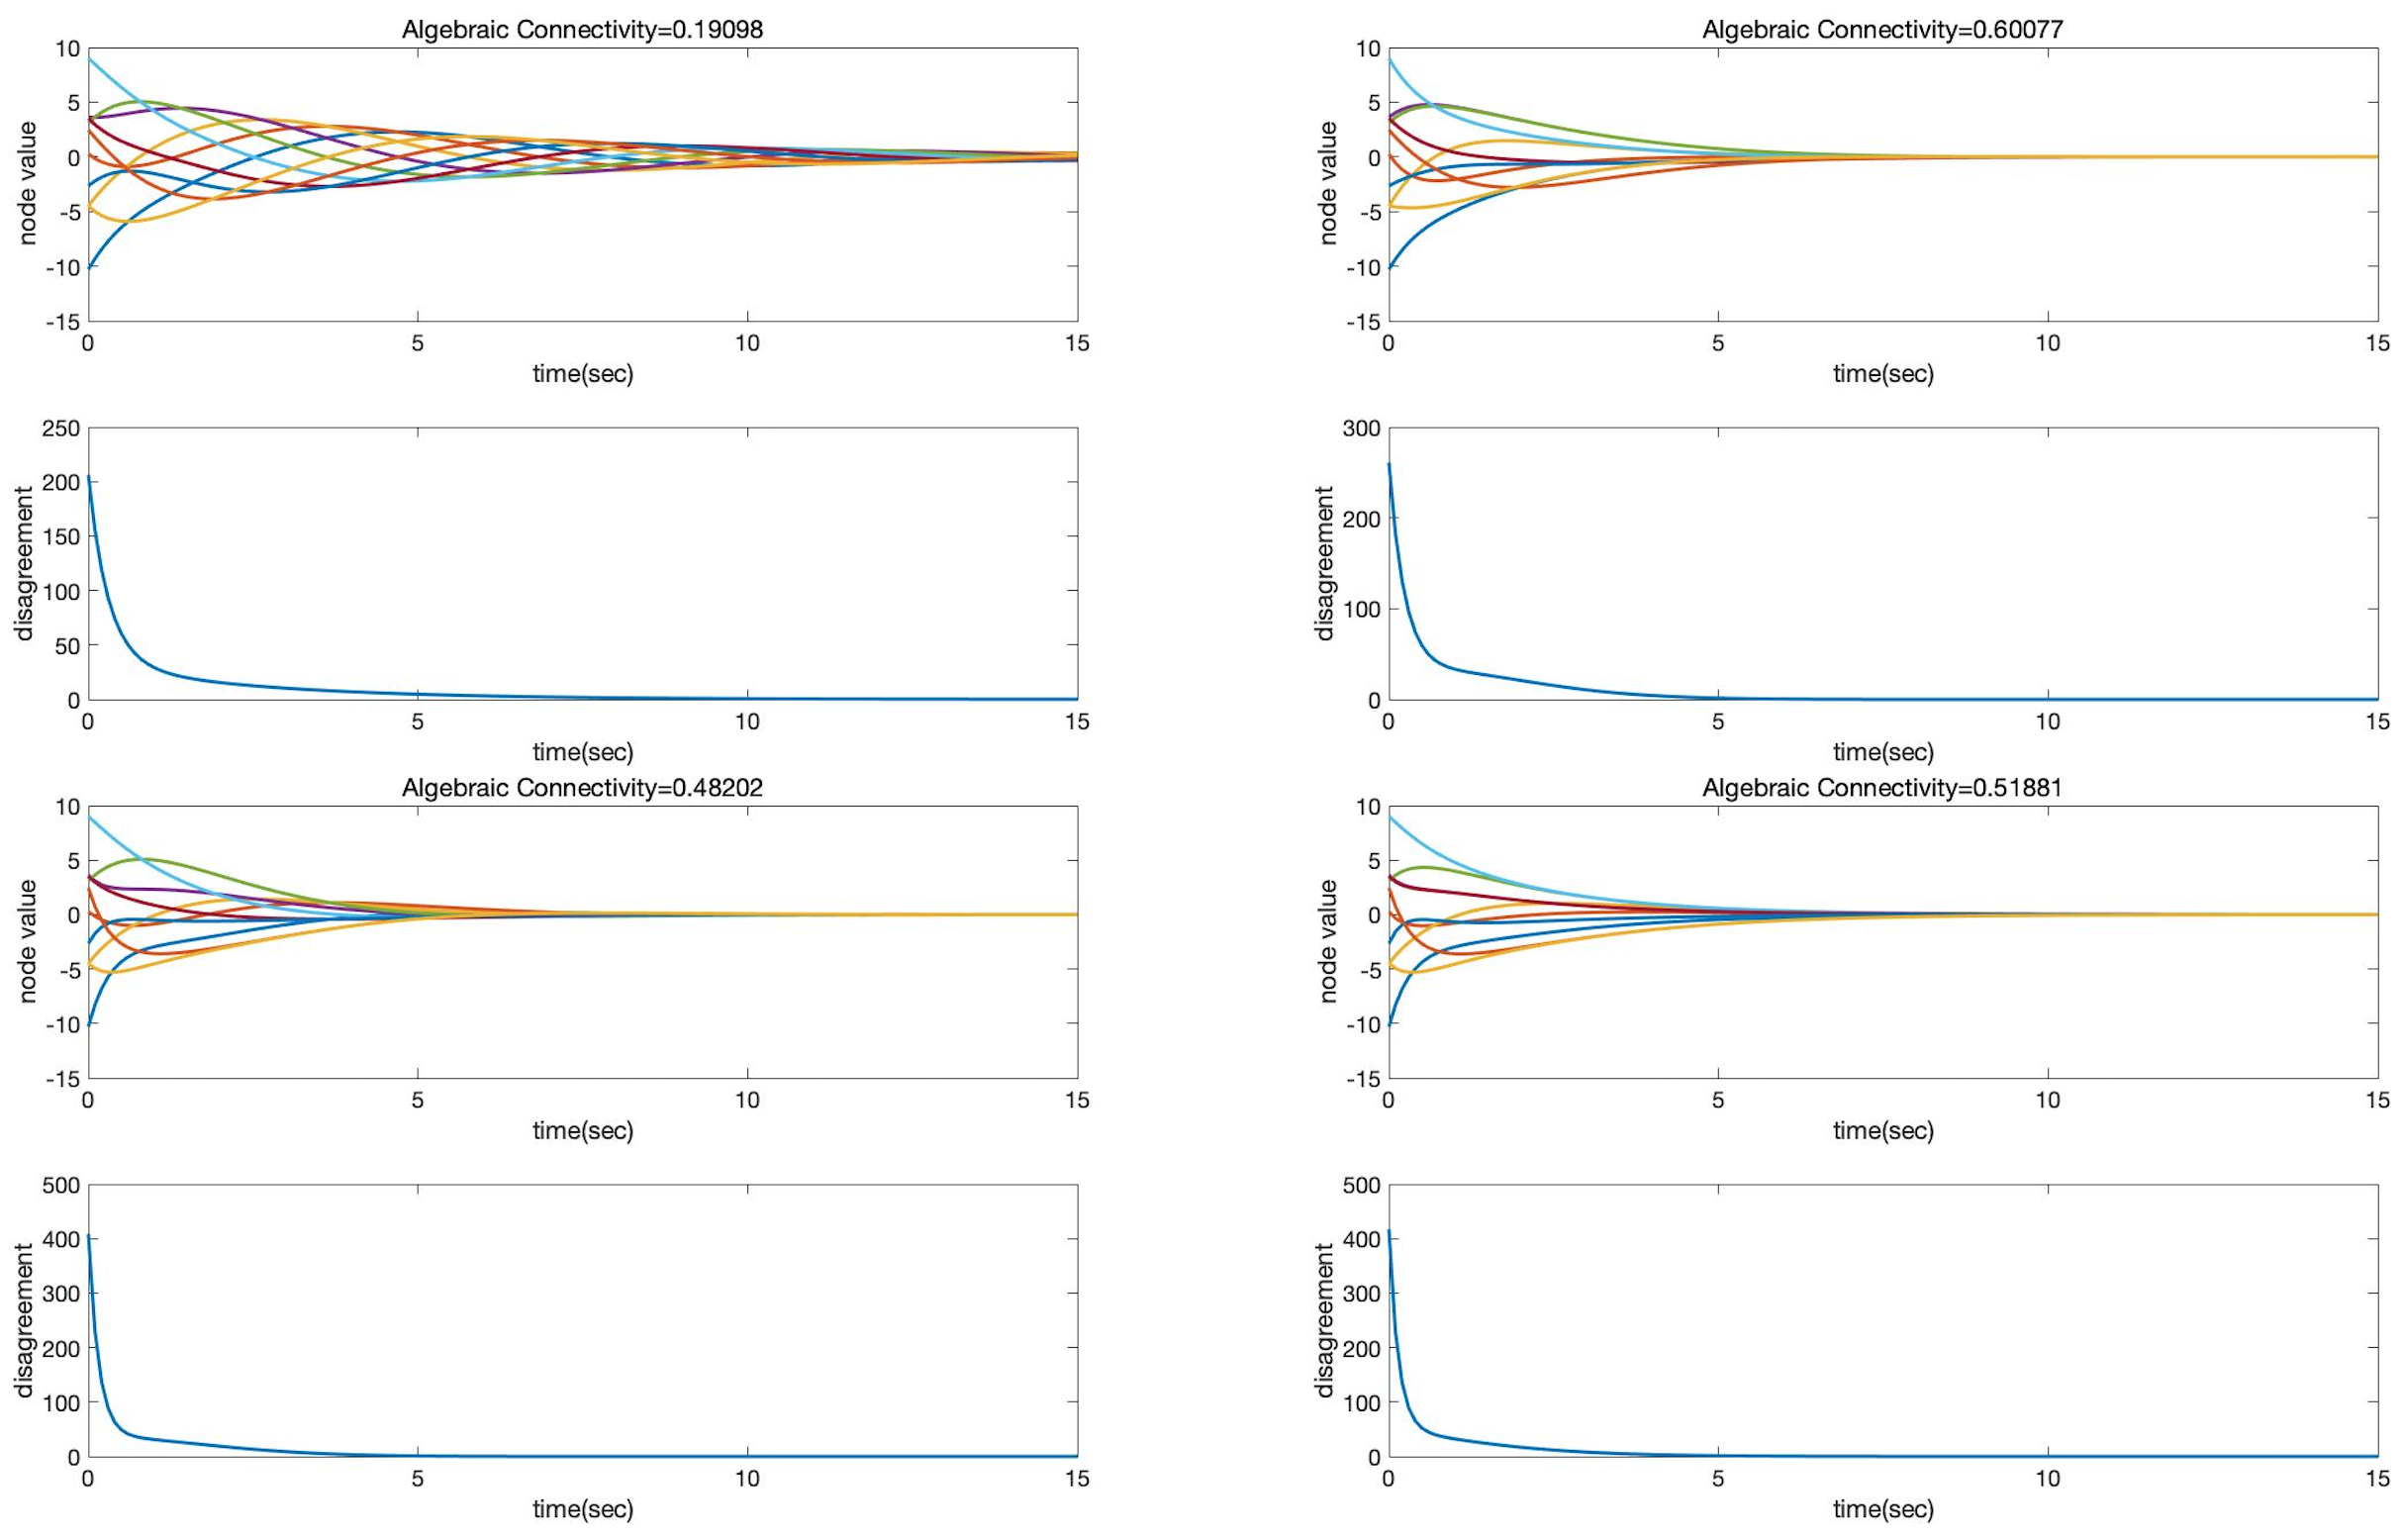
\includegraphics[width=14.5cm]{figures/UserFig5.png}
    \caption{Result for Figure5 of Paper}
    \label{UserFig5}
\end{figure}

\begin{figure}[htbp]
    \centering
    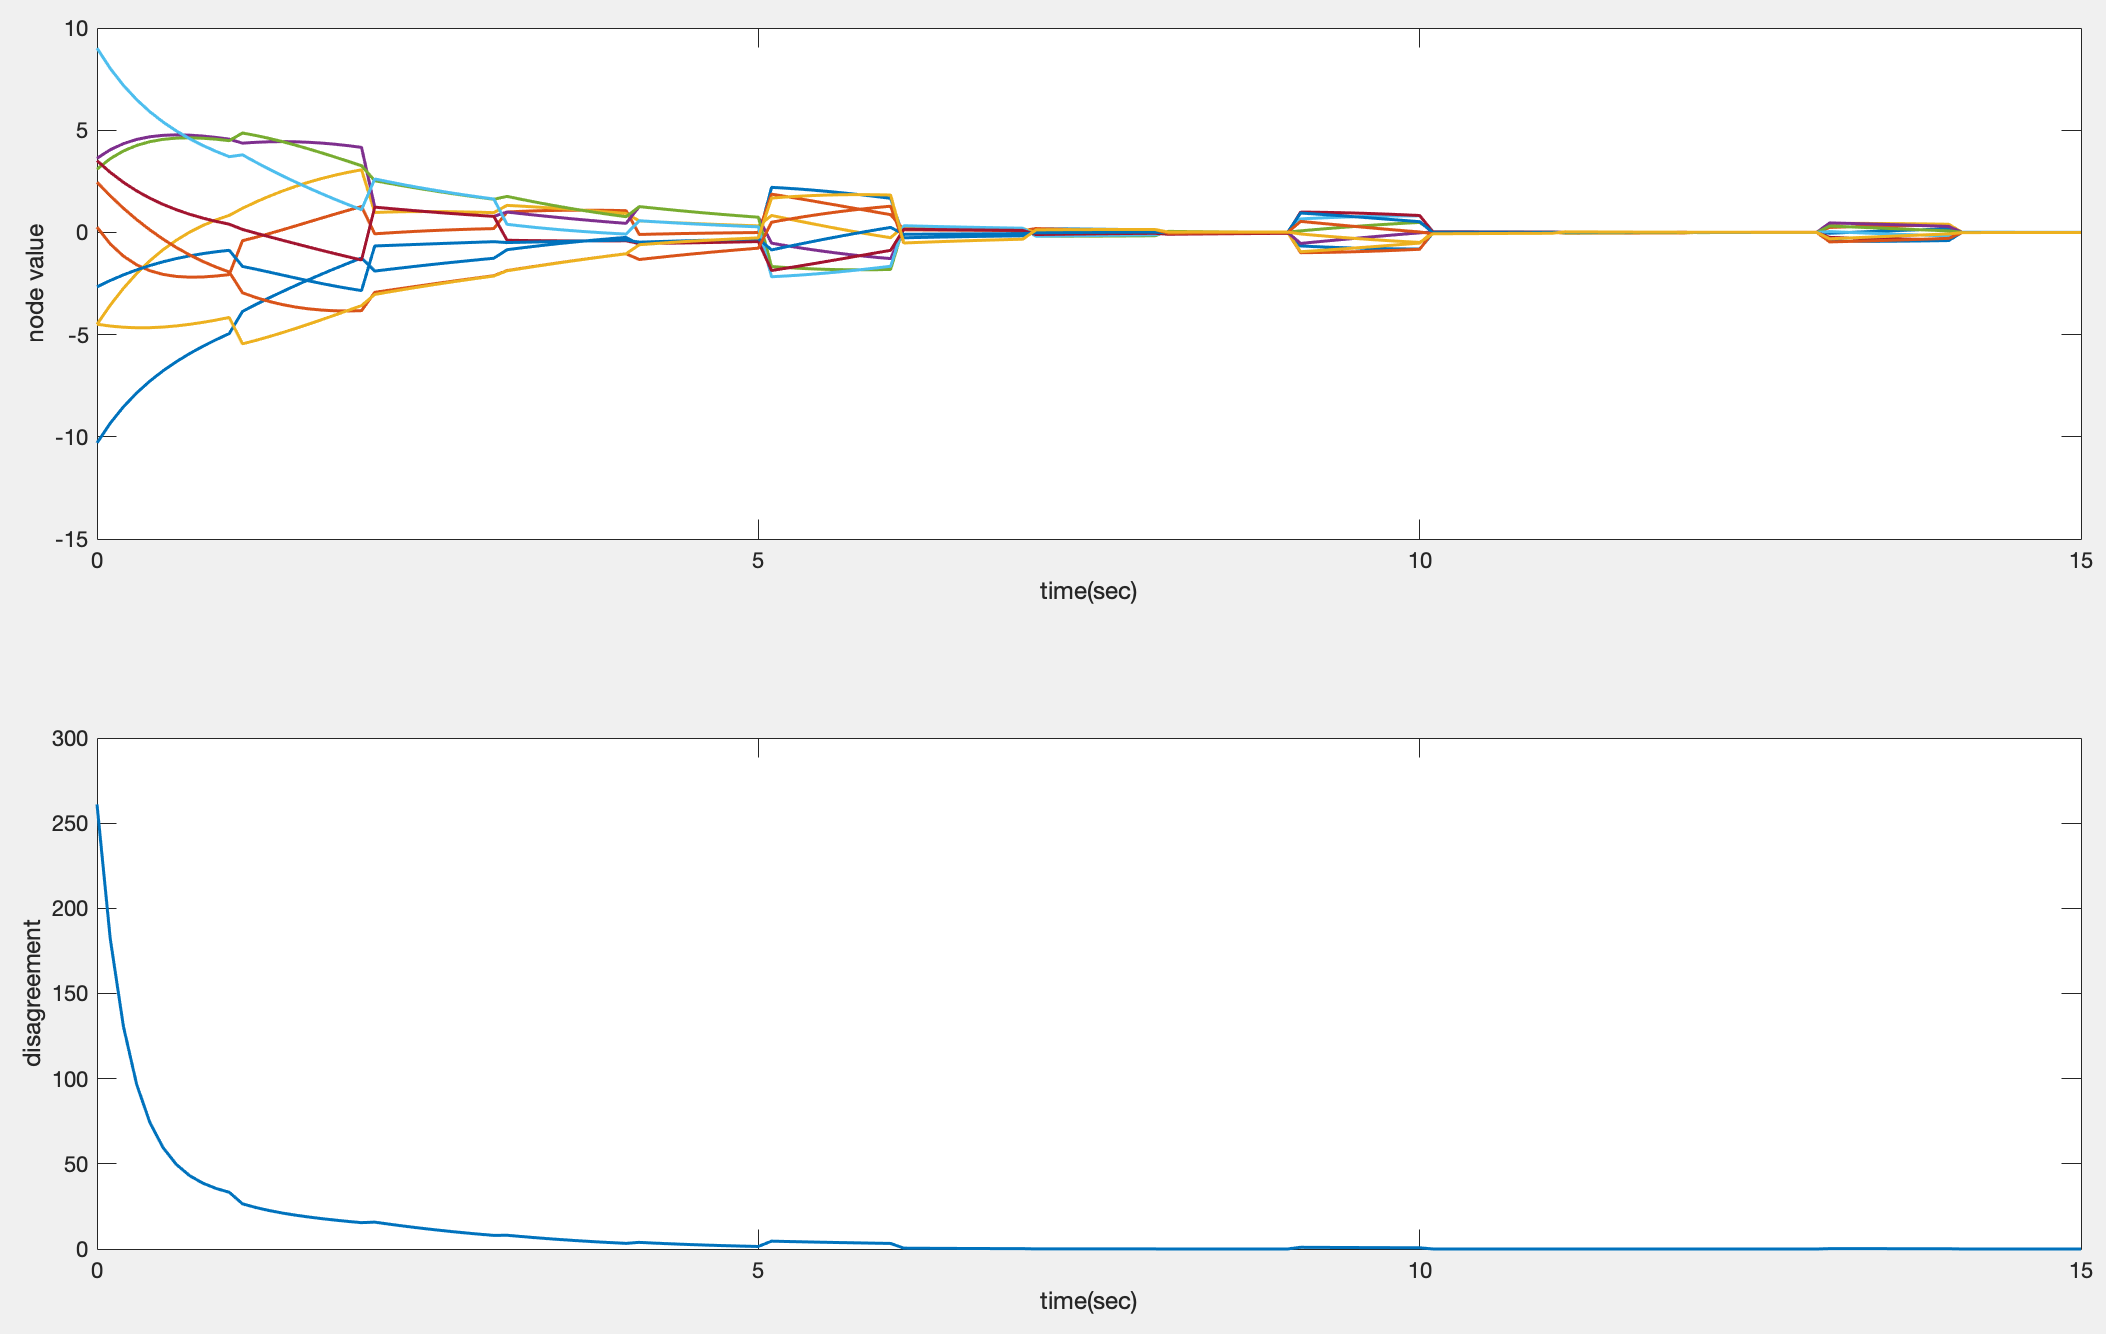
\includegraphics[width=14.5cm]{figures/UserFig6.png}
    \caption{Result for Figure6 of Paper}
    \label{UserFig5}
\end{figure}

\begin{figure}[htbp]
    \centering
    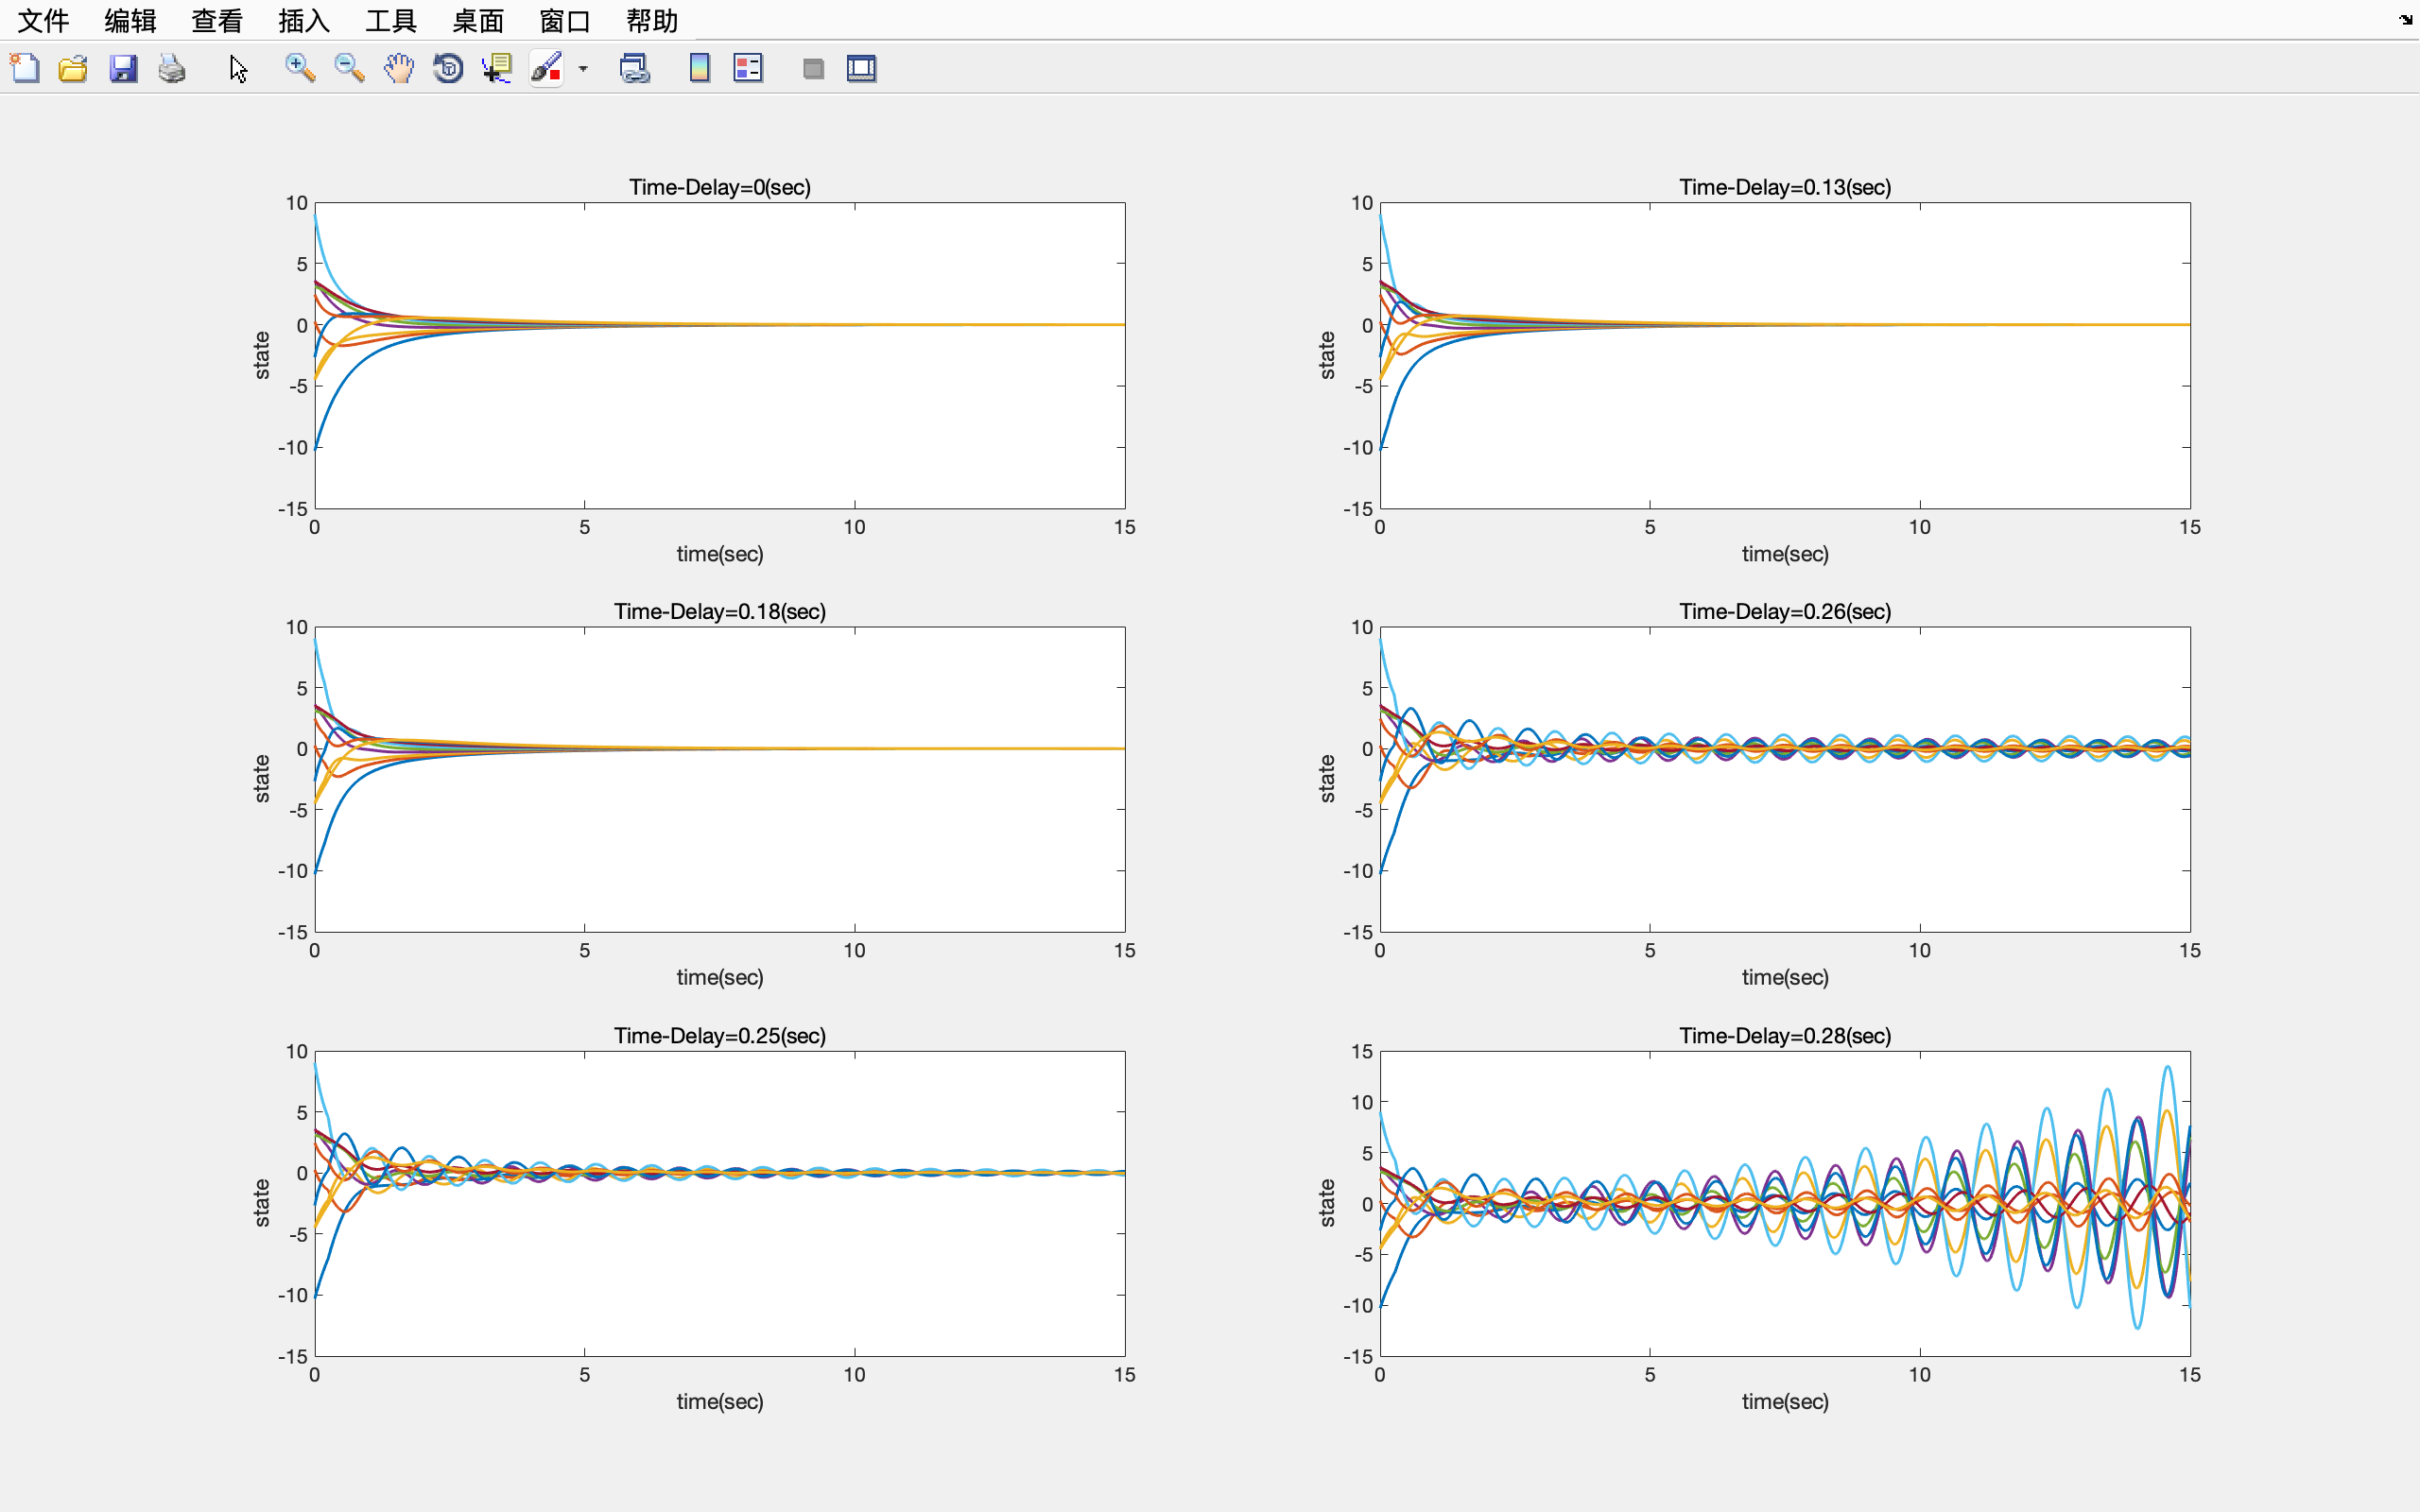
\includegraphics[width=14.5cm]{figures/UserFig83.png}
    \caption{Result for Figure8 of Paper}
    \label{UserFig5}
\end{figure}

\subsection*{Codes for Figure5 of Paper}
\begin{lstlisting}
clear;
clc;
% 此为原Paper中第六部分测试代码

% 状态初值如下
X0  = [-10.2999, 0.2575, -4.4997, 3.6258, 3.0922, 9.0156, 3.5099, -2.6645, 2.4552, -4.4921]';

Node_Nums = 10;

% b图度矩阵,邻接矩阵,拉普拉斯矩阵
D_a = [ 1 0 0 0 0 0 0 0 0 0;
        0 1 0 0 0 0 0 0 0 0;
        0 0 1 0 0 0 0 0 0 0;
        0 0 0 1 0 0 0 0 0 0;
        0 0 0 0 1 0 0 0 0 0;
        0 0 0 0 0 1 0 0 0 0;
        0 0 0 0 0 0 1 0 0 0;
        0 0 0 0 0 0 0 1 0 0;
        0 0 0 0 0 0 0 0 1 0;
        0 0 0 0 0 0 0 0 0 1;];
A_a = [ 0 1 0 0 0 0 0 0 0 0;
        0 0 1 0 0 0 0 0 0 0;
        0 0 0 1 0 0 0 0 0 0;
        0 0 0 0 1 0 0 0 0 0;
        0 0 0 0 0 1 0 0 0 0;
        0 0 0 0 0 0 1 0 0 0;
        0 0 0 0 0 0 0 1 0 0;
        0 0 0 0 0 0 0 0 1 0;
        0 0 0 0 0 0 0 0 0 1;
        1 0 0 0 0 0 0 0 0 0;];
L_a = D_a - A_a;

% b图度矩阵,邻接矩阵,拉普拉斯矩阵
D_b = [ 1 0 0 0 0 0 0 0 0 0;
        0 2 0 0 0 0 0 0 0 0;
        0 0 2 0 0 0 0 0 0 0;
        0 0 0 2 0 0 0 0 0 0;
        0 0 0 0 1 0 0 0 0 0;
        0 0 0 0 0 2 0 0 0 0;
        0 0 0 0 0 0 1 0 0 0;
        0 0 0 0 0 0 0 2 0 0;
        0 0 0 0 0 0 0 0 1 0;
        0 0 0 0 0 0 0 0 0 2;];
A_b = [ 0 1 0 0 0 0 0 0 0 0;
        0 0 1 0 0 0 0 0 0 1;
        0 0 0 1 0 0 0 1 0 0;
        0 0 0 0 1 1 0 0 0 0;
        0 0 0 0 0 1 0 0 0 0;
        0 0 0 1 0 0 1 0 0 0;
        0 0 0 0 0 0 0 1 0 0;
        0 0 1 0 0 0 0 0 1 0;
        0 0 0 0 0 0 0 0 0 1;
        1 1 0 0 0 0 0 0 0 0;];
L_b = D_b - A_b;

% c图度矩阵,邻接矩阵,拉普拉斯矩阵
D_c = [ 2 0 0 0 0 0 0 0 0 0;
        0 1 0 0 0 0 0 0 0 0;
        0 0 1 0 0 0 0 0 0 0;
        0 0 0 2 0 0 0 0 0 0;
        0 0 0 0 1 0 0 0 0 0;
        0 0 0 0 0 1 0 0 0 0;
        0 0 0 0 0 0 1 0 0 0;
        0 0 0 0 0 0 0 2 0 0;
        0 0 0 0 0 0 0 0 2 0;
        0 0 0 0 0 0 0 0 0 1;];
A_c = [ 0 1 0 0 0 0 0 0 1 0;
        0 0 1 0 0 0 0 0 0 0;
        0 0 0 1 0 0 0 0 0 0;
        0 0 0 0 1 0 0 1 0 0;
        0 0 0 0 0 1 0 0 0 0;
        0 0 0 0 0 0 1 0 0 0;
        0 0 0 0 0 0 0 1 0 0;
        0 0 0 1 0 0 0 0 1 0;
        1 0 0 0 0 0 0 0 0 1;
        1 0 0 0 0 0 0 0 0 0;];
L_c = D_c - A_c;

% d图度矩阵,邻接矩阵,拉普拉斯矩阵
D_d = [ 2 0 0 0 0 0 0 0 0 0;
        0 2 0 0 0 0 0 0 0 0;
        0 0 1 0 0 0 0 0 0 0;
        0 0 0 2 0 0 0 0 0 0;
        0 0 0 0 2 0 0 0 0 0;
        0 0 0 0 0 1 0 0 0 0;
        0 0 0 0 0 0 2 0 0 0;
        0 0 0 0 0 0 0 3 0 0;
        0 0 0 0 0 0 0 0 2 0;
        0 0 0 0 0 0 0 0 0 1;];
% 邻接矩阵,有向拓扑结构
A_d = [ 0 1 0 0 0 0 0 0 1 0;
        0 0 1 0 0 0 0 1 0 0;
        0 0 0 1 0 0 0 0 0 0;
        0 0 0 0 1 0 0 1 0 0;
        0 0 0 0 0 1 1 0 0 0;
        0 0 0 0 0 0 1 0 0 0;
        0 0 0 0 1 0 0 1 0 0;
        0 1 0 1 0 0 0 0 1 0;
        1 0 0 0 0 0 0 0 0 1;
        1 0 0 0 0 0 0 0 0 0;];
L_d = D_d - A_d;

% 设置收敛相关参数
tBegin = 0;                     % 开始时间 
tEnd   = 15;                    % 结束时间
dt     = 0.1;                   % 最小时间间隔
times  = (tEnd-tBegin) / dt;    % 迭代计算次数
time   = 1;
% 定义记录时间数组
t(:,1)   = tBegin;
% 定义图a数据存储数组
X_a(:,1) = X0;
U_a(:,1) = -L_a * X0;
Delta_a(:,1) = X0' * L_a * X0;
% 定义图b数据存储数组
X_b(:,1) = X0;
U_b(:,1) = -L_b * X0;
Delta_b(:,1) = X0' * L_b * X0;

X_c(:,1) = X0;
U_c(:,1) = -L_c * X0;
Delta_c(:,1) = X0' * L_c * X0;

X_d(:,1) = X0;
U_d(:,1) = -L_d * X0;
Delta_d(:,1) = X0' * L_d * X0;
% 开始收敛计算
while(time <= times)
    t(:,time+1) = tBegin + time * dt;
    % 图a数据迭代
    X_a(:,time+1) = expm(-L_a * t(:,time+1)) * X0;                          % Xt = expm(-Lx)*X0 添加更新后的Xt值
    U_a(:,time+1) = -L_a * X_a(:,time+1);                                   % Ut = -LXt 添加更新后的Ut值 
    Delta_a(:,time+1) = X_a(:,time+1)'*L_a*X_a(:,time+1);                   % Delta = XT * L * X
    % 图b数据迭代
    X_b(:,time+1) = expm(-L_b * t(:,time+1)) * X0;
    U_b(:,time+1) = -L_b * X_b(:,time+1);
    Delta_b(:,time+1) = X_b(:,time+1)'*L_b*X_b(:,time+1);

    X_c(:,time+1) = expm(-L_c * t(:,time+1)) * X0;
    U_c(:,time+1) = -L_c * X_c(:,time+1);
    Delta_c(:,time+1) = X_c(:,time+1)'*L_c*X_c(:,time+1);

    X_d(:,time+1) = expm(-L_d * t(:,time+1)) * X0;
    U_d(:,time+1) = -L_d * X_d(:,time+1);
    Delta_d(:,time+1) = X_d(:,time+1)'*L_d*X_d(:,time+1);

    time = time + 1;
end

% 矩阵的代数连通度
eig_val_a = eig(L_a);                       % L a的特征值
eig_val_a = sort(eig_val_a,'ascend');       % 从小到大排序,最小特征值为0
AC_a      = real(eig_val_a(2));             % algebraic connectivity 代数连通度:lap matrix的第二小特征值>0,连通图

eig_val_b = eig(L_b);                       % L b的特征值
eig_val_b = sort(eig_val_b,'ascend');       % 从小到大排序,最小特征值为0
AC_b      = real(eig_val_b(2));             % algebraic connectivity 代数连通度:lap matrix的第二小特征值>0,连通图

eig_val_c = eig(L_c);
eig_val_c = sort(eig_val_c,'ascend');
AC_c      = real(eig_val_c(2));

eig_val_d = eig(L_d);
eig_val_d = sort(eig_val_d,'ascend');
AC_d      = real(eig_val_d(2));

% 绘制图a数据
subplot(4,2,1);
plot(t,X_a(1,:), t,X_a(2,:), t,X_a(3,:), t,X_a(4,:), t,X_a(5,:), t,X_a(6,:), t,X_a(7,:), t,X_a(8,:), t,X_a(9,:), t,X_a(10,:), 'linewidth',1.0)
xlabel("time(sec)");ylabel("node value");
title("Algebraic Connectivity="+num2str(AC_a));
subplot(4,2,3);
plot(t,Delta_a, 'linewidth',1.0);
xlabel("time(sec)");ylabel("disagreement");

subplot(4,2,2);
plot(t,X_b(1,:), t,X_b(2,:), t,X_b(3,:), t,X_b(4,:), t,X_b(5,:), t,X_b(6,:), t,X_b(7,:), t,X_b(8,:), t,X_b(9,:), t,X_b(10,:), 'linewidth',1.0)
xlabel("time(sec)");ylabel("node value");
title("Algebraic Connectivity="+num2str(AC_b));
subplot(4,2,4);
plot(t,Delta_b, 'linewidth',1.0);
xlabel("time(sec)");ylabel("disagreement");

subplot(4,2,5);
plot(t,X_c(1,:), t,X_c(2,:), t,X_c(3,:), t,X_c(4,:), t,X_c(5,:), t,X_c(6,:), t,X_c(7,:), t,X_c(8,:), t,X_c(9,:), t,X_c(10,:), 'linewidth',1.0)
xlabel("time(sec)");ylabel("node value");
title("Algebraic Connectivity="+num2str(AC_c));
subplot(4,2,7);
plot(t,Delta_c, 'linewidth',1.0);
xlabel("time(sec)");ylabel("disagreement");

subplot(4,2,6);
plot(t,X_d(1,:), t,X_d(2,:), t,X_d(3,:), t,X_d(4,:), t,X_d(5,:), t,X_d(6,:), t,X_d(7,:), t,X_d(8,:), t,X_d(9,:), t,X_d(10,:), 'linewidth',1.0)
xlabel("time(sec)");ylabel("node value");
title("Algebraic Connectivity="+num2str(AC_d));
subplot(4,2,8);
plot(t,Delta_d, 'linewidth',1.0);
xlabel("time(sec)");ylabel("disagreement");
\end{lstlisting}

\subsection*{Codes for Figure6 of Paper}

\begin{lstlisting}
    clear;
clc;
% 此为原Paper中Figure6复现代码

% 状态初值如下
X0  = [-10.2999, 0.2575, -4.4997, 3.6258, 3.0922, 9.0156, 3.5099, -2.6645, 2.4552, -4.4921]';

Node_Nums = 10;

% b图度矩阵,邻接矩阵,拉普拉斯矩阵
D_a = [ 1 0 0 0 0 0 0 0 0 0;
        0 1 0 0 0 0 0 0 0 0;
        0 0 1 0 0 0 0 0 0 0;
        0 0 0 1 0 0 0 0 0 0;
        0 0 0 0 1 0 0 0 0 0;
        0 0 0 0 0 1 0 0 0 0;
        0 0 0 0 0 0 1 0 0 0;
        0 0 0 0 0 0 0 1 0 0;
        0 0 0 0 0 0 0 0 1 0;
        0 0 0 0 0 0 0 0 0 1;];
A_a = [ 0 1 0 0 0 0 0 0 0 0;
        0 0 1 0 0 0 0 0 0 0;
        0 0 0 1 0 0 0 0 0 0;
        0 0 0 0 1 0 0 0 0 0;
        0 0 0 0 0 1 0 0 0 0;
        0 0 0 0 0 0 1 0 0 0;
        0 0 0 0 0 0 0 1 0 0;
        0 0 0 0 0 0 0 0 1 0;
        0 0 0 0 0 0 0 0 0 1;
        1 0 0 0 0 0 0 0 0 0;];
L_a = D_a - A_a;

% b图度矩阵,邻接矩阵,拉普拉斯矩阵
D_b = [ 1 0 0 0 0 0 0 0 0 0;
        0 2 0 0 0 0 0 0 0 0;
        0 0 2 0 0 0 0 0 0 0;
        0 0 0 2 0 0 0 0 0 0;
        0 0 0 0 1 0 0 0 0 0;
        0 0 0 0 0 2 0 0 0 0;
        0 0 0 0 0 0 1 0 0 0;
        0 0 0 0 0 0 0 1 0 0;
        0 0 0 0 0 0 0 0 1 0;
        0 0 0 0 0 0 0 0 0 2;];
A_b = [ 0 1 0 0 0 0 0 0 0 0;
        0 0 1 0 0 0 0 0 0 1;
        0 0 0 1 0 0 0 1 0 0;
        0 0 0 0 1 1 0 0 0 0;
        0 0 0 0 0 1 0 0 0 0;
        0 0 0 1 0 0 1 0 0 0;
        0 0 0 0 0 0 0 1 0 0;
        0 0 0 0 0 0 0 0 1 0;
        0 0 0 0 0 0 0 0 0 1;
        1 1 0 0 0 0 0 0 0 0;];
L_b = D_b - A_b;

% c图度矩阵,邻接矩阵,拉普拉斯矩阵
D_c = [ 2 0 0 0 0 0 0 0 0 0;
        0 1 0 0 0 0 0 0 0 0;
        0 0 1 0 0 0 0 0 0 0;
        0 0 0 2 0 0 0 0 0 0;
        0 0 0 0 1 0 0 0 0 0;
        0 0 0 0 0 1 0 0 0 0;
        0 0 0 0 0 0 1 0 0 0;
        0 0 0 0 0 0 0 2 0 0;
        0 0 0 0 0 0 0 0 2 0;
        0 0 0 0 0 0 0 0 0 1;];
A_c = [ 0 1 0 0 0 0 0 0 1 0;
        0 0 1 0 0 0 0 0 0 0;
        0 0 0 1 0 0 0 0 0 0;
        0 0 0 0 1 0 0 1 0 0;
        0 0 0 0 0 1 0 0 0 0;
        0 0 0 0 0 0 1 0 0 0;
        0 0 0 0 0 0 0 1 0 0;
        0 0 0 1 0 0 0 0 1 0;
        1 0 0 0 0 0 0 0 0 1;
        1 0 0 0 0 0 0 0 0 0;];
L_c = D_c - A_c;

% d图度矩阵,邻接矩阵,拉普拉斯矩阵
D_d = [ 2 0 0 0 0 0 0 0 0 0;
        0 2 0 0 0 0 0 0 0 0;
        0 0 1 0 0 0 0 0 0 0;
        0 0 0 2 0 0 0 0 0 0;
        0 0 0 0 2 0 0 0 0 0;
        0 0 0 0 0 1 0 0 0 0;
        0 0 0 0 0 0 2 0 0 0;
        0 0 0 0 0 0 0 3 0 0;
        0 0 0 0 0 0 0 0 2 0;
        0 0 0 0 0 0 0 0 0 1;];
% 邻接矩阵,有向拓扑结构
A_d = [ 0 1 0 0 0 0 0 0 1 0;
        0 0 1 0 0 0 0 1 0 0;
        0 0 0 1 0 0 0 0 0 0;
        0 0 0 0 1 0 0 1 0 0;
        0 0 0 0 0 1 1 0 0 0;
        0 0 0 0 0 0 1 0 0 0;
        0 0 0 0 1 0 0 1 0 0;
        0 1 0 1 0 0 0 0 1 0;
        1 0 0 0 0 0 0 0 0 1;
        1 0 0 0 0 0 0 0 0 0;];
L_d = D_d - A_d;

% 设置收敛相关参数
tBegin = 0;                     % 开始时间 
tEnd   = 15;                    % 结束时间
dt     = 0.1;                   % 最小时间间隔
times  = (tEnd-tBegin) / dt;    % 迭代计算次数
time   = 1;
% 定义记录时间数组
t(:,1)   = tBegin;
% 定义图数据存储数组
% t=0时刻,状态为b
X(:,1) = X0;
U(:,1) = -L_b * X0;
Delta(:,1) = X0' * L_b * X0;

% % 开始收敛计算
% while(time <= times)
%     t(:,time+1) = tBegin + time * dt;
%     % 迭代顺序为 b->a->d->c->b
%     if (rem(time,4) == 1)
% %         j = 0;
% %         while (j<10)
%         X(:,time+1) = expm(-L_a * t(:,time+1)) * X0;                          % Xt = expm(-Lx)*X0 添加更新后的Xt值
%         U(:,time+1) = -L_a * X(:,time+1);                                   % Ut = -LXt 添加更新后的Ut值 
%         Delta(:,time+1) = X(:,time+1)'*L_a*X(:,time+1);                   % Delta = X^T * L * X
% %         j = j + 1;
% %         time = time + 1;
% %         end
%     elseif(rem(time,4) == 2)
%         X(:,time+1) = expm(-L_d * t(:,time+1)) * X0;
%         U(:,time+1) = -L_d * X(:,time+1);
%         Delta(:,time+1) = X(:,time+1)'*L_d*X(:,time+1);
%     elseif(rem(time,4) == 3)
%         X(:,time+1) = expm(-L_c * t(:,time+1)) * X0;
%         U(:,time+1) = -L_c * X(:,time+1);
%         Delta(:,time+1) = X(:,time+1)'*L_c*X(:,time+1);
%     elseif(rem(time,4) == 0)
%         X(:,time+1) = expm(-L_b * t(:,time+1)) * X0;
%         U(:,time+1) = -L_b * X(:,time+1);
%         Delta(:,time+1) = X(:,time+1)'*L_b*X(:,time+1);
%     end
%     time = time + 1;
% end

% 开始收敛计算
while(time <= times)
    % 迭代顺序为 b->a->d->c->b
    if ((time>=1 && time<=10)||(time>=41 && time<=50)||(time>=81 && time<=90)||(time>=121 && time<=130))
        L = L_b;
    elseif((time>=11 && time<=20)||(time>=51 && time<=60)||(time>=91 && time<=100)||(time>=131 && time<=140))
        L = L_a;
    elseif((time>=21 && time<=30)||(time>=61 && time<=70)||(time>=101 && time<=110)||(time>=141 && time<=150))
        L = L_d;
    elseif((time>=31 && time<=40)||(time>=71 && time<=80)||(time>=111 && time<=120))
        L = L_c;
    end
    
    t(:,time+1) = tBegin + time * dt;
    
    X(:,time+1) = expm(-L * t(:,time+1)) * X0;
    U(:,time+1) = -L * X(:,time+1);
    Delta(:,time+1) = X(:,time+1)'*L*X(:,time+1);
    
    time = time + 1;
end

% 绘制图数据
subplot(2,1,1);
plot(t,X(1,:), t,X(2,:), t,X(3,:), t,X(4,:), t,X(5,:), t,X(6,:), t,X(7,:), t,X(8,:), t,X(9,:), t,X(10,:), 'linewidth',1.5)
xlabel("time(sec)");ylabel("node value");
subplot(2,1,2);
plot(t,Delta, 'linewidth',1.5);
xlabel("time(sec)");ylabel("disagreement");
\end{lstlisting}

\subsection*{Codes for Figure8 of Paper}

\begin{lstlisting}
    clear;
clc;
% 此为原Paper中Figure6复现代码

% 状态初值如下
X0  = [-10.2999, 0.2575, -4.4997, 3.6258, 3.0922, 9.0156, 3.5099, -2.6645, 2.4552, -4.4921]';

Node_Nums = 10;

D = [   2 0 0 0 0 0 0 0 0 0;
        0 3 0 0 0 0 0 0 0 0;
        0 0 4 0 0 0 0 0 0 0;
        0 0 0 4 0 0 0 0 0 0;
        0 0 0 0 4 0 0 0 0 0;
        0 0 0 0 0 4 0 0 0 0;
        0 0 0 0 0 0 4 0 0 0;
        0 0 0 0 0 0 0 4 0 0;
        0 0 0 0 0 0 0 0 3 0;
        0 0 0 0 0 0 0 0 0 2;];
A   = [ 0 1 1 0 0 0 0 0 0 0;
        1 0 1 1 0 0 0 0 0 0;
        1 1 0 1 1 0 0 0 0 0;
        0 1 1 0 1 1 0 0 0 0;
        0 0 1 1 0 1 1 0 0 0;
        0 0 0 1 1 0 1 1 0 0;
        0 0 0 0 1 1 0 1 1 0;
        0 0 0 0 0 1 1 0 1 1;
        0 0 0 0 0 0 1 1 0 1;
        0 0 0 0 0 0 0 1 1 0;];
L = D - A;

% 设置收敛相关参数
tBegin = 0;                     % 开始时间 
tEnd   = 15;                    % 结束时间
dt     = 0.01;                   % 最小时间间隔
times  = (tEnd-tBegin) / dt;    % 迭代计算次数
time   = 1;
% 定义记录时间数组
t(:,1)   = tBegin;
% 定义图数据存储数组
X1(:,1) = X0;
U1(:,1) = -L * X0;
Delta(:,1) = X0' * L * X0;

X2(:,1) = X0;
U2(:,1) = -L * X0;

X3(:,1) = X0;
U3(:,1) = -L * X0;

X4(:,1) = X0;
U4(:,1) = -L * X0;

X5(:,1) = X0;
U5(:,1) = -L * X0;

X6(:,1) = X0;
U6(:,1) = -L * X0;

% 开始收敛计算
while(time <= times)
    t(:,time+1) = tBegin + time * dt;
    
    U1(:,time) = -L*X1(:,time);
    X1(:,time+1) = U1(:,time)*dt + X1(:,time);

    if time<=13
        X2(:,time+1) = -L*X2(:,time) * dt + X2(:,time);
    else
        X2(:,time+1) = -L*X2(:,time-13) * dt + X2(:,time);
    end

    if time<=18
        X3(:,time+1) = -L*X3(:,time) * dt + X3(:,time);
    else
        X3(:,time+1) = -L*X3(:,time-13) * dt + X3(:,time);
    end
    
    if time<=26
        X4(:,time+1) = -L*X4(:,time) * dt + X4(:,time);
    else
        X4(:,time+1) = -L*X4(:,time-26) * dt + X4(:,time);
    end
    
    if time<=25
        X5(:,time+1) = -L*X5(:,time) * dt + X5(:,time);
    else
        X5(:,time+1) = -L*X5(:,time-25) * dt + X5(:,time);
    end

    if time<=28
        X6(:,time+1) = -L*X6(:,time) * dt + X6(:,time);
    else
        X6(:,time+1) = -L*X6(:,time-28) * dt + X6(:,time);
    end
    
    time = time + 1;
end

% 绘制图数据
subplot(3,2,1);
plot(t,X1(1,:), t,X1(2,:), t,X1(3,:), t,X1(4,:), t,X1(5,:), t,X1(6,:), t,X1(7,:), t,X1(8,:), t,X1(9,:), t,X1(10,:), 'linewidth',1.5)
xlabel("time(sec)");ylabel("state");
title("Time-Delay=0(sec)");

subplot(3,2,2);
plot(t,X2(1,:), t,X2(2,:), t,X2(3,:), t,X2(4,:), t,X2(5,:), t,X2(6,:), t,X2(7,:), t,X2(8,:), t,X2(9,:), t,X2(10,:), 'linewidth',1.5)
xlabel("time(sec)");ylabel("state");
title("Time-Delay=0.13(sec)");

subplot(3,2,3);
plot(t,X3(1,:), t,X3(2,:), t,X3(3,:), t,X3(4,:), t,X3(5,:), t,X3(6,:), t,X3(7,:), t,X3(8,:), t,X3(9,:), t,X3(10,:), 'linewidth',1.5)
xlabel("time(sec)");ylabel("state");
title("Time-Delay=0.18(sec)");

subplot(3,2,4);
plot(t,X4(1,:), t,X4(2,:), t,X4(3,:), t,X4(4,:), t,X4(5,:), t,X4(6,:), t,X4(7,:), t,X4(8,:), t,X4(9,:), t,X4(10,:), 'linewidth',1.5)
xlabel("time(sec)");ylabel("state");
title("Time-Delay=0.26(sec)");

subplot(3,2,5);
plot(t,X5(1,:), t,X5(2,:), t,X5(3,:), t,X5(4,:), t,X5(5,:), t,X5(6,:), t,X5(7,:), t,X5(8,:), t,X5(9,:), t,X5(10,:), 'linewidth',1.5)
xlabel("time(sec)");ylabel("state");
title("Time-Delay=0.25(sec)");

subplot(3,2,6);
plot(t,X6(1,:), t,X6(2,:), t,X6(3,:), t,X6(4,:), t,X6(5,:), t,X6(6,:), t,X6(7,:), t,X6(8,:), t,X6(9,:), t,X6(10,:), 'linewidth',1.5)
xlabel("time(sec)");ylabel("state");
title("Time-Delay=0.28(sec)");
\end{lstlisting}

\end{document}